	% uWaterloo Thesis Template for LaTeX 
% Last Updated May 24, 2011 by Stephen Carr, IST Client Services
% FOR ASSISTANCE, please send mail to rt-IST-CSmathsci@ist.uwaterloo.ca

% Effective October 2006, the University of Waterloo 
% requires electronic thesis submission. See the uWaterloo thesis regulations at
% http://www.grad.uwaterloo.ca/Thesis_Regs/thesistofc.asp.

% DON'T FORGET TO ADD YOUR OWN NAME AND TITLE in the "hyperref" package
% configuration below. THIS INFORMATION GETS EMBEDDED IN THE PDF FINAL PDF DOCUMENT.
% You can view the information if you view Properties of the PDF document.

% Many faculties/departments also require one or more printed
% copies. This template attempts to satisfy both types of output. 
% It is based on the standard "book" document class which provides all necessary 
% sectioning structures and allows multi-part theses.

% DISCLAIMER
% To the best of our knowledge, this template satisfies the current uWaterloo requirements.
% However, it is your responsibility to assure that you have met all 
% requirements of the University and your particular department.
% Many thanks to the feedback from many graduates that assisted the development of this template.

% -----------------------------------------------------------------------

% By default, output is produced that is geared toward generating a PDF 
% version optimized for viewing on an electronic display, including 
% hyperlinks within the PDF.
 
% E.g. to process a thesis called "mythesis.tex" based on this template, run:

% pdflatex mythesis	-- first pass of the pdflatex processor
% bibtex mythesis	-- generates bibliography from .bib data file(s) 
% pdflatex mythesis	-- fixes cross-references, bibliographic references, etc
% pdflatex mythesis	-- fixes cross-references, bibliographic references, etc

% If you use the recommended LaTeX editor, Texmaker, you would open the mythesis.tex
% file, then click the pdflatex button. Then run BibTeX (under the Tools menu).
% Then click the pdflatex button two more times. If you have an index as well,
% you'll need to run MakeIndex from the Tools menu as well, before running pdflatex
% the last two times.

% N.B. The "pdftex" program allows graphics in the following formats to be
% included with the "\includegraphics" command: PNG, PDF, JPEG, TIFF
% Tip 1: Generate your figures and photos in the size you want them to appear
% in your thesis, rather than scaling them with \includegraphics options.
% Tip 2: Any drawings you do should be in scalable vector graphic formats:
% SVG, PNG, WMF, EPS and then converted to PNG or PDF, so they are scalable in
% the final PDF as well.
% Tip 3: Photographs should be cropped and compressed so as not to be too large.

% To create a PDF output that is optimized for double-sided printing: 
%
% 1) comment-out the \documentclass statement in the preamble below, and
% un-comment the second \documentclass line.
%
% 2) change the value assigned below to the boolean variable
% "PrintVersion" from "false" to "true".

% --------------------- Start of Document Preamble -----------------------

% Specify the document class, default style attributes, and page dimensions
% For hyperlinked PDF, suitable for viewing on a computer, use this:
\documentclass[letterpaper,12pt,titlepage,oneside,final]{book}
 
% For PDF, suitable for double-sided printing, change the PrintVersion variable below
% to "true" and use this \documentclass line instead of the one above:
%\documentclass[letterpaper,12pt,titlepage,openright,twoside,final]{book}

% Some LaTeX commands I define for my own nomenclature.
% If you have to, it's better to change nomenclature once here than in a 
% million places throughout your thesis!
\newcommand{\package}[1]{\textbf{#1}} % package names in bold text
\newcommand{\cmmd}[1]{\textbackslash\texttt{#1}} % command name in tt font 
\newcommand{\href}[1]{#1} % does nothing, but defines the command so the
    % print-optimized version will ignore \href tags (redefined by hyperref pkg).
%\newcommand{\texorpdfstring}[2]{#1} % does nothing, but defines the command
% Anything defined here may be redefined by packages added below...

% This package allows if-then-else control structures.
\usepackage{ifthen}
\newboolean{PrintVersion}
\setboolean{PrintVersion}{false} 
\usepackage{caption}
\captionsetup{skip=8pt}
% CHANGE THIS VALUE TO "true" as necessary, to improve printed results for hard copies
% by overriding some options of the hyperref package below.

%\usepackage{nomencl} % For a nomenclature (optional; available from ctan.org)
\pdfoptionpdfminorversion 6
\usepackage{amsmath,amssymb,amstext,natbib, verbatim} % Lots of math symbols and environments
\usepackage[pdftex]{graphicx} % For including graphics N.B. pdftex graphics driver 
\usepackage[pdftex,letterpaper=true,pagebackref=false]{hyperref} % with basic options
\usepackage[latin1]{inputenc}
\usepackage{tikz}
\usepackage{geometry,setspace,datetime}
\usetikzlibrary{shapes,arrows}
% for the definitions
\usepackage{amsthm}
\newtheorem{lemma}{Lemma}[section]
\newtheorem{theorem}[lemma]{Theorem}
\newtheorem{corollary}[lemma]{Corollary}
\newtheorem{conjecture}[lemma]{Conjecture}
\newtheorem{proposition}[lemma]{Proposition}
\newtheorem{remark}[lemma]{Remark}
\newtheorem{definition}[lemma]{Definition}
\newtheorem{example}[lemma]{Example}


%testing placement
\usepackage{float}% If comment this, figure moves to Page 2
\usepackage{lipsum}

		
\hypersetup{
    plainpages=false,       % needed if Roman numbers in frontpages
    pdfpagelabels=true,     % adds page number as label in Acrobat's page count
    bookmarks=true,         % show bookmarks bar?
    unicode=false,          % non-Latin characters in Acrobat’s bookmarks
    pdftoolbar=true,        % show Acrobat’s toolbar?
    pdfmenubar=true,        % show Acrobat’s menu?
    pdffitwindow=false,     % window fit to page when opened
    pdfstartview={FitH},    % fits the width of the page to the window
    pdftitle={uWaterloo\ LaTeX\ Thesis\ Template},    % title: CHANGE THIS TEXT!
%    pdfauthor={Author},    % author: CHANGE THIS TEXT! and uncomment this line
%    pdfsubject={Subject},  % subject: CHANGE THIS TEXT! and uncomment this line
%    pdfkeywords={keyword1} {key2} {key3}, % list of keywords, and uncomment this line if desired
    pdfnewwindow=true,      % links in new window
    colorlinks=true,        % false: boxed links; true: colored links
    linkcolor=blue,         % color of internal links
    citecolor=blue,        % color of links to bibliography
    filecolor=magenta,      % color of file links
    urlcolor=blue           % color of external links
}
\ifthenelse{\boolean{PrintVersion}}{   % for improved print quality, change some hyperref options
\hypersetup{	% override some previously defined hyperref options
%    colorlinks,%
    citecolor=black,%
    filecolor=black,%
    linkcolor=black,%
    urlcolor=black}
}{} % end of ifthenelse (no else)

% Setting up the page margins...
% uWaterloo thesis requirements specify a minimum of 1 inch (72pt) margin at the
% top, bottom, and outside page edges and a 1.125 in. (81pt) gutter
% margin (on binding side). While this is not an issue for electronic
% viewing, a PDF may be printed, and so we have the same page layout for
% both printed and electronic versions, we leave the gutter margin in.
% Set margins to minimum permitted by uWaterloo thesis regulations:
\setlength{\marginparwidth}{0pt} % width of margin notes
% N.B. If margin notes are used, you must adjust \textwidth, \marginparwidth
% and \marginparsep so that the space left between the margin notes and page
% edge is less than 15 mm (0.6 in.)
\setlength{\marginparsep}{0pt} % width of space between body text and margin notes
\setlength{\evensidemargin}{0.125in} % Adds 1/8 in. to binding side of all 
% even-numbered pages when the "twoside" printing option is selected
\setlength{\oddsidemargin}{0.125in} % Adds 1/8 in. to the left of all pages
% when "oneside" printing is selected, and to the left of all odd-numbered
% pages when "twoside" printing is selected
\setlength{\textwidth}{6.375in} % assuming US letter paper (8.5 in. x 11 in.) and 
% side margins as above
\raggedbottom

% The following statement specifies the amount of space between
% paragraphs. Other reasonable specifications are \bigskipamount and \smallskipamount.
\setlength{\parskip}{\medskipamount}

% The following statement controls the line spacing.  The default
% spacing corresponds to good typographic conventions and only slight
% changes (e.g., perhaps "1.2"), if any, should be made.
\renewcommand{\baselinestretch}{1.7} % this is the default line space setting

% By default, each chapter will start on a recto (right-hand side)
% page.  We also force each section of the front pages to start on 
% a recto page by inserting \cleardoublepage commands.
% In many cases, this will require that the verso page be
% blank and, while it should be counted, a page number should not be
% printed.  The following statements ensure a page number is not
% printed on an otherwise blank verso page.
\let\origdoublepage\cleardoublepage
\newcommand{\clearemptydoublepage}{%
  \clearpage{\pagestyle{empty}\origdoublepage}}
\let\cleardoublepage\clearemptydoublepage

%======================================================================
%   L O G I C A L    D O C U M E N T -- the content of your thesis
%======================================================================
\begin{document}


% For a large document, it is a good idea to divide your thesis
% into several files, each one containing one chapter.
% To illustrate this idea, the "front pages" (i.e., title page,
% declaration, borrowers' page, abstract, acknowledgements,
% dedication, table of contents, list of tables, list of figures,
% nomenclature) are contained within the file "uw-ethesis-frontpgs.tex" which is
% included into the document by the following statement.
%----------------------------------------------------------------------
% FRONT MATERIAL
%----------------------------------------------------------------------


% T I T L E   P A G E
% -------------------
% Last updated May 24, 2011, by Stephen Carr, IST-Client Services
% The title page is counted as page `i' but we need to suppress the
% page number.  We also don't want any headers or footers.

% Example LaTeX source file suitable for producing output in PDF
%\documentclass[10pt]{report}
%\usepackage[pdftex]{graphicx}
%\usepackage{rotating,cite}

%\usepackage[pdftex]{hyperref} % This pkg should always be added last 
%\begin{document}
%\chapter{Example Photograph} 
%\begin{figure}
%\label{myfig}
%\begin{center}
%\includegraphics[clip=true,width=4in,height=3in]{myphoto.jpg}
%\end{center}
%\caption{My Photograph}
%\end{figure}
%\chapter{Example Sideways Table}
%\begin{sidewaystable}
%\label{mytable}
% table code goes here
%\caption{My Sideways Table and Caption}
%\end{sidewaystable}


\pagestyle{empty}
\pagenumbering{roman}

% The contents of the title page are specified in the "titlepage"
% environment.
\begin{titlepage}
        \begin{center}
        \vspace*{0.5cm}

        \Huge
        {\bf Negotiations and Third Party Intervention in Conflict Resolution; GMCR+ A new DSS}

        \vspace*{0.5cm}

        \normalsize
        by \\

        \vspace*{0.5cm}

        \Large
        Rami Abdulraheem A. Kinsara \\
        	%\vspace*{0.5cm}
	%\normalsize Supervisors: Professor Keith W. Hipel, and Professor D. Marc Kilgour
        \vspace*{0.5cm}

        \normalsize
        A thesis presented to the \\ University of Waterloo \\ in fulfillment of the thesis requirement \\ for the degree of \\ Doctor of Philosophy \\ in Systems Design Engineering \\
        %A thesis \\
        %presented to the University of Waterloo \\ 
        %in fulfillment of the \\
        %thesis requirement for the degree of \\
        %Doctor of Philosophy \\
        %in \\
        %Systems Design Engineering \\

        \vspace*{0.5cm}

        Waterloo, Ontario, Canada, 2013 \\

        \vspace*{0.5cm}

        \copyright\ Rami Abdulraheem A. Kinsara 2013 \\
        
        \vspace{0.5cm}
        
	\today    
	     
        \end{center}
\end{titlepage}

% The rest of the front pages should contain no headers and be numbered using Roman numerals starting with `ii'
\pagestyle{plain}
\setcounter{page}{2}

\cleardoublepage % Ends the current page and causes all figures and tables that have so far appeared in the input to be printed.
% In a two-sided printing style, it also makes the next page a right-hand (odd-numbered) page, producing a blank page if necessary.
 


% D E C L A R A T I O N   P A G E
% -------------------------------
  % The following is the sample Delaration Page as provided by the GSO
  % December 13th, 2006.  It is designed for an electronic thesis.
 % \noindent
%I hereby declare that I am the sole author of this thesis. This is a true copy of the thesis, including any required final revisions, as accepted by my examiners.

  %\bigskip
  
 % \noindent
%I understand that my thesis may be made electronically available to the public.

%\cleardoublepage
%\newpage

% A B S T R A C T
% ---------------
\addcontentsline{toc}{chapter}{Abstract}
\begin{center}\textbf{Abstract}\end{center}

Systems methodologies to model third party mediation in international conflicts are developed within the framework of the Graph Model for Conflict Resolution (GMCR). The methodologies proposed give a better understanding of the conflict and how decision makers (DMs) can be motivated to undertake certain actions. The inverse approach to GMCR tackles the problem of specifying which preferences  for DMs lead to a particular resolution, making it easier for a mediator or other third party to influence the course of the conflict. The methodologies will be applied to real world conflicts, including a complex water conflict in the Middle East.

\cleardoublepage
%\newpage

% A C K N O W L E D G E M E N T S
% -------------------------------

%\begin{center}\textbf{Acknowledgements}\end{center}

%I would like to thank all the little people who made this possible.
%\cleardoublepage
%\newpage

% D E D I C A T I O N
% -------------------

%\begin{center}\textbf{Dedication}\end{center}

%This is dedicated to the one I love.
%\cleardoublepage
%\newpage

% T A B L E   O F   C O N T E N T S
% ---------------------------------
\renewcommand\contentsname{Table of Contents}
\tableofcontents
\cleardoublepage
\phantomsection
%\newpage

% L I S T   O F   T A B L E S
% ---------------------------
%\addcontentsline{toc}{chapter}{List of Tables}
%\listoftables
%\cleardoublepage
%\phantomsection		% allows hyperref to link to the correct page
%\newpage

% L I S T   O F   F I G U R E S
% -----------------------------
%\addcontentsline{toc}{chapter}{List of Figures}
%\listoffigures
%\cleardoublepage
%\phantomsection		% allows hyperref to link to the correct page
%\newpage

% L I S T   O F   S Y M B O L S
% -----------------------------
% To include a Nomenclature section
% \addcontentsline{toc}{chapter}{\textbf{Nomenclature}}
% \renewcommand{\nomname}{Nomenclature}
% \printglossary
% \cleardoublepage
% \phantomsection % allows hyperref to link to the correct page
% \newpage

% Change page numbering back to Arabic numerals
\pagenumbering{arabic}


%\section*{References}
%\bibliography{uw-ethesis}{}
%\nocite{*}
%\bibliographystyle{plain}

%\end{document}





%======================================================================
% % % Introduction % % %

\chapter{Introduction}

\section{Research Objectives}
The main objective of this research is to model and understand third party intervention in conflicts. There are two perspectives on mediation modeling. The first is to predict the most likely outcomes of third party intervention in a conflict; in other words, the likelihood of success or failure. The second perspective is to provide the mediators with information to aid them in successfully bringing about a desired resolution using formal modeling and analysis.

About 70 percent of all international conflicts since 1945 have involved mediation \Citep{bercovitch2006}. Although mediation can be defined in many ways, the definition used here is that mediation is a ``process of conflict management, related to but distinct from the parties' own efforts, whereby the disputing parties or their representatives seek the assistance, or accept an offer of help from an individual, group, state or organization to change, affect or influence their perceptions or behavior, without resorting to physical force, or invoking the authority of the law" \citep{bercovitch1992}. This definition captures aspects related to third party intervention. A related concept is arbitration where a third party could arbitrate a disputant to accept a resolution due to third party power of influence.

Of the many approaches to the study of third party intervention, three are prominent in the literature \citep{bercovitch2009} :

\begin{enumerate}
\item Individual case studies: these lines of research, such as will be mentioned in the literature review in Chapter 2, analyze and explore specific conflicts in detail. Although this kind of analysis provides significant insights about a particular conflict, it may lack the ability to be generalized and accommodate other conflicts.
\item Experimental approaches: these approaches are laboratory experiments where variables are controlled by researchers in an artificial setting \citep{rubin1980,carnevale2005}
\item Large scale systematic studies: these studies analyze data representing many conflicts and use criteria to identify factors and relationships affecting the conflicts and their outcomes. It gives a more generalized understanding of conflict management.

\end{enumerate}

The methodology presented in this proposal borrows features from the last two approaches. It has controlled variables, yet it is applicable to real conflicts. This methodology is a generalized approach on its basic level, but applies to specific conflicts yielding profound insights.

\section{Motivation}

Conflicts are the most costly and insidious of all social processes \citep{bercovitch2009}. The development of an approach to model third party intervention in conflicts will bring together the most important element of international relations, which are conflicts, and the most influential element of conflicts, which is mediation.
Surveying the literature, as will be outlined in depth in Chapter 2, reveals the need for a comprehensive approach to model and analyze the intervention of a third party in a conflict. Most studies on mediation address specific conflicts or a set of conflicts and wrap up with a regression model, which is not reliable and difficult to apply in reality.

The reason behind choosing the Graph Model for Conflict Resolution (GMCR) as a framework is the simplicity and flexibility of its approach while maintaining robustness and practicality in predicting outcomes \citep{Kilgour1987,Fang1989,fang1993,Inohara2011}. Moreover, many developments have been introduced to the original GMCR framework \citep{kilgour2005}. For example: coalition analysis \citep{inohara2008a,inohara2008b}, preference uncertainty \citep{li2004} , fuzzy preferences \citep{bashar2012fuzzy,hipel2011fuzzy} , and attitudes \citep{walker2008}. GMCR  possesses a realistic design for investigating conflicts such that on a basic level the only information needed to calibrate a conflict model before performing an analysis is:
\begin{enumerate}
\item the list of decision makers (DMs) in the conflict,
\item the options for each DM,
\item and the relative preferences for each DM.
\end{enumerate}
It is simple to determine the DMs involved in a conflict and their respective options. However, it is not as easy to determine the preference ranking for each DM \citep{kilgour1996negotiation}. In order to overcome this difficulty in GMCR, a methodology presented in this proposal helps negotiators identify possible preference rankings leading to a desired resolution. A number of water conflicts involving a third party in the Middle East were studied recently. The studies emphasize the effects of third party intervention in bringing about a resolution \citep{HipelRami}. The regular GMCR was used to model and analyze the conflicts before and after third party intervention. The yielded outcomes were significantly different. The applications provided the motivation to seek a more generalized approach to formally model Third Party intervention within the framework of GMCR.


\section{Proposal Organization}

The following diagram in Figure \ref{fig:proposal} illustrates the organization of this proposal.

\begin{center}
\begin{figure}[h!]
\centering
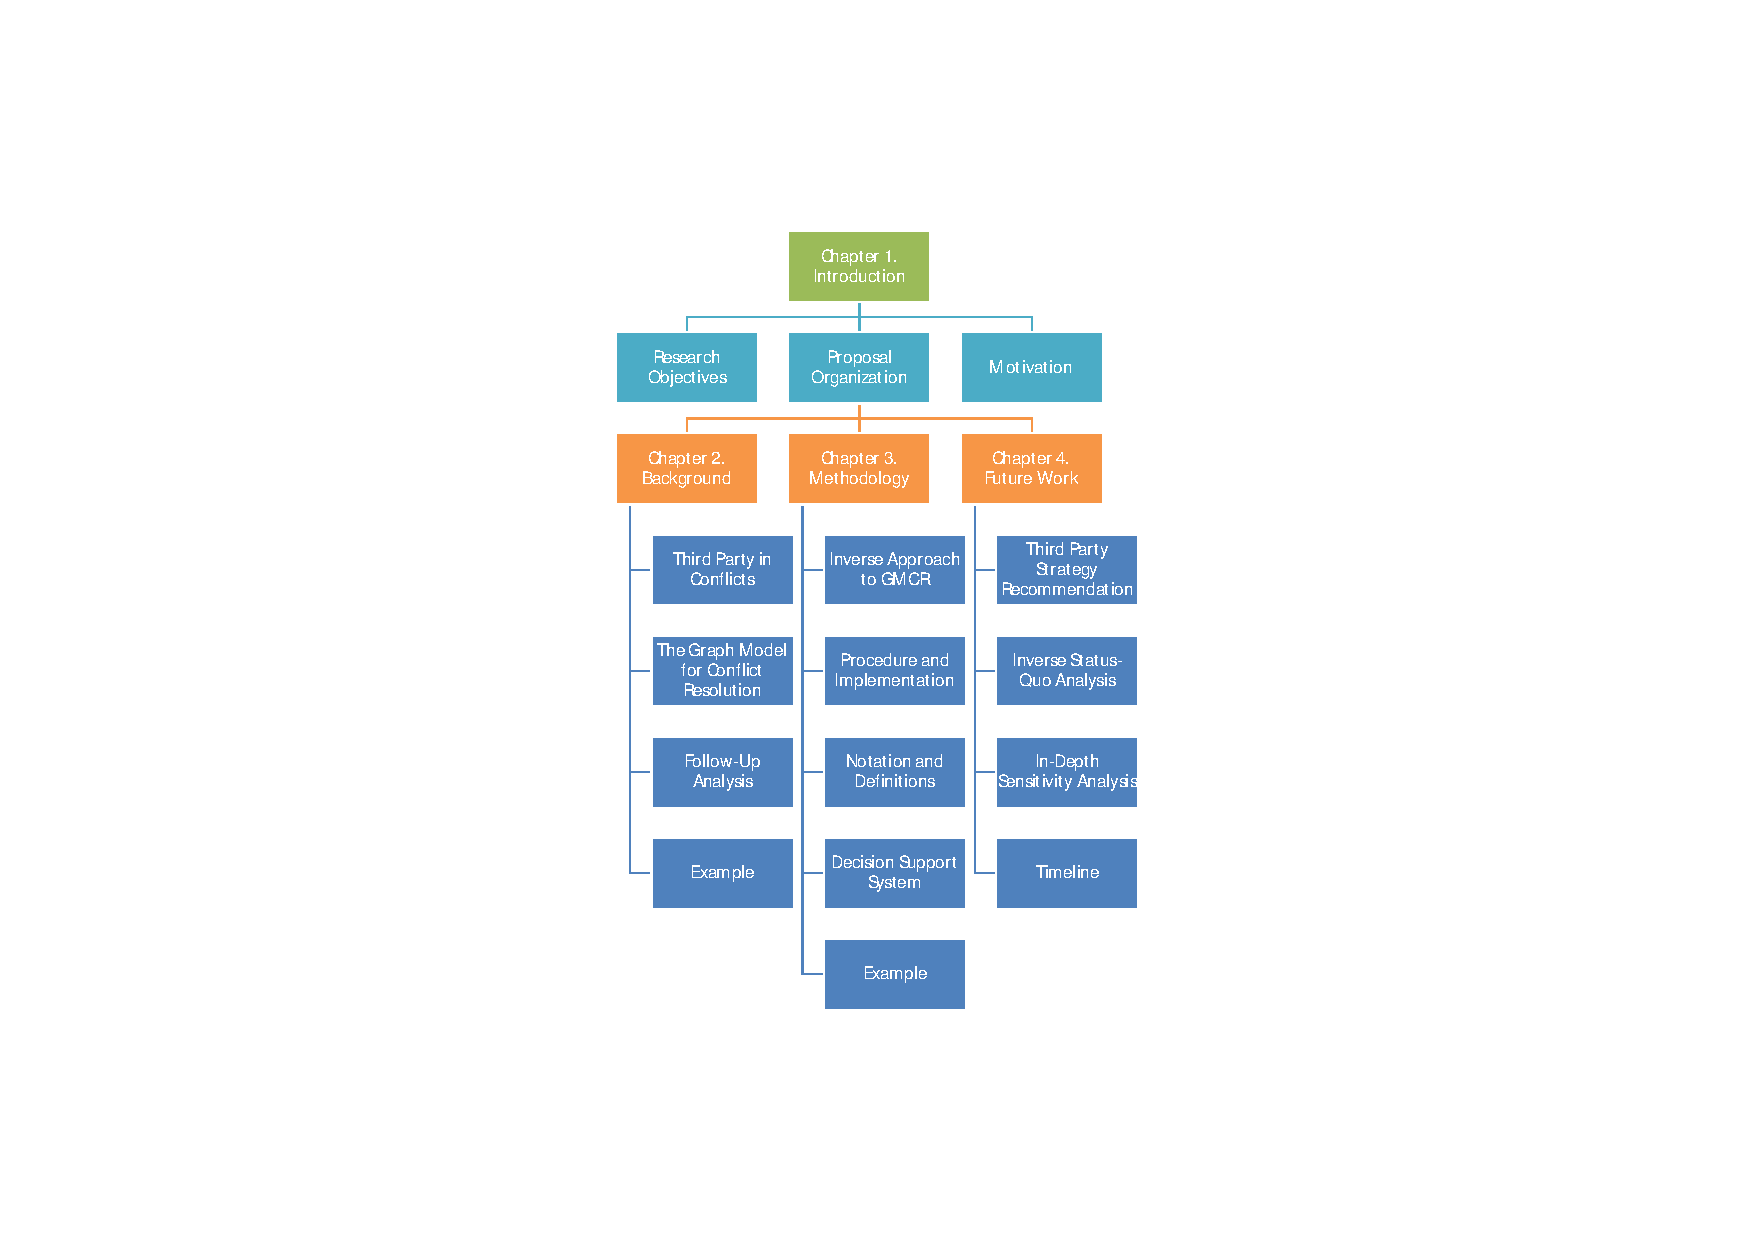
\includegraphics[scale=1]{PDF-IMG/proposalorganization.pdf}

\caption{Proposal Organization}

\label{fig:proposal}
\end{figure}
\end{center}


%======================================================================

% % % Literature % % %


\chapter{Background}


%%%%%%%%%%%%%%%%%%%%%%%%%%%%%%%%%%%%%%%%%%
%%%%%%%%%%%%%%%%%%%%%%%%%%%%%%%%%%%%%%%%%%


\section{Third Party in Conflicts}

Research into the impact of a third party in conflict resolution is reviewed in this section. The first subsection discusses the different types of conflict and the impact of third party intervention on them. Subsections \ref{sec:tproles} and \ref{sec:miscissues} discuss the possible roles of a third party, in addition to other issues. Finally, subsection \ref{sec:tpmodel} reviews the existing modeling approaches for third party intervention.

\subsection{Overview and Conflict Types}
\label{sec:ovrct}
Third party intervention in conflicts has been widely investigated from different perspectives. Most of the research lies within the areas of international relations and political sciences. These studies address  issues regarding mediation including methods of intervention \citep{fisher2001}, strategies for intervention \citep{prein1987}, and conditions for successful intervention \citep{regan1996}. 
Conflicts can be classified in a wide variety of ways. In the world of mediation, the differentiation between intrastate and interstate conflicts is usually clear. A study by \citet{regan1996} focuses on success conditions for third party interventions in intrastate conflicts. Another classification by \citet{bercovitch2006} differentiates between high intensity conflicts and low intensity conflicts. Another categorization for conflicts is based on cause, including ethnic, religious, or ideological \citep{regan1996}.  The size of the conflict, or the number of parties involved provides one more means for classification \citep{jehn1997}

\subsection{Third Party Roles}
\label{sec:tproles}
A third party can assume different roles in a conflict. \citet{sakamoto2005} suggested three roles a third party can undertake in a conflict. These roles are commonly assumed when the mediator is not an actual party in the conflict, but is motivated to bring about a more preferred resolution. The suggested three roles are arbitrator, coordinator, and donor. The authors explain each role within a conflict. A third party is an arbitrator if it has the power to restrict or force a stakeholder to accept a certain resolution. If a third party can alter stakeholders' preferences, then it is either a coordinator or a donor. The difference between the last two roles depends on the time of influence of the third party. A coordinator influences the stakeholder to change preferences immediately, while a donor works on the long term \citep{sakamoto2005}. On the other hand, \citet{raiffa1982} classifies third parties as facilitators, mediators, arbitrators, or rule manipulators. Another study suggests mediators can be individuals, regional organizations, states, or international institutions \citep{bercovitch2000,bercovitch2006}. The latter study surveyed 2,354 international conflicts involving mediation since 1945 in order to analyze them and assess various general hypotheses. Table \ref{tbl:tmad} summarizes their dataset. Some of their hypotheses will be outlined in subsection 2.1.4 of this proposal. 

\begin{center}
\begin{table}[h!]
\centering
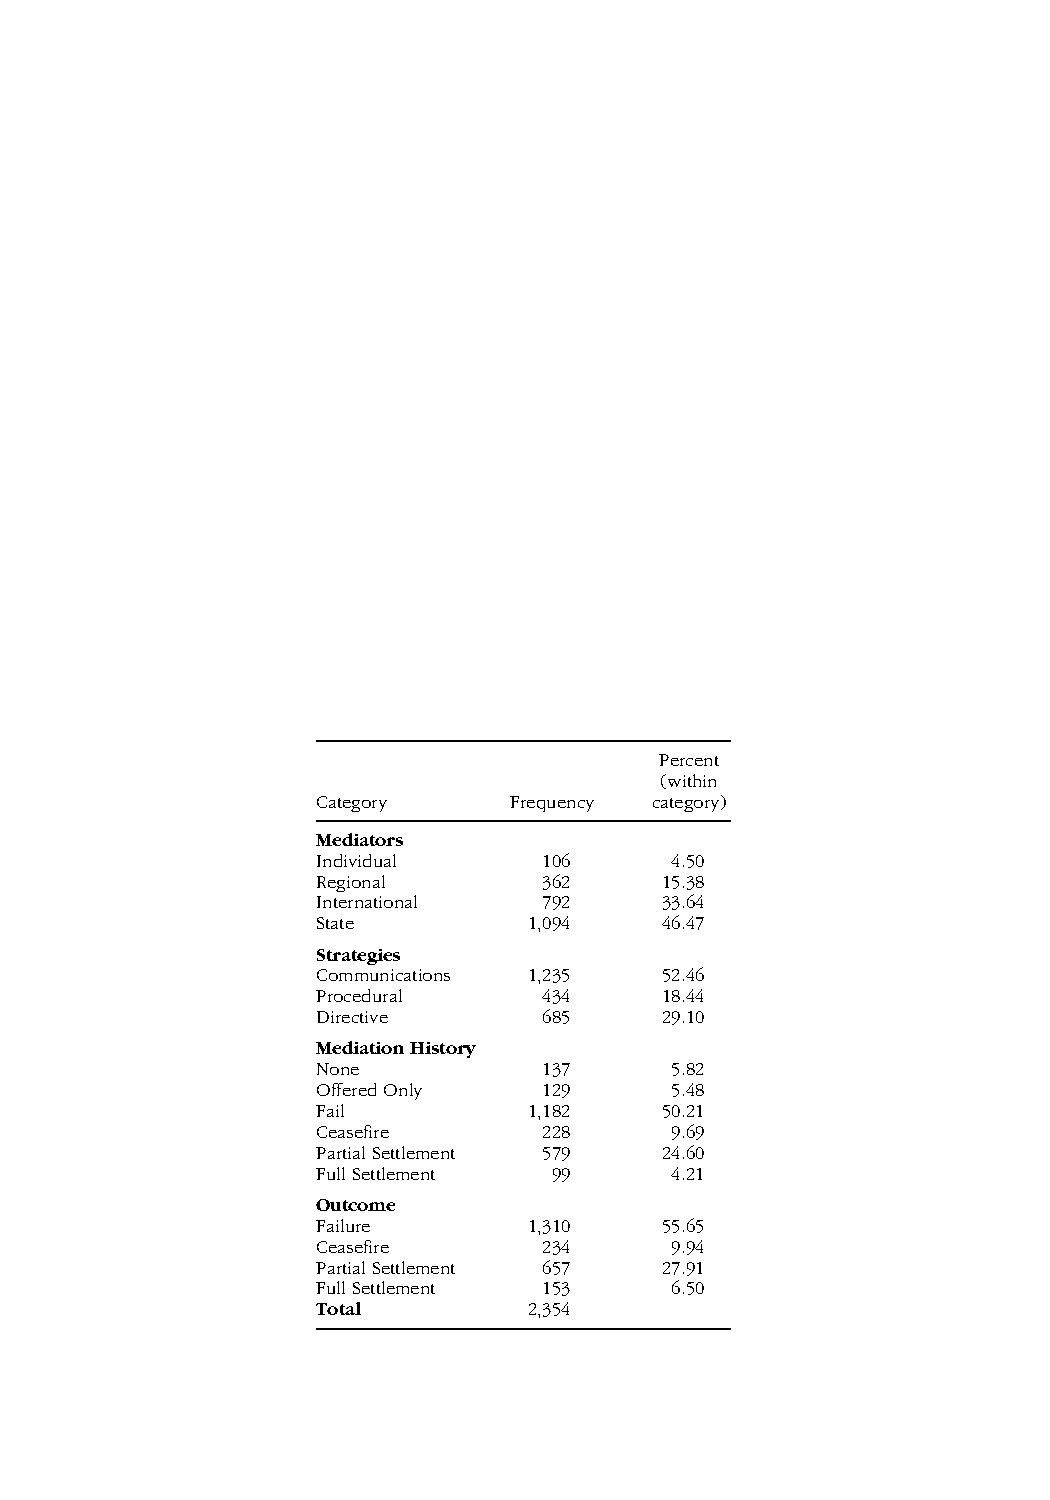
\includegraphics[scale=1]{PDF-IMG/table_mad.pdf}

\caption{Dataset Summary (Adopted from \citet{bercovitch2006}}

\label{tbl:tmad}
\end{table}
\end{center}

\subsection{Miscellaneous issues}
\label{sec:miscissues}
The literature is full of issues and factors affecting third party intervention. For example, factors affecting the process of intervention is that a mediator can act formally or informally, be invited to the conflict or not, intervene independently or on behalf of an organization, have interest in the outcome or in the process of intervention, be inclined toward one party or the other, and be consultative or directive in the intervention \citep{lewicki1992}. Furthermore, mediation history can also have an effect on a new intervention attempt \citep{bercovitch2006}. A study by \citet{carnevale2005} addresses the element of time. They found that time pressure affects the mediator to be aggressive in intervening and to use pressuring tactics. Other studies on the effectiveness of third party intervention suggest factors that influence the success of specific situations. For instance, if an uninvited third party intervenes, \citet{murray1983} specifies three important factors for mediation efficiency: dispute maturity, disputants' relationship, and intervention timing. Other issues raised by different researchers include culture, power asymmetries, conflict ripeness, number of third parties, third party authority, bias, and consistency \citep{fisher2001}.

Another aspect of mediation is strategy. The range of strategies a mediator can undertake is immense. \citet{regan1996} suggests three basic strategies of intervention within intrastate conflicts: military, economic, or mixed. \citet{young1972} discusses four intermediary functions: informational, tactical, supervisory, and re-conceptualization. In another study on successful mediation, \citet{bercovitch1991} outline different strategies that can be adopted by a third party: conciliation-facilitation, procedural, directive, substantive, and supervisory. The authors explain each of these strategies and assess their impact based on a range of historical conflicts. While these studies emphasize specific strategies, other approaches provide a more generic context, referred to as intervention styles. For instance, \citet{bartunek1975} organize intervention techniques into two broad styles: content form and process form. Another wide classification is that of Touval and Zartman, who categorize all intervention approaches as communication, formulation, or manipulation strategies \citep{bercovitch1993}.  \citet{bercovitch2006} suggest that all strategies can be grouped into communication, procedural, or directive strategies.

\subsection{Third Party Modeling}
\label{sec:tpmodel}
Many studies in the literature tackle third party intervention in the context of a specific historical conflict or set of conflicts such as the work by \citet{regan1996,bercovitch1991,dixon1996}.  For instance, the research by \citet{regan1996} on success conditions for third party interventions focuses only on intrastate conflicts and analyzes the conflicts occurred during the period between 1944 to 1994 (Table \ref{tbl:reganset}). The author suggests a regression model based on the dataset he gathered as illustrated in Fig \ref{fig:regansnap}.  The author emphasizes three intrastate conflict types: ethnic, religious, and ideological. Moreover, the regression model took into account other factors affecting the intervention such as the type of conflict, number of causalities, intervention type, and intervention target.
Other attempts to formally model third party intervention based on particular conflicts include the research by \citet{carment1996,HipelRami}. Although most third party modeling based on historical conflicts use regression analysis \citep{regan1996,dixon1996}, the latter two studies use game theory based models. In addition, \citet{fisher2001,lewicki1992} discuss different conceptual and descriptive models for third party intervention. Lastly, a standard conflict model of third party intervention is suggested by \citet{siqueira2003}.


\begin{center}
\begin{figure}[H]
\centering
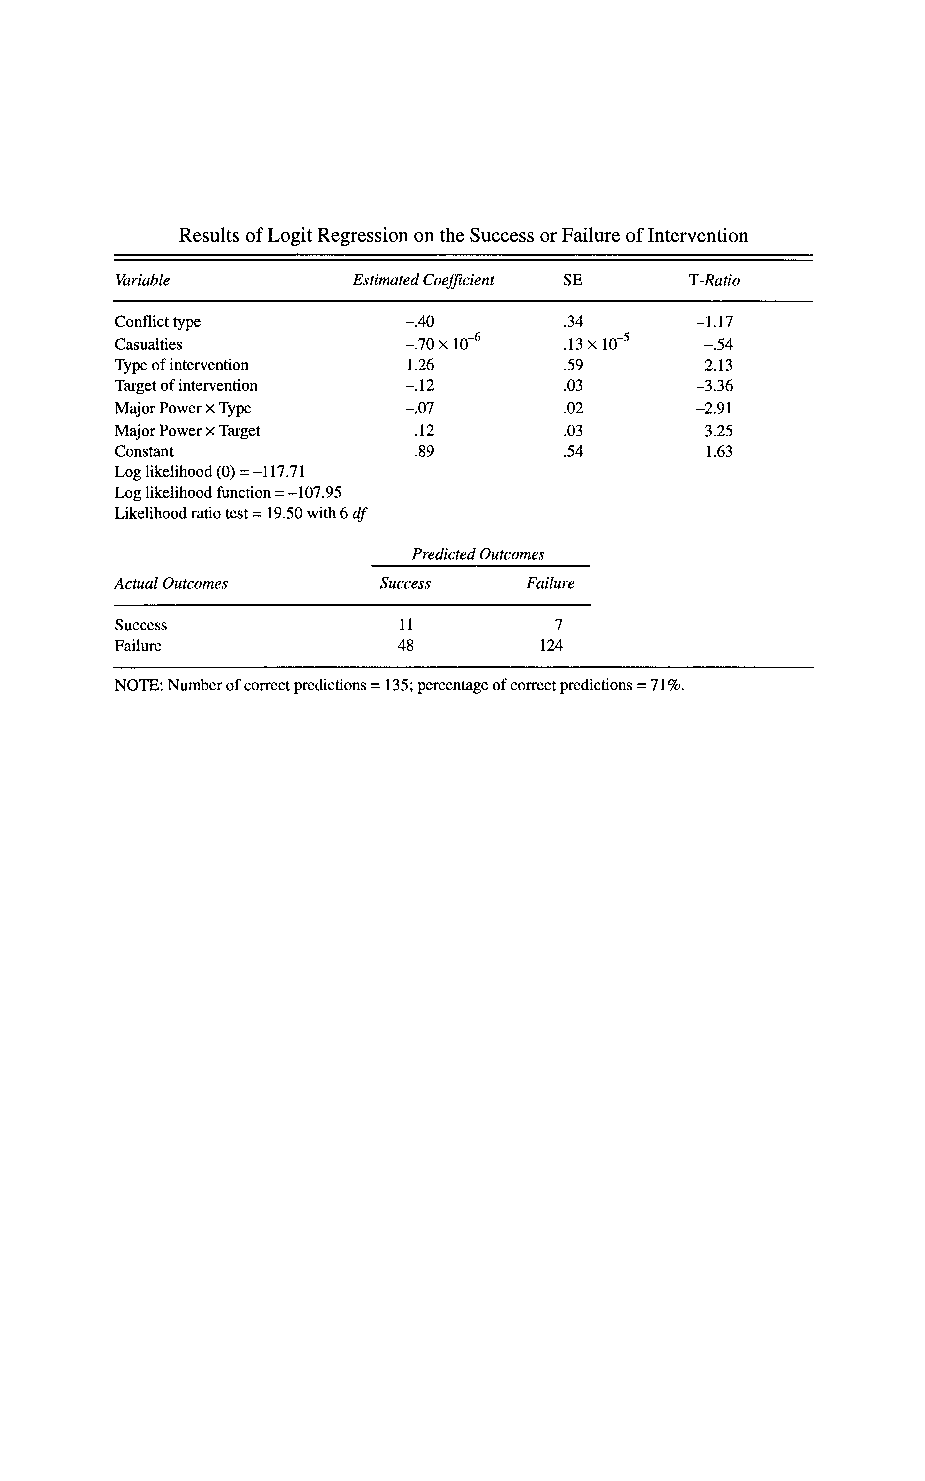
\includegraphics[scale=1]{PDF-IMG/Regan_snap.pdf}

\caption{A snapshot of the regression model by \citet{regan1996} with the results applied to the study dataset}

\label{fig:regansnap}
\end{figure}
\end{center}

\begin{center}

\begin{table}[H]
\centering
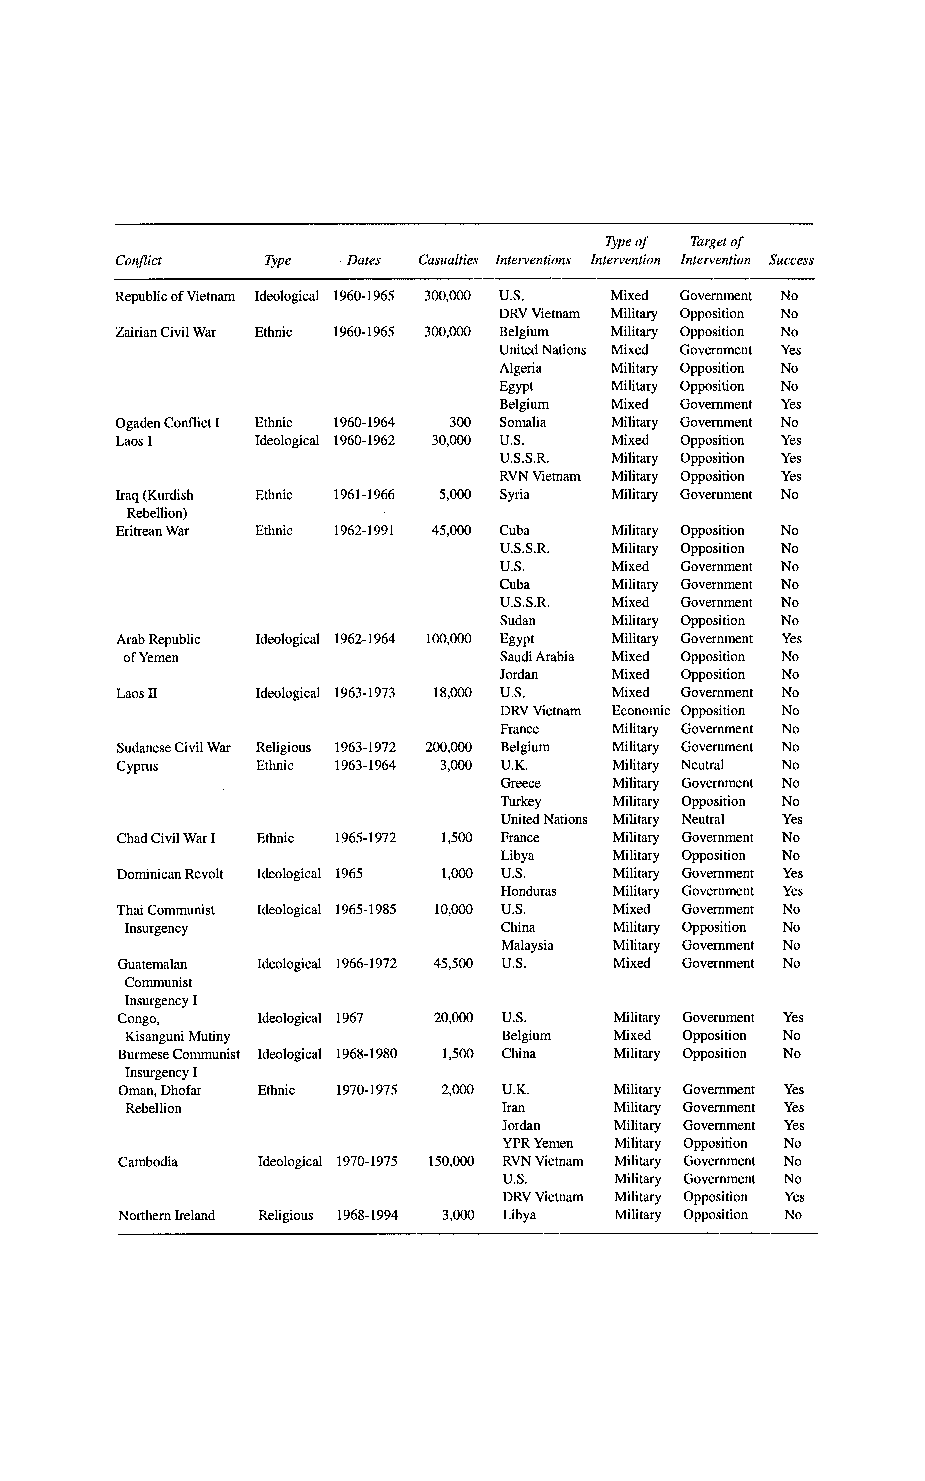
\includegraphics[scale=1]{PDF-IMG/Regan_set.pdf}

\caption{A dataset segment of the Intrastate Conflicts used in Regan's study (Table adopted from \citet{regan1996}}

\label{tbl:reganset}
\end{table}

\end{center}


A study by \citet{sakamoto2005} illustrates an approach to incorporate third party intervention in conflict modeling using GMCR. The research suggests three roles a third party can play (explained in subsection 2.1.2 of this report) and developed a conflict management procedure for them. Fig \ref{fig:sakamato_flow} below illustrates the authors' conflict management approach with the intervention of a third party.

\begin{center}
\begin{figure}[H]
\centering
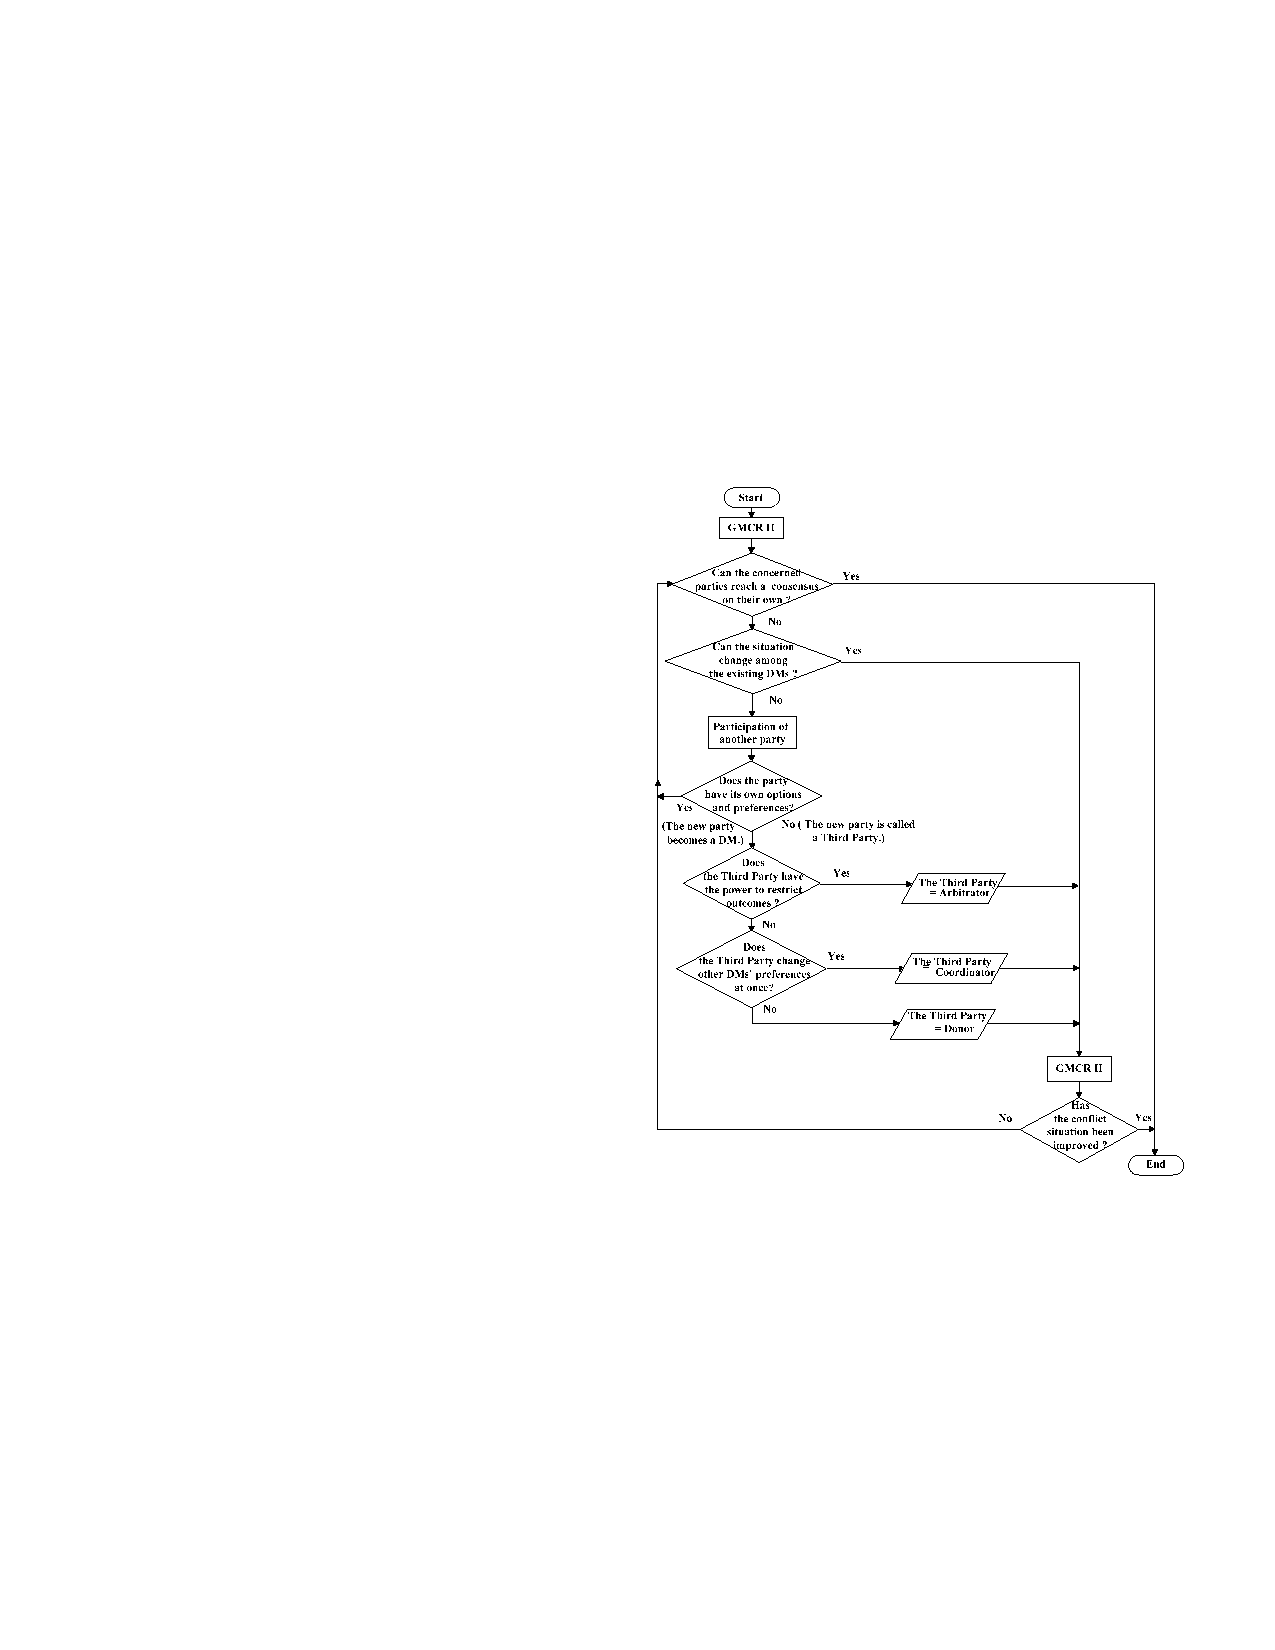
\includegraphics[scale=1]{PDF-IMG/sakamato_flow.pdf}

\caption{Chart developed by \citet{sakamoto2005} to illustrate conflict management with a third party}

\label{fig:sakamato_flow}
\end{figure}
\end{center}

A comprehensive study by \citet{bercovitch2006} investigates in depth the success factors of third party intervention. The authors focus on mediators' identities, strategies, and mediation history to predict the outcome of mediation. According to the authors, mediators can be classified according to four categories: individuals, states, regional organizations, and international institutions. After discussing each category, the authors claim that in low intensity conflicts, state and regional mediators are more likely to be successful. However, they are less likely to be successful in high intensity conflicts. International mediators are likely to be effective in high intensity conflicts and individuals are unlikely to be successful in all conflict types.
On the other hand, the authors suggest that mediation strategies include communication-facilitation, procedural, and directive strategies. Similarly, the authors make some hypotheses after explaining each of the strategies. They claim that directive strategies are most likely to be successful in high intensity conflicts but not in low intensity conflicts. Procedural strategies are mostly successful in low intensity conflicts. Tables \ref{tbl:MEDIATOR_TYPE} and \ref{tbl:MEDIATOR_STR} are summaries derived from the research hypotheses in the study. 

\begin{center}

\begin{table}[H]
\centering
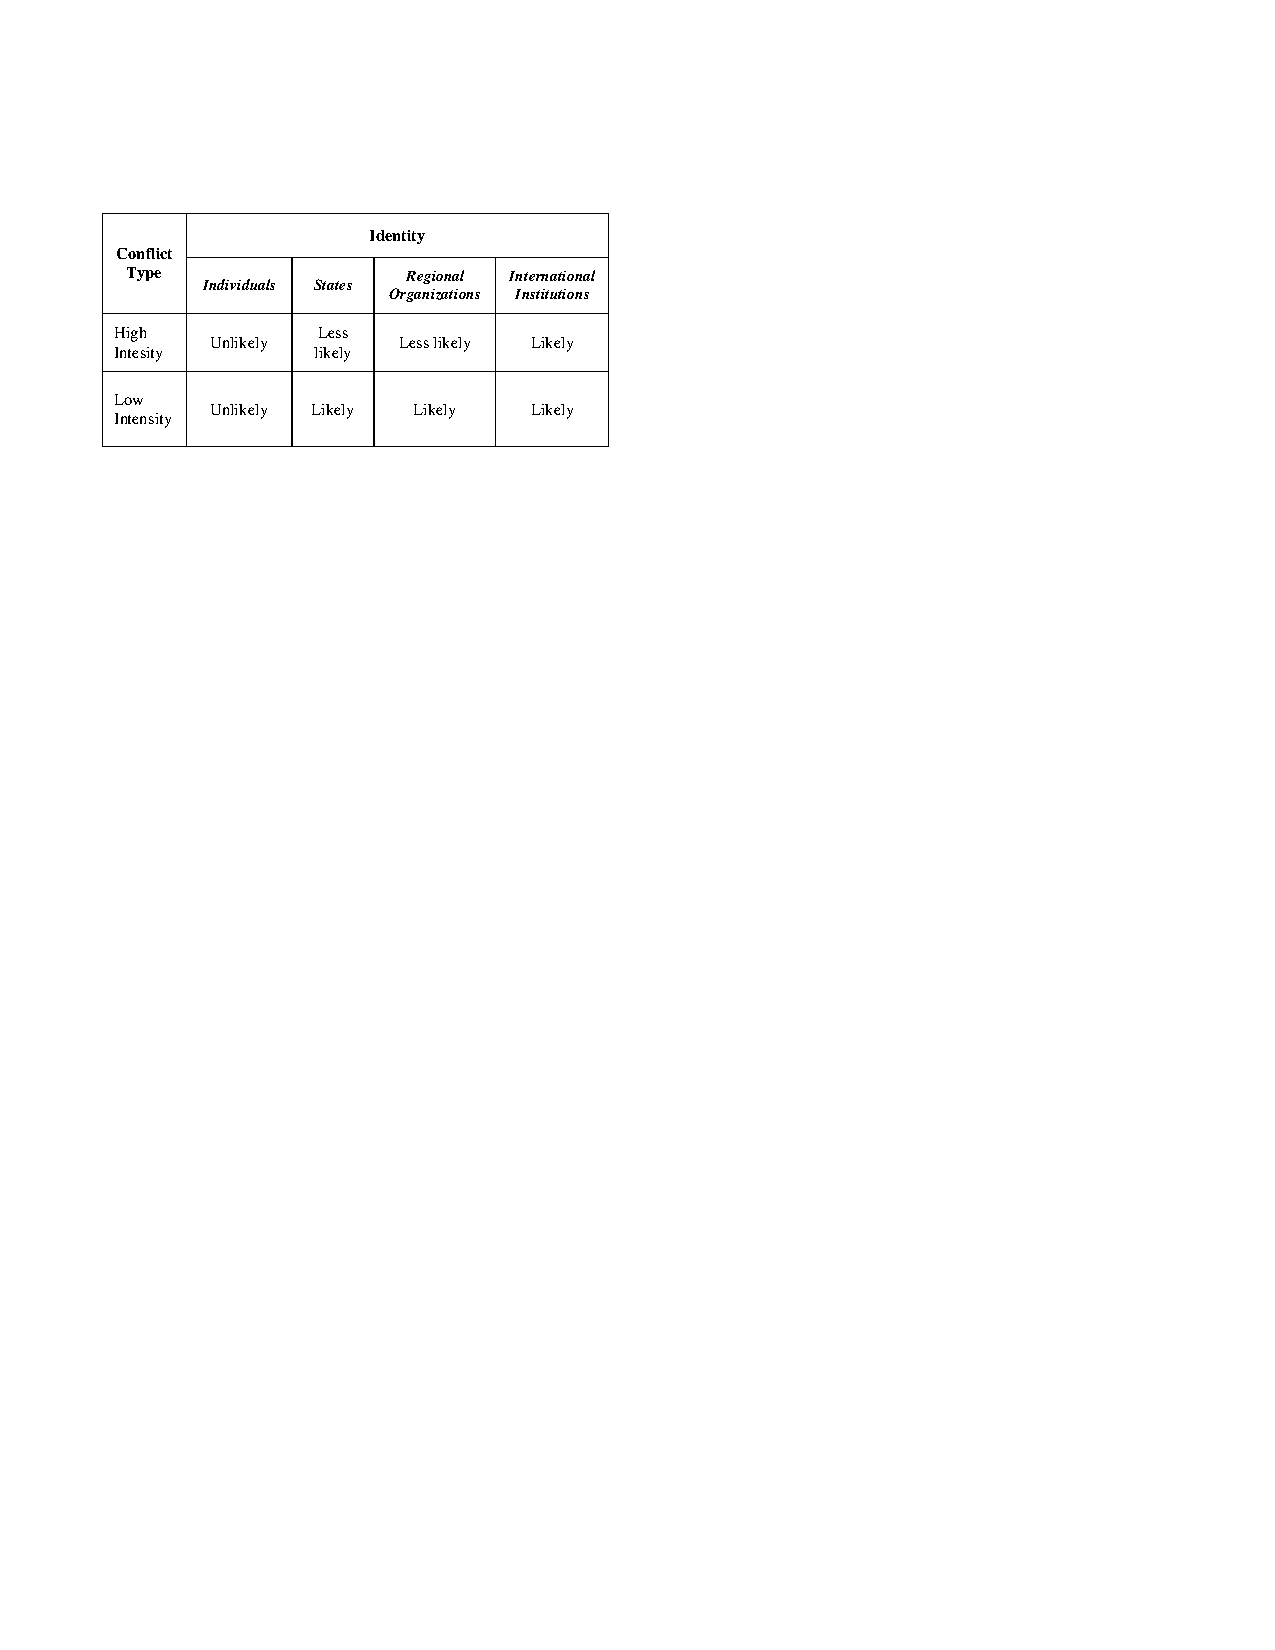
\includegraphics[scale=1]{PDF-IMG/MEDIATOR_TYPE.pdf}

\caption{Mediator type and likelihood to be successful}

\label{tbl:MEDIATOR_TYPE}
\end{table}

\end{center}

\begin{center}

\begin{table}[H]
\centering
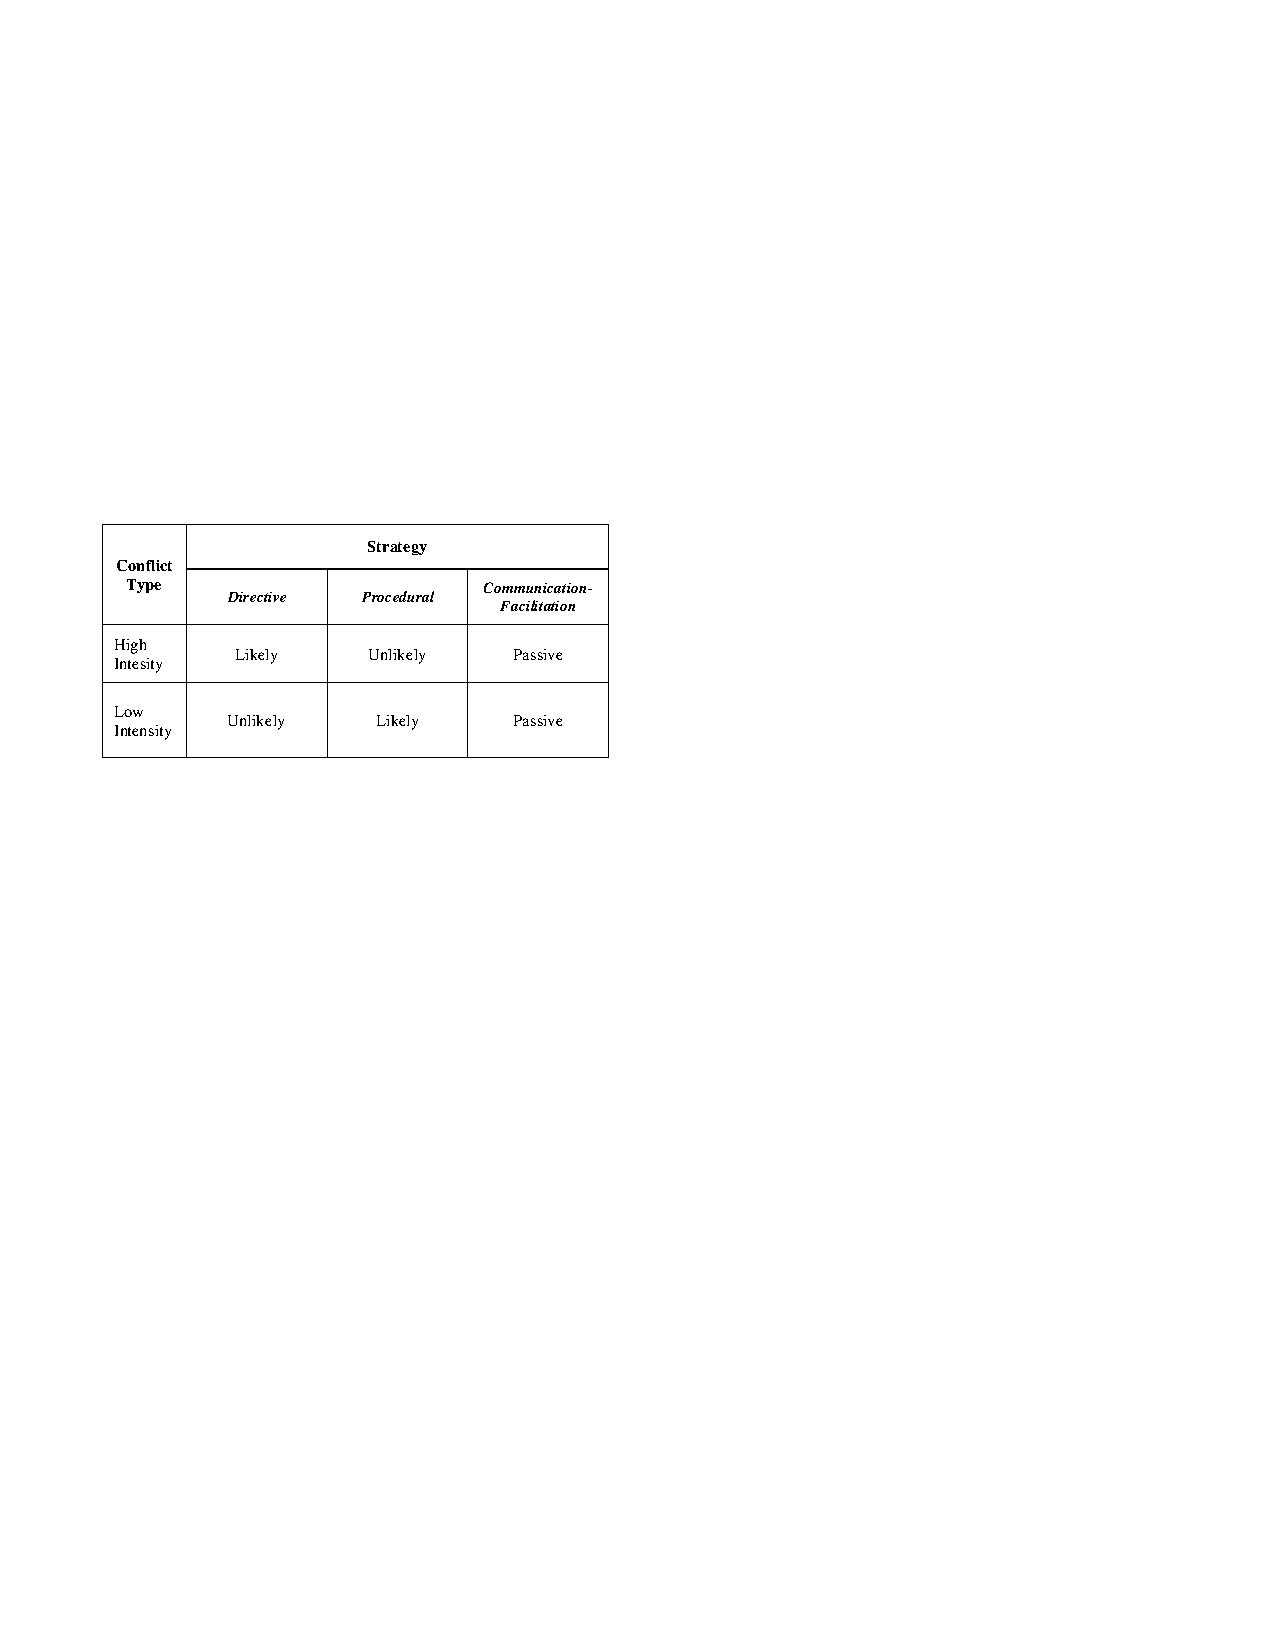
\includegraphics[scale=1]{PDF-IMG/MEDIATOR_STR.pdf}

\caption{Mediator strategy and likelihood to be successful}

\label{tbl:MEDIATOR_STR}
\end{table}
\end{center}

%%%%%%%%%%%%%%%%%%%%%

\section{The Graph Model for Conflict Resolution (GMCR)}
The Graph Model for Conflict Resolution (GMCR) has been developed and expanded since the mid-1980s \citep{kilgour2005}. GMCR is a tool to strategically analyze moves and counter moves in a conflict in order to predict the most likely outcome. 
\subsection{Procedure}
The basic procedure of GMCR involves two main stages: modeling and analysis. In the modeling stage, the user identifies the conflict parameters which include:
\begin{itemize}
\item Decision makers (DMs)
\item Options for each DM
\item Infeasible states (such as mutually exclusive situations)
\item Allowable transitions
\item Relative preferences
\end{itemize}

After identifying the conflict parameters, the user will analyze the conflict from each DM's perspective to determine the likely final resolution. This stage include:
\begin{itemize}
\item Determining individual stability (i.e. for each DM)
\item Overall equilibria
\item Sensitivity analysis
\end{itemize}

The following diagram in Figure \ref{fig:procedure_or} illustrates the basic GMCR procedure (The diagram is adapted from \citet{fang1993}).

\begin{center}
\begin{figure}[h!]
\centering
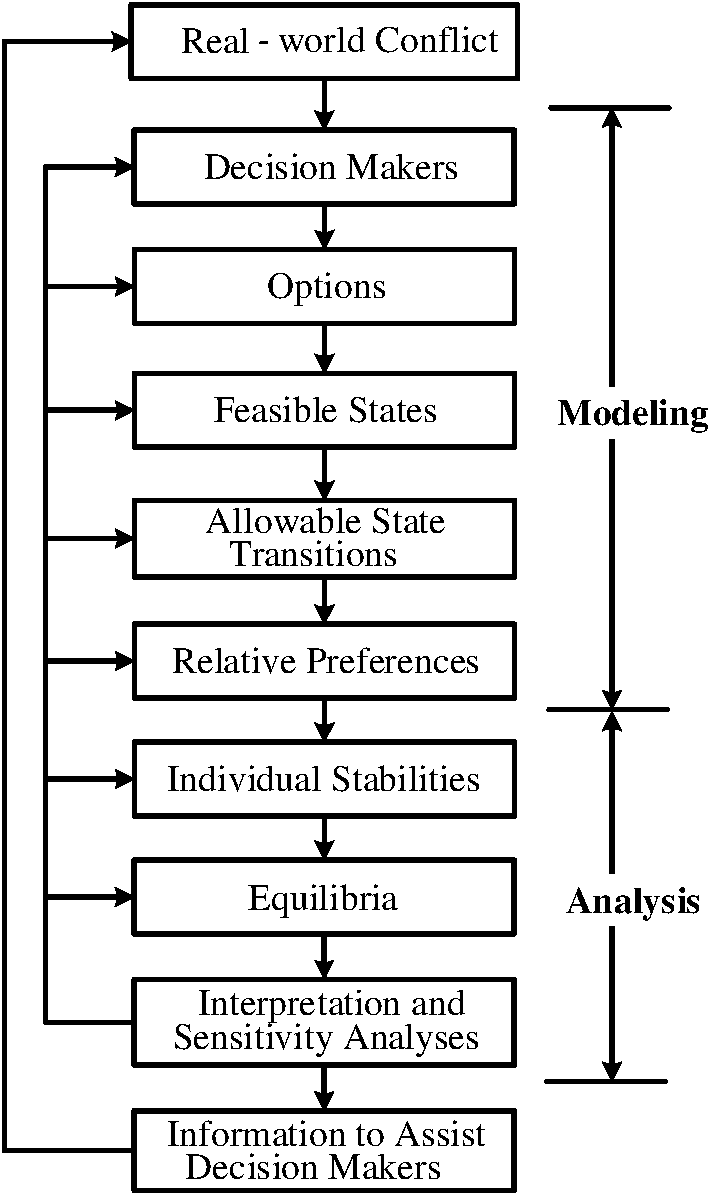
\includegraphics[scale=0.65]{PDF-IMG/GMCR_pro.pdf}

\caption{The basic procedure of GMCR in a real world conflict (adapted from \citet{fang1993})}

\label{fig:procedure_or}
\end{figure}
\end{center}

\subsection{Notation and Definitions}
The graph model representing a real world conflict includes DMs, options, and preferences. These parameters are formally defined as follows:

\begin{definition}
\rm
Let $N=\{1,2,\dots,n\}$ represent the set of DMs, for each DM $i \in N$, the set $O_{i}$ is $i$'s options or strategy set and $S=\{s_1, s_2, ..., s_m\}$ represent the set of feasible states.
\end{definition}

The set of possible states in a conflict is represented by the expression $2^o$ where $o$ is the total number of options in a conflict. Some of the possible states may be infeasible such as mutually exclusive options, at least one type of options, or dependent options. In a conflict model, a set of feasible states is defined.
%Cartesian product $S_{1} \times S_{2} \times \dots \times S_{n}$

\begin{definition}
\rm
Let  $S=\{s_1, s_2, ..., s_m\}$ represent the set of feasible states in a conflict. For each DM $i \in N$, a set of directed graphs $D_{i}=(S,A_{i})$ can be used to model the conflict.
\end{definition}


The feasible states of a conflict are represented by vertices in the graph model. In each graph, an arc $A_{i}$ exists between states $s_a$ and $s_b$ $\in$ $S$ if DM $i$ can move unilaterally in one step between the two states. It is called a \emph{directed} graph because the arc has an orientation which can be one way (irreversible move) or two ways (reversible move).

\begin{definition}
\rm
Let $i \in N$ and $s \in S$. The reachable list of DM $i$ from state $s \in S$ is defined as:
$$R_i(s)=\{s_a \in S \quad : \quad (s, s_a) \in A_i\}$$
\end{definition}

The move in one step by DM $i$ from a state $s_a$ to a state in the reachable list $\{s_b\in S\}$ is called a unilateral move (UM).

The preference information of DM $i$ is a binary relation $\{\succ_i,\sim_i\}$ over $S$, where $s_a\succ_i s_b$ means that DM $i$ prefers $s_a$ to $s_b$ and $s_a\sim_i s_b$ means that DM $i$ is indifferent between states $s_a$ and $s_b$. The binary relation $\{\succ_i,\sim_i\}$ is considered complete.

\begin{definition}
\rm
Let $i \in N$ and $s \in S$. The unilateral improvement list for DM $i$ from state $s \in S$ is defined as:
$$R_i^+(s)=\{s_a \in R_i(s) \quad : \quad s_a\succ_i s\}.$$
\end{definition}

The move in one step by DM $i$ from a state $s_a$ to a state in the unilateral improvement list $\{s_b\in S\}$ is called a unilateral improvement (UI).

\subsection{Stability Definitions and Solution Concepts}

The main goal of the graph model for conflict resolution is to predict the stability of each state for each DM. There are four basic solution concepts according to which a state can be assessed for stability: Nash stability (sometimes called rationality), sequential stability (SEQ), general metarationality (GMR), and  symmetric metarationality (SMR). 

The solution concepts describe how a DM is motivated to make moves and counter moves. These concepts (or behavior patterns) determine whether a specific state will be terminal or a DM will be motivated to deviate to another state. Different DMs may have different behavior patterns based on different factors. These factors include risk, foresight, and available information. Behavioral characteristics according to the different solution concepts are given in Table \ref{tbl:behchar} below. 

\begin{definition}
\rm {\bf (Nash Stability)} Let $i \in N$ and $s \in
S$. State $s$ is \emph{Nash stable} for DM $i$ \emph{iff} $R_i^+(s)=\phi$.
\end{definition}

\begin{definition}
\rm {\bf (Sequential Stability)} Let $i \in N$ and $s \in
S$. State $s \in S$ is \emph{sequentially stable} (\emph{SEQ}) for DM $i$ \emph{iff} for every $s_1 \in R_i^+(s)$ there exists at least one $s_2 \in R_{N-i}^+(s_1)$
such that $s_2 \precsim_i s$.
\end{definition}

\begin{definition}
\rm {\bf (General Metarationality)} Let $i \in N$ and $s \in
S$. State $s \in S$ is \emph{general metarational} (\emph{GMR}) for DM $i$ \emph{iff} for every $s_1 \in R_i^+(s)$ there exists an $s_2 \in
R_{N-i}(s_1)$ such that $s_2 \precsim_i s$.
\end{definition}

\begin{definition}
\rm {\bf (Symmetric Metarationality)}  Let $i \in N$ and $s \in
S$. State $s \in S$ is \emph{symmetric metarational} (\emph{SMR}) for DM $i$ \emph{iff} for every $s_1 \in R_i^+(s)$ there exists an $s_2 \in
R_{N-i}(s_1)$ such that $s_2 \precsim_i s$ and $s_3 \precsim_i s$
for all $s_3 \in R_k(s_2)$.
\end{definition}

\begin{table}[H]
\centering
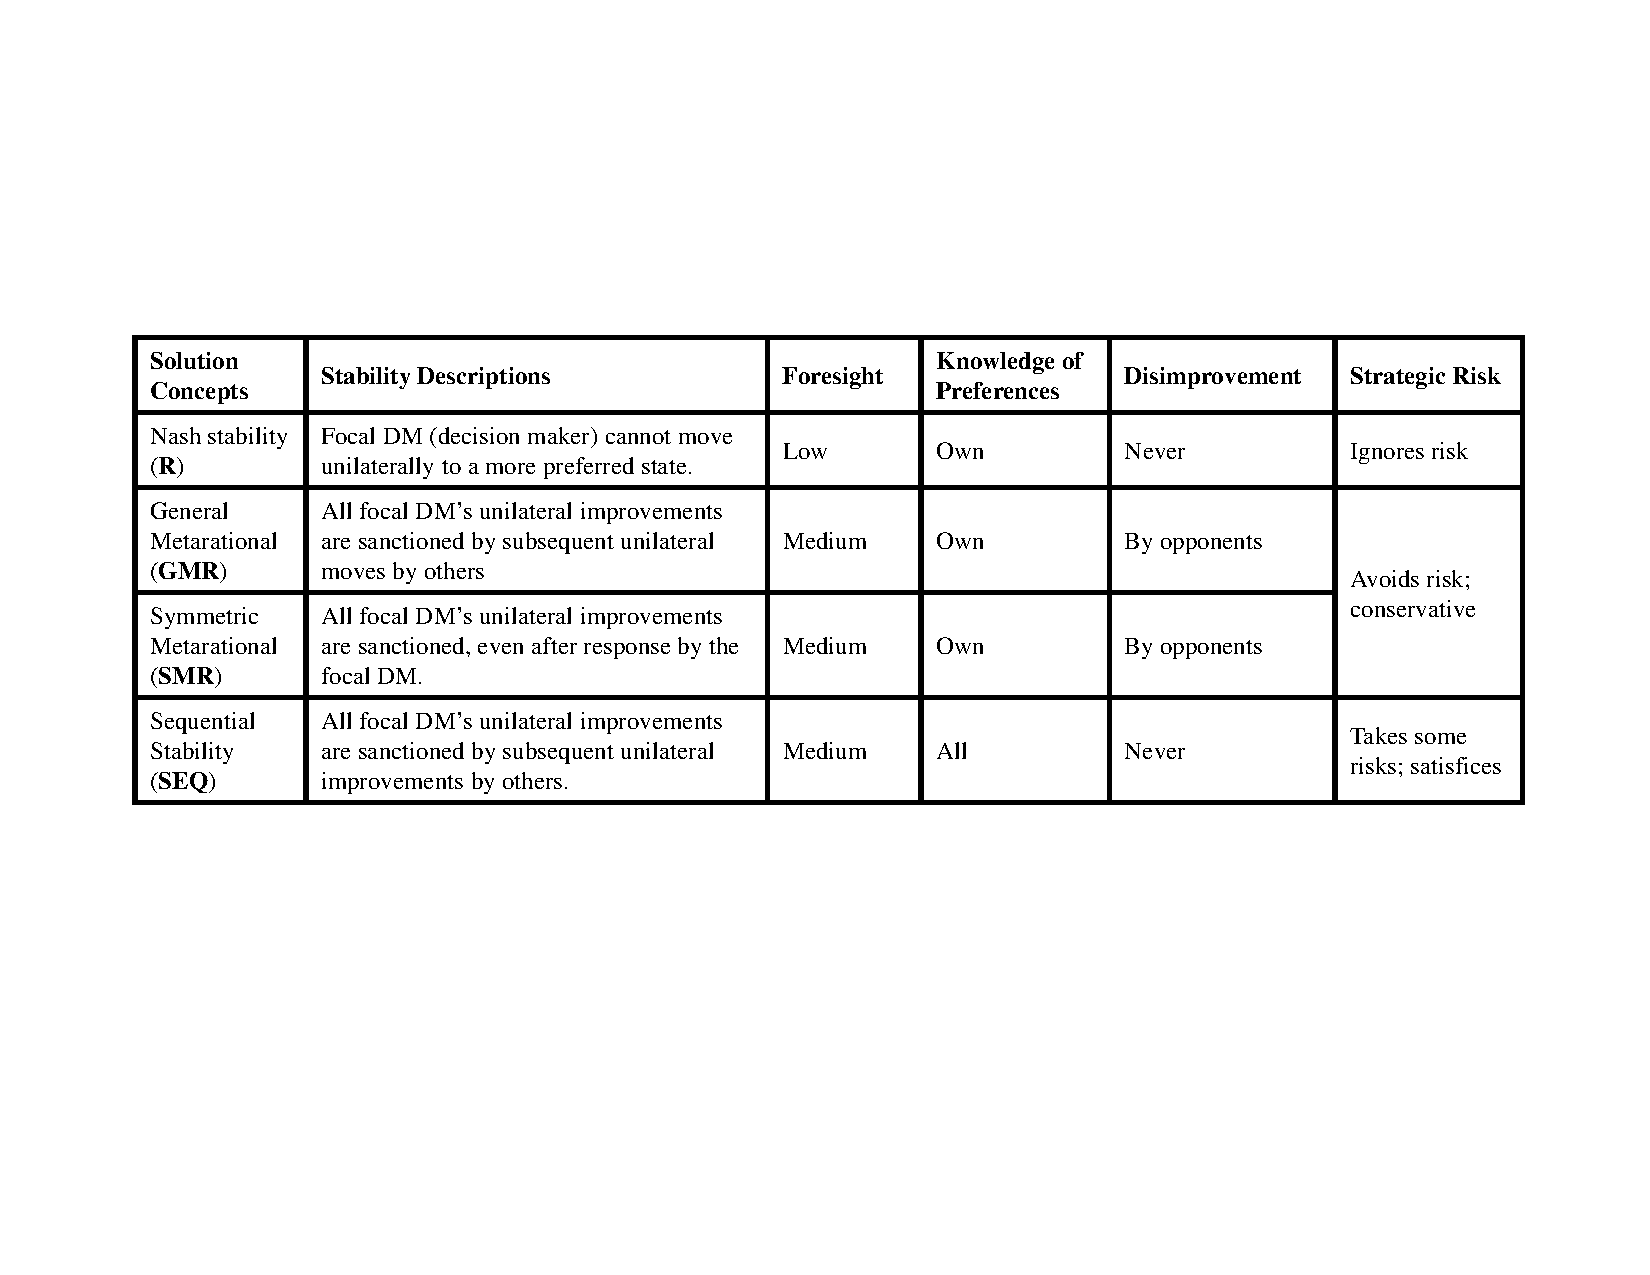
\includegraphics[scale=.75]{PDF-IMG/tablecomp.pdf}

\caption{Behavioral characteristics describing different solution concepts}

\label{tbl:behchar}
\end{table}

\begin{definition}
\rm {\bf (Equilibrium)}  Let $i \in N$ and $s \in
S$. State $s \in S$ is called \emph{equilibrium} (\emph{E}) \emph{iff} it is stable for every DM.
\end{definition}

Sometimes the graph model for conflict resolution is referred to as a 3-tuple or triplet $G=\langle N,S,(\succ_i,\sim_i)_{i\in N}\rangle$ where $N$ is the list of DMs $N=\{1,\dots ,n\}$, $S$ is the set of feasible states $S=\{1,\dots ,m\}$, and $(\succ_i,\sim_i)$ is the binary relation DM $i$ has on $S$. Consequently, $Nash(G)=\{ \enskip s \in S \enskip : \enskip s \enskip$  is a Nash Equilibrium of $G \}$. More explicitly, $$Nash(N,S,(\succ_i,\sim_i)_{i\in N})=\{ \enskip s \in S \enskip : \enskip s \enskip  \text{is Nash stable for all } i \in N \text{ in } \langle N,S,(\succ_i,\sim_i)_{i\in N}\rangle \}$$ and similarly for SEQ, GMR, and SMR.

%%%%%%%%%%%%%%%%%%%%%

\section{Follow-Up Analysis}

To take the basic analysis further, a number of follow-up analyses may be undertaken to test the reliability of the predicted outcomes and whether they are achievable from the status quo or not.

\subsection{Sensitivity Analysis}

Since many conflict parameters are subjective, it may be essential to test different scenarios in order to determine the robustness of the conflict model. Sensitivity analysis also points out how different parameters can influence the stability results. The most common type of sensitivity analysis is the change of preference since it is the most difficult parameter to obtain and determine. Other sensitivity analysis types include:

\begin{itemize}
\item Adding or combining DMs
\item Change of options (adding, removing, or modifying) 
\item Changing moves reversibility
\item Coalition analysis
\item Modeling misunderstandings (hypergames)
\item Examining other patterns of human behavior
\end{itemize}

%%%%%%%%%%%%%%%%%%%%%

\subsection{Status Quo analysis}

Every real world conflict has a starting point from which the conflict evolves. This point or state is called \emph{status quo} \citep{fang1993}. Depending on the status quo, a potential equilibrium may or may not be reached. \citet{li2004squo,li2005squo} developed algorithms and formal definitions to inspect the attainability of a potential resolution (\emph{equilibrium}) from a certain state (\emph{status quo}).
%%%%%%%%%%%%%%%%%%%%%

\section{Strategic Investigations of Water Conflicts in the Middle East using GMCR}
\label{sec:example1}
It was noted earlier in the introduction that a recent study on water conflicts emphasized the effect of third party intervention in bringing about a resolution. This study will be summarized in this section. An in-depth analysis and background can be found in \citet{HipelRami}.

\subsection{Background}
The arid nature of the Middle East environment causes continuously escalating conflicts among the countries of the region. Conflicts arise as water resources dwindle due to increased industrial and agricultural projects and population growth. The main renewable sources of freshwater in the region are rivers. Like all water resources, they are replenished by their hydrological cycle, with renewal rates varying from days to centuries. The rate of renewal for Middle Eastern rivers is decreasing due to population growth and the increasingly arid conditions of the region. At 2,700 km, the Euphrates is the longest and arguably most important river in the Middle East (Southwest Asia) \citep{kolars1991euphrates}.
The Euphrates originates in eastern Anatolia in Turkey and flows through Syria and finally Iraq, where it joins the Tigris River. Conflicts regarding the river became serious during the 1960s, when Turkey began building dams on the Euphrates to generate electricity and increase the availability of irrigation water in Southeast Turkey \citep{akanda2007tigris}. As a result of external mediation, war was narrowly avoided twice, in 1975 and 1998 \citep{akanda2007tigris}.

The original study investigated three interconnected conflicts along the Euphrates River occurring in 1975, 1990, and 1998. This example will only focus on the conflicts that took place in 1975 and 1998 as both of them involved mediation. 

\subsubsection{The conflict in 1975}
In 1966, Turkey started the construction of the Keban Dam, which is a hydroelectric dam on the Euphrates River (Fig \ref{fig:dams}). After the construction was finished in 1974, Turkey started the filling of the Keban Reservoir. During the flooding, Turkey maintained a 450 $m^3/s$ discharge of the Euphrates to the two downstream countries consisting of Syria and Iraq. This rate was agreed upon by both countries through the United States Agency for International Development (USAID), which was financing the project \citep{inan2000law}. However, Syria also started filling the lake behind its newly constructed Thawra Dam. Simultaneously, the area was hit by a significant drought \citep{kalpakian2004identity}. As a result, the flow of the Euphrates River entering Iraq was reduced to a trickle. Iraq accused Syria of this reduction and of endangering the lives of three million Iraqi farmers dependent on river irrigation water \citep{morris1997water}. Iraq complained that the flow had dropped from the normal 920 $m^3/sec$ to an unacceptable 197 $m^3/sec$ \citep{priscoli2009managing}. Iraq requested an intervention by the Arab League; however, Syria argued that it was receiving less water from Turkey as well and refused to cooperate. As the tension increased, Syria closed its airspace to all Iraqi aircraft, suspended Syrian flights to Baghdad, and transferred troops from the Israeli border to the Iraqi frontier by May 1975 \citep{morris1997water}. Iraq also sent its troops to the shared border and threatened to bomb Syria's dam. 

Before the conflict could escalate any further, Saudi Arabia and the Soviet Union intervened - only mediation on the part of Saudi Arabia was able to alleviate the situation \citep{priscoli2009managing}. On June 3, 1975, an agreement between Iraq and Syria, with the mediation of Saudi Arabia, averted the impending war. The agreement stipulated that Syria is to release extra amounts of water to Iraq \citep{akanda2007tigris}: specifically, 58\% of what Syria receives from the Euphrates is to be released to Iraq \citep{priscoli2009managing}. In addition to resolving the conflict, Saudi Arabia contributed to a basin fund that would finance irrigation reform and other methods to reduce unmet demands \citep{akanda2007tigris}.

\begin{center}
\begin{figure}[h]
\centering
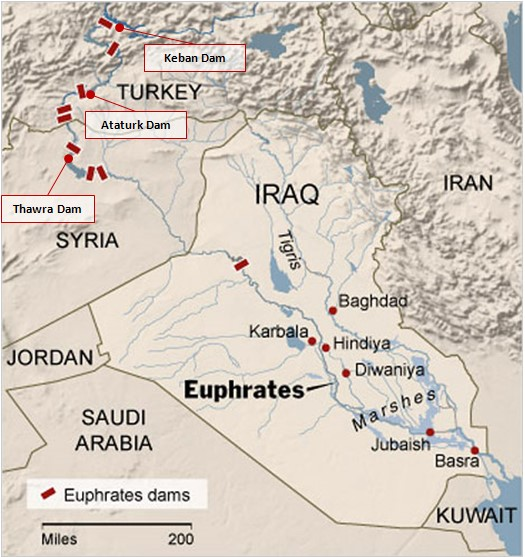
\includegraphics[scale=.6]{PDF-IMG/dams.jpg}

\caption{The Euphrates River along with the dams constructed on it (The New York Times, 2009)}

\label{fig:dams}
\end{figure}
\end{center}

\subsubsection{The Conflict in 1998}
Many events took place between the conflict in 1975 and prior to 1998. Mainly, an ironic coalition between Syria and Iraq against Turkey because of the latter's announcement of the largest water resources project in South-Eastern Anatolia known as the ``GAP Project", which includes 22 dams and 19 hydropower installations on the Euphrates-Tigris \citep{frenken2009irrigation}. In addition, tension increased between Turkey and Syria due to the latter support of the rebellion movement of the Kurdish Workers Party (PKK), which is struggling to create a Kurdish state in South Eastern Turkey \citep{guner1998signalling}. Syria's continuous support for the PKK was affecting Turkey's stability and depleting its resources. Despite bilateral security agreements between Syria and Turkey in 1992 and 1993, Turkey continued to accuse Syria of supporting the PKK, while Syria insisted that it forced the PKK to move its bases from Syrian territory in conformity with the bilateral agreements between itself and Turkey \citep{guner1998signalling}. In 1993, the Turkish Prime Minister declared that if Syria did not ban PKK from its country, there could be no solution to the water problem. The issue was raised again in the trilateral summit of 1994 between the Foreign Ministers of Turkey, Syria, and Iraq with no improvements. Moreover, in 1995, Turkey organized military operations in northern Iraq against PKK members who fled to Syria, thus confirming Turkish suspicions. Finally, in 1998, Turkey charged Syria with support of the PKK and harboring its leader, perhaps providing refuge to the leader in Damascus. Turkey escalated the situation and threatened to invade Syria. Egypt intervened and the Egyptian President, Hosni Mubarak, secured Syria's pledge to stop supporting the PKK \citep{akanda2007tigris}. On account of the intervention of Egypt and in order to avert an invasion by Turkey, the Syrian government agreed to ban PKK from Syria by signing the Adana Agreement on October 20, 1998 \citep{priscoli2009managing}. Finally, Table \ref{tbl:historyEuphrates} outlines the historical evolution of the most notable events related to the Euphrates conflicts.

\begin{table}[H]
\centering
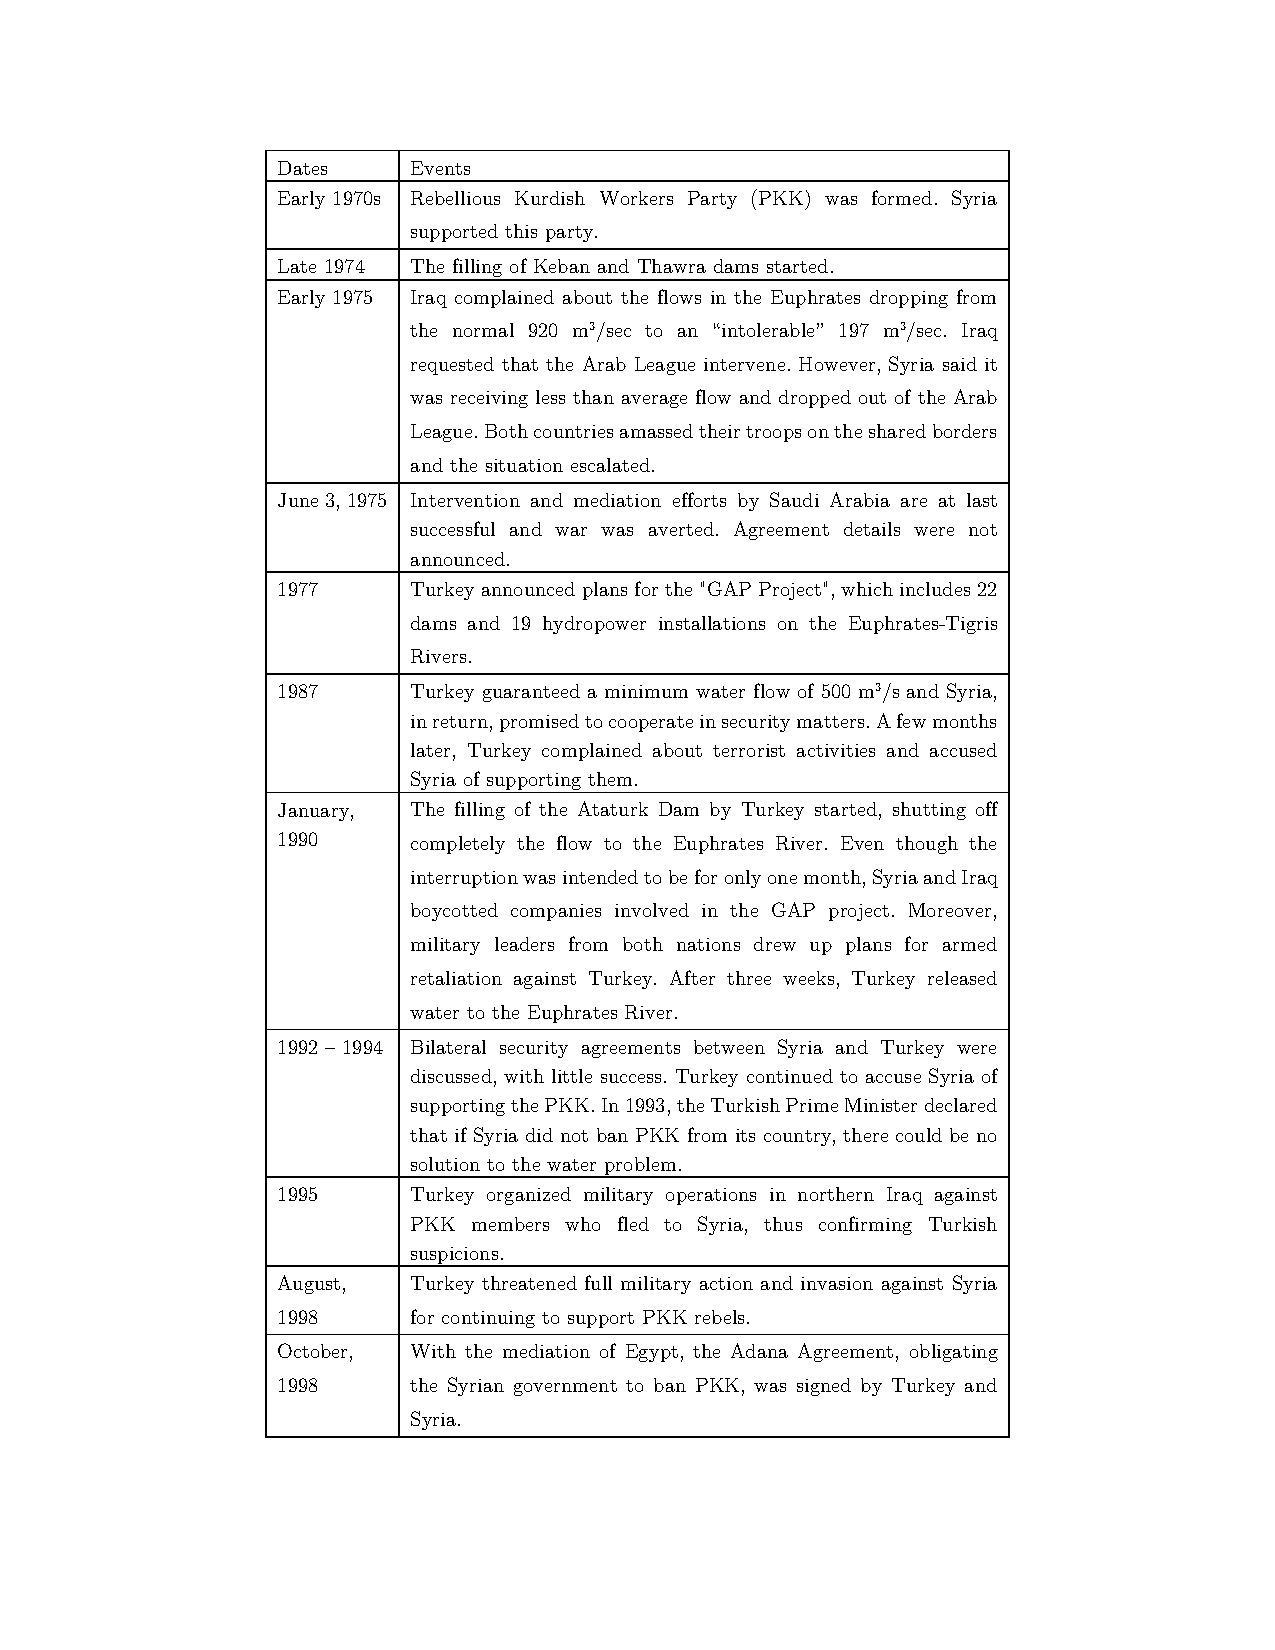
\includegraphics[scale=.88]{PDF-IMG/Euphrates_history.pdf}

\caption{Notable events related to conflicts along the Euphrates River}

\label{tbl:historyEuphrates}
\end{table}

%%%%%%%%%%%%%%%%%%%%%

\subsection{Conflict Analysis of the 1975 Dispute}
The DMs and options for the 1975 conflict are given in Table \ref{tbl:t1}. Notice that Syria has an option regarding the release of the water plus an option of escalating the situation. Iraq has the single option of attacking Syria. Since both Saudi Arabia and the Soviet Union have similar preferences and reasons for getting involved, they are considered as a single DM labeled as ``Third Party". The Third Party has a single option of acting or not. Table \ref{tbl:t1} describes the options for each DM. Each option is labeled with a number and can be either taken (Y for yes) or not (N for no). For example, option 3, which is entitled Attack, is the situation in which Iraq can use military action to force Syria to release water into the Euphrates. Undertaking this option, as indicated by Y for yes, means using force, while not taking this option, N for no, indicates accepting the situation and allowing Syria to fill the Thawra Dam without escalation.

\begin{table}[H]
\centering
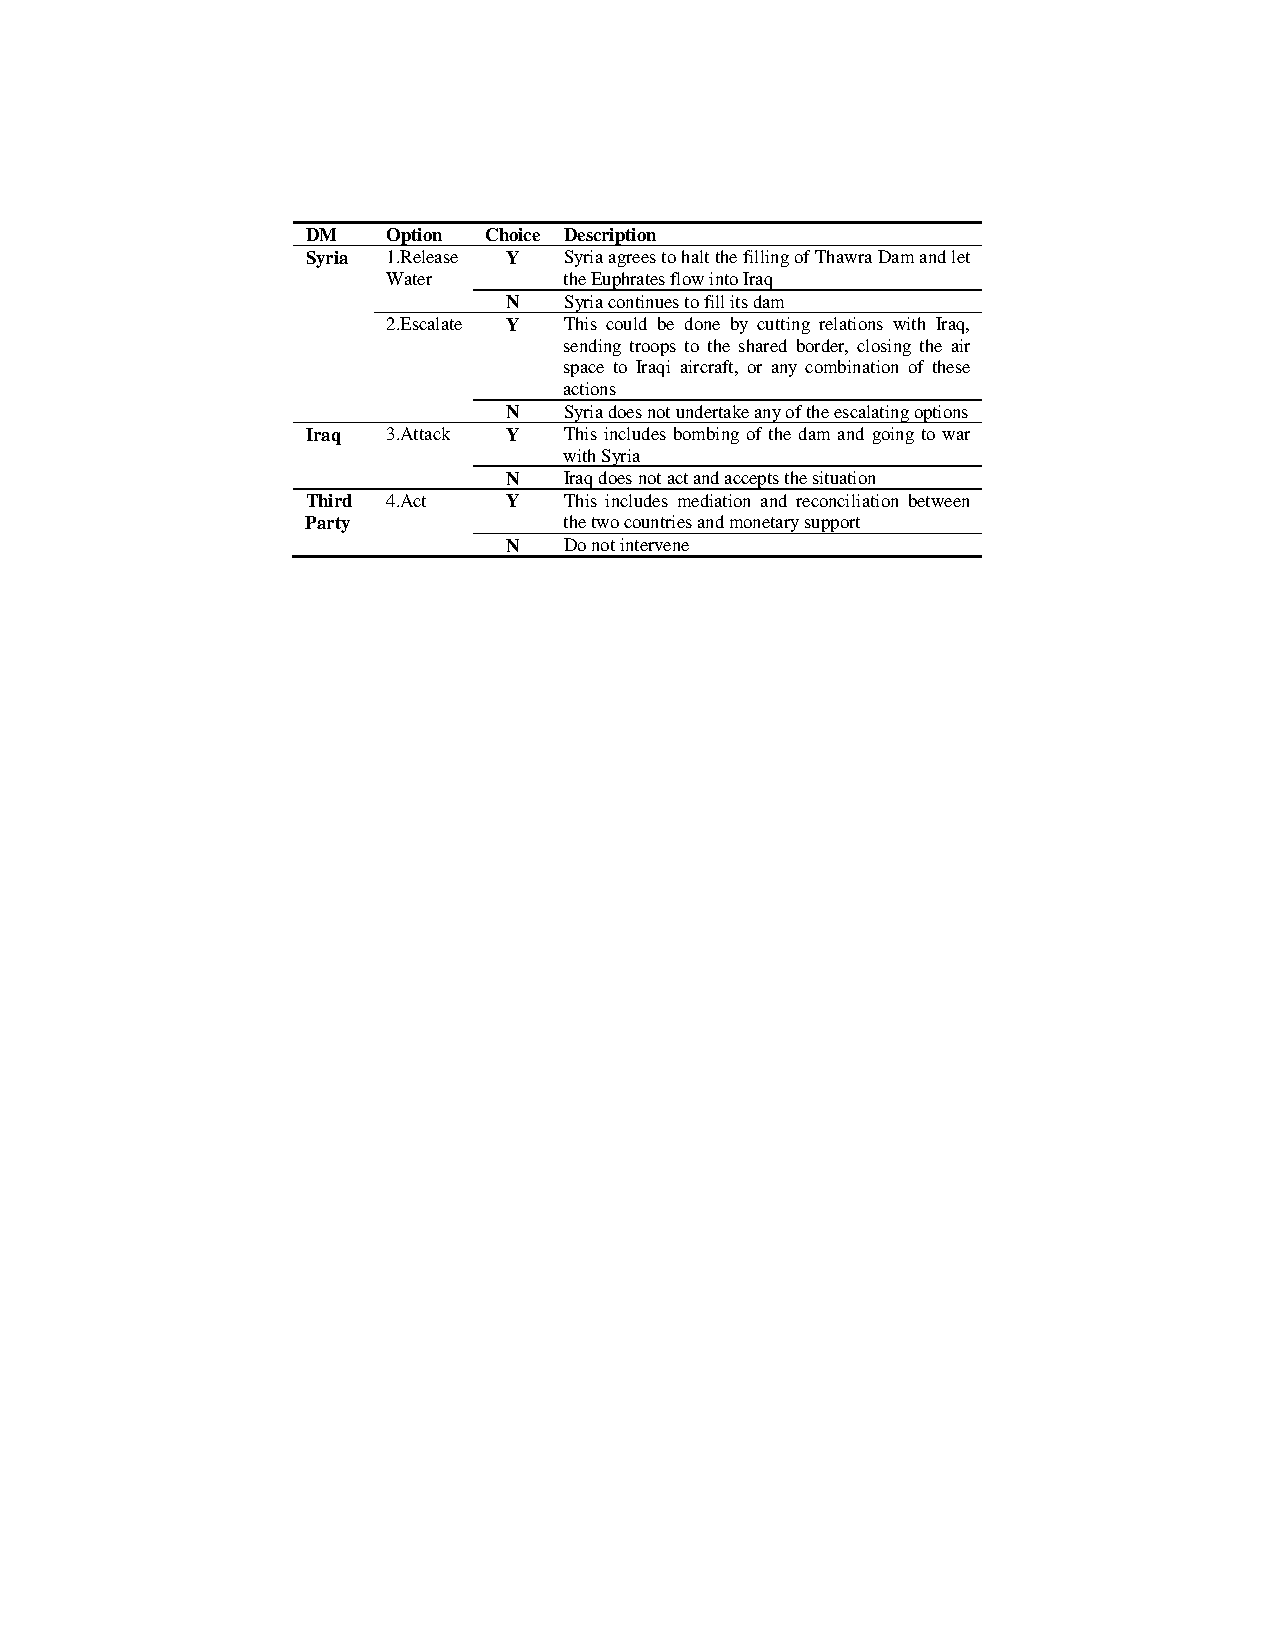
\includegraphics[scale=1]{PDF-IMG/tables/1.pdf}

\caption{DMs, options and descriptions for the 1975 conflict}

\label{tbl:t1}
\end{table}

To emphasize the effect of the third party, this conflict will be analyzed without and with the intervention of the third party. The sets of possible states are given in Tables \ref{tbl:t2} and \ref{tbl:t3}, respectively. Notice that there is one infeasible situation in which Syria both releases the water and escalates the situation at the same time (mutually exclusive options). Taking this into account resulted in the removal of two states in the model without the intervention of the third party and the removal of four states in the model with the participation of the third party.

\begin{table}[H]
\centering
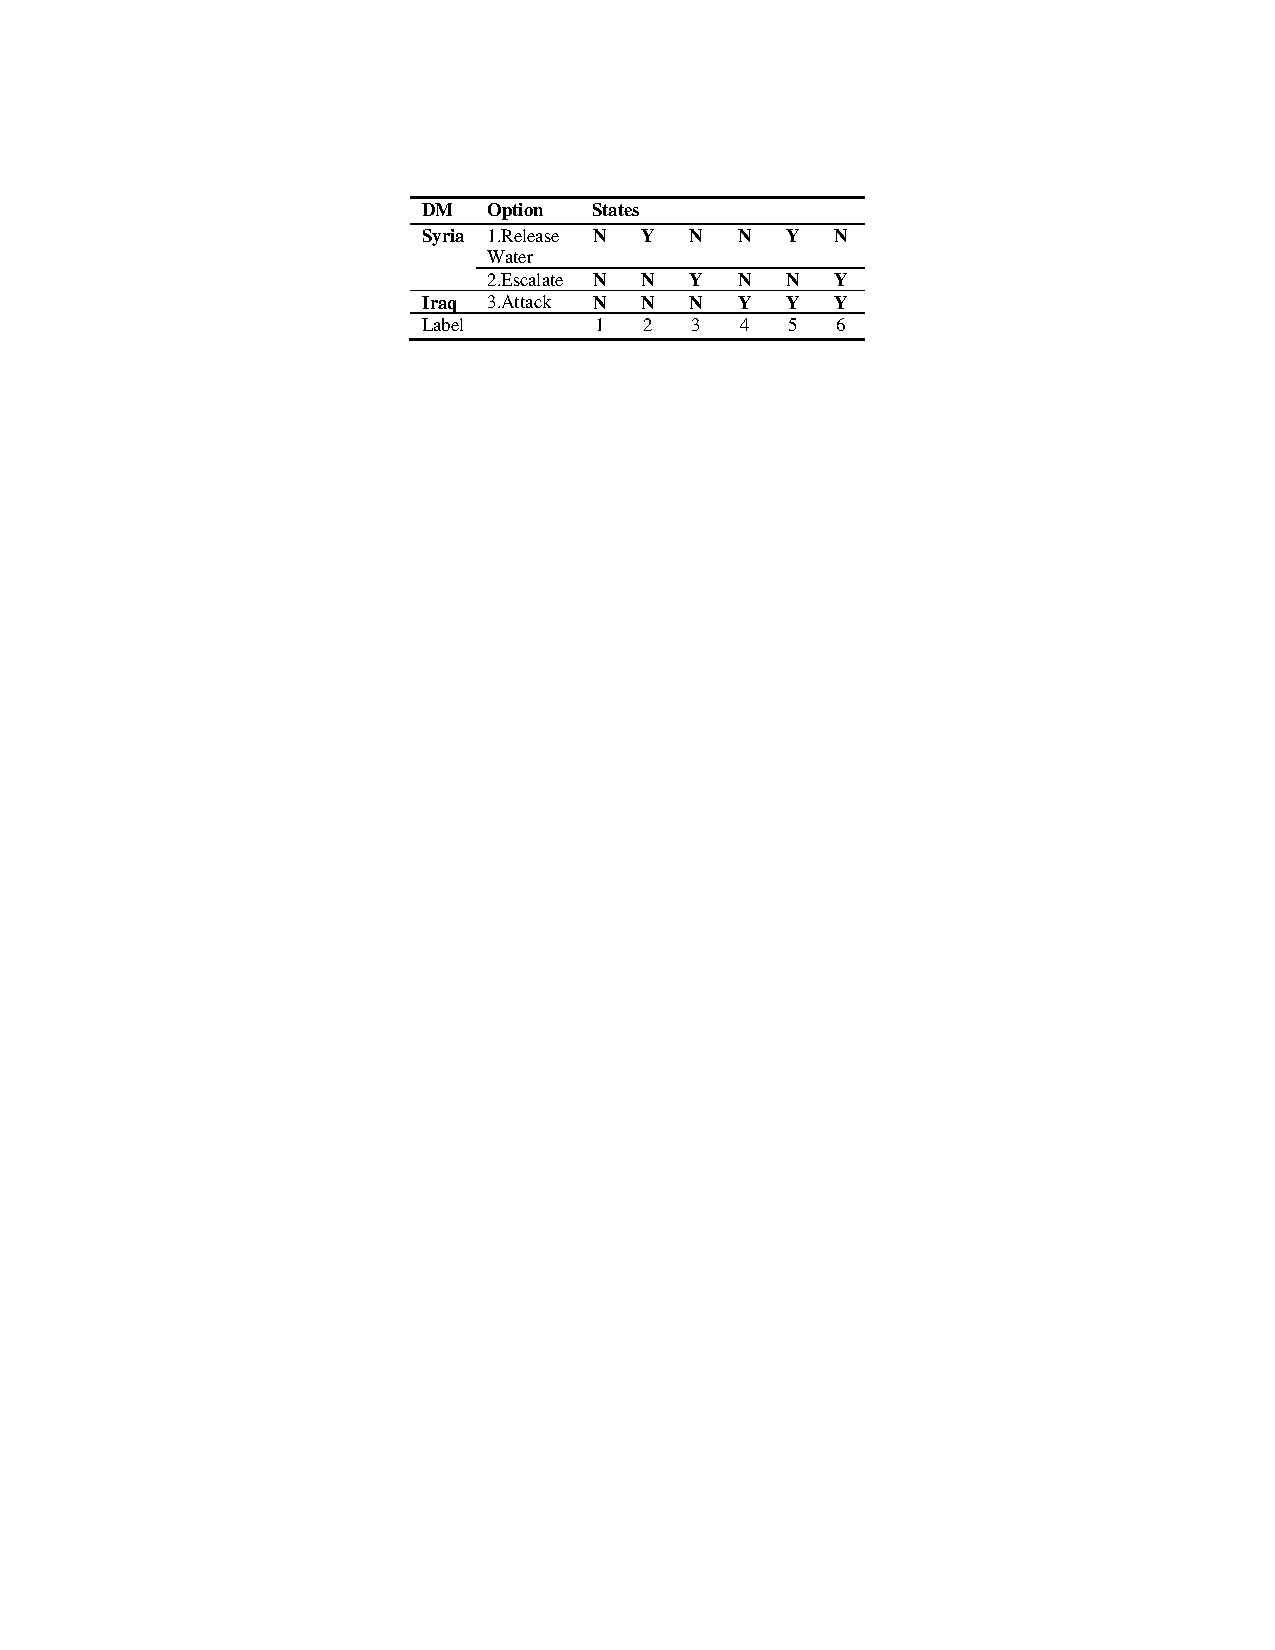
\includegraphics[scale=1]{PDF-IMG/tables/2.pdf}

\caption{DMs, options and states for the 1975 conflict without the third party}

\label{tbl:t2}
\end{table}

\begin{table}[H]
\centering
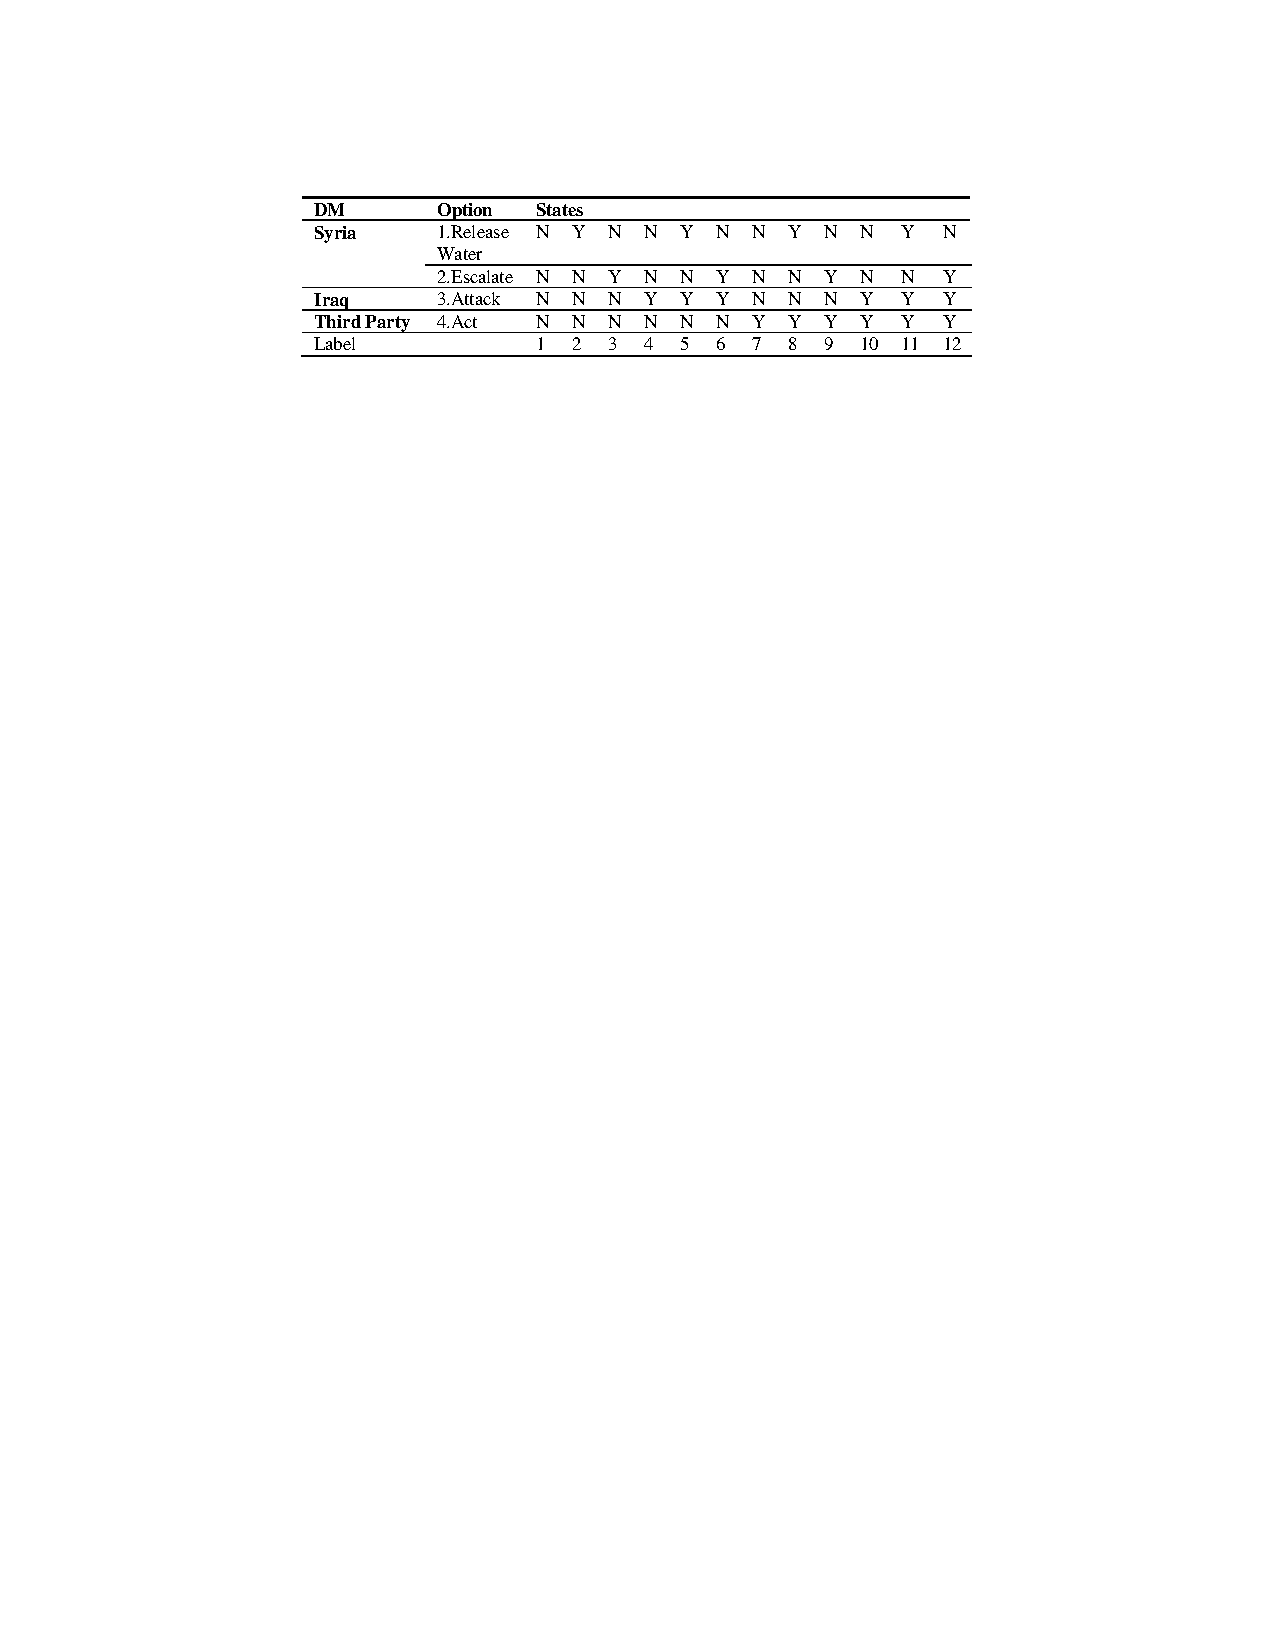
\includegraphics[scale=1]{PDF-IMG/tables/3.pdf}

\caption{DMs, options and states for the 1975 conflict with the third party}

\label{tbl:t3}
\end{table}

Figures \ref{fig:IrSyGM} and \ref{fig:IrSyGM2} show the integrated Graph Model of the conflict both without and with the participation of the third party, respectively. The numbers in the nodes refer to the state numbers as indicated in Tables \ref{tbl:t2} and \ref{tbl:t3}. The lines with arrows between the nodes are moves that can be carried out by the indicated DM in one step. 

\begin{center}
\begin{figure}[H]
\centering
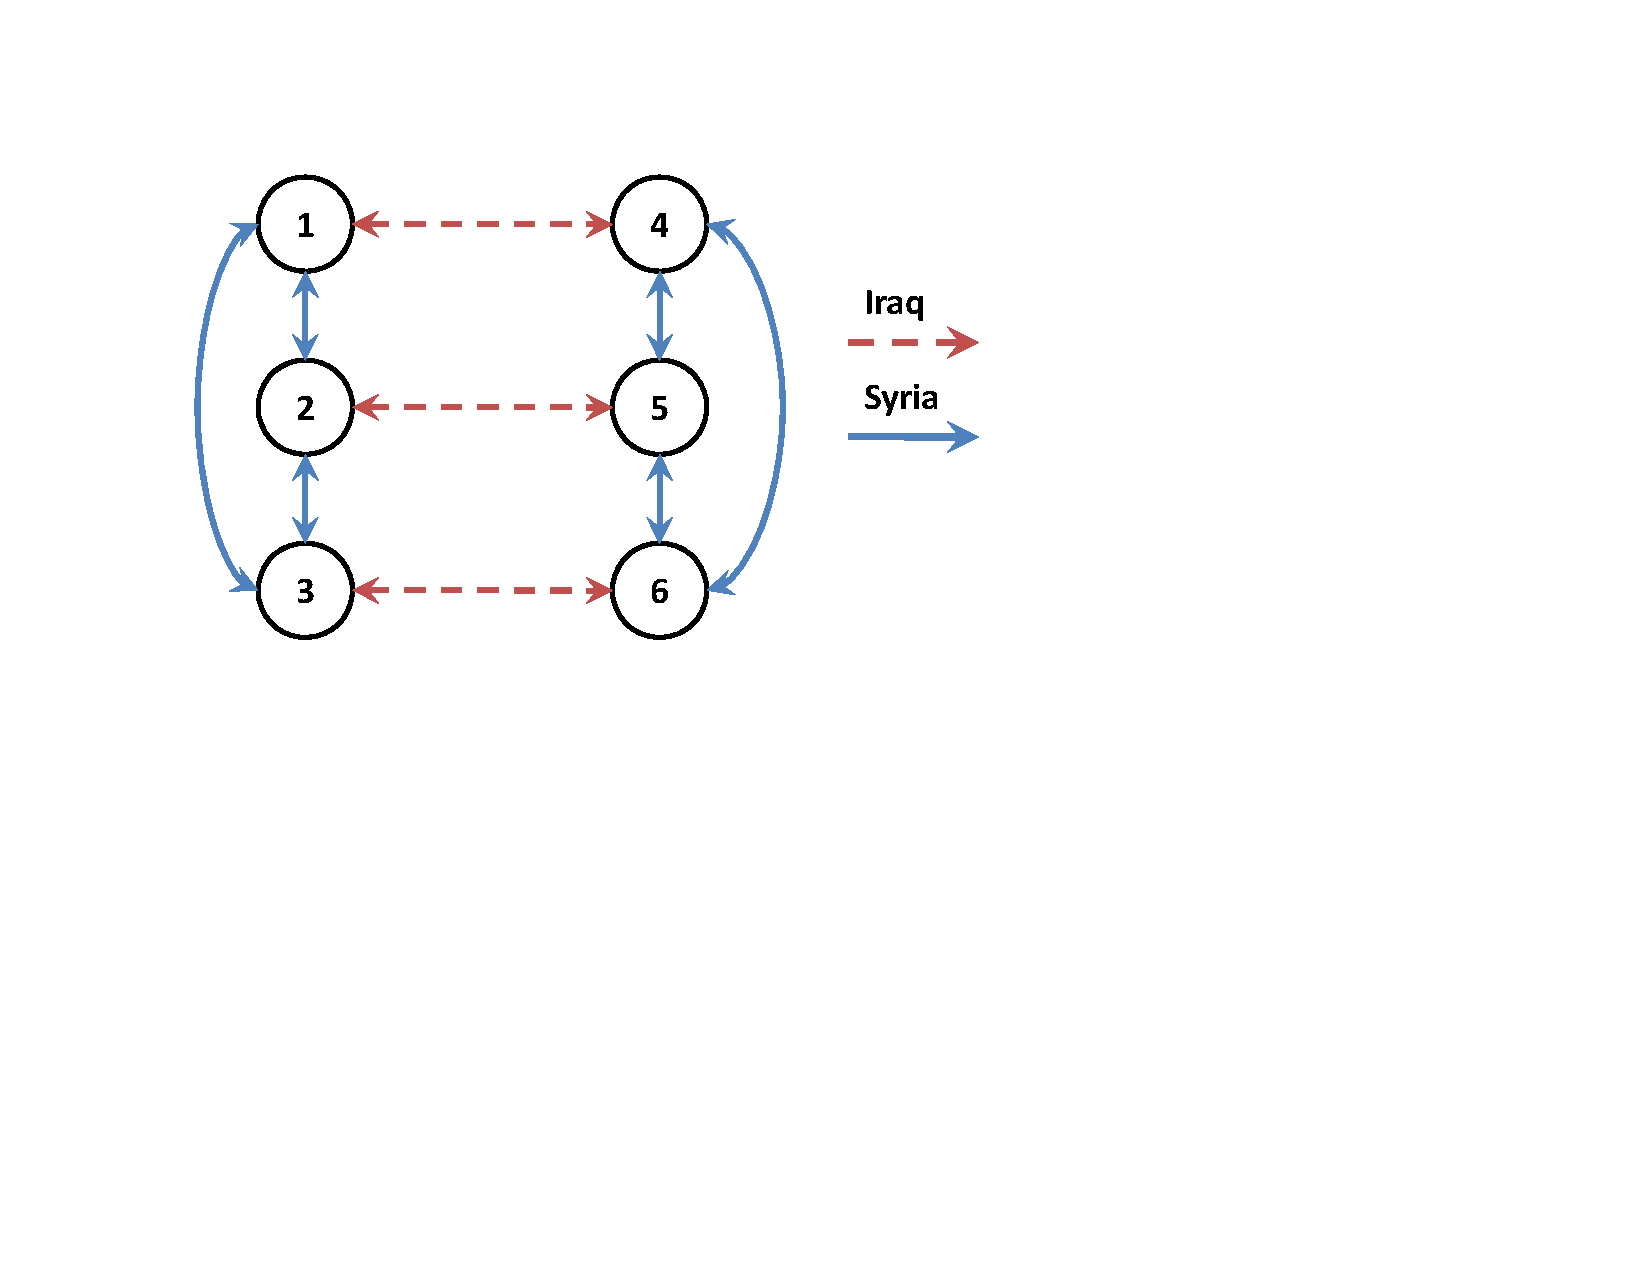
\includegraphics[scale=0.6]{PDF-IMG/IrSy1.pdf}

\caption{Integrated Graph Model of the 1975 conflict without the third party}

\label{fig:IrSyGM}
\end{figure}
\end{center}

\begin{center}
\begin{figure}[H]
\centering
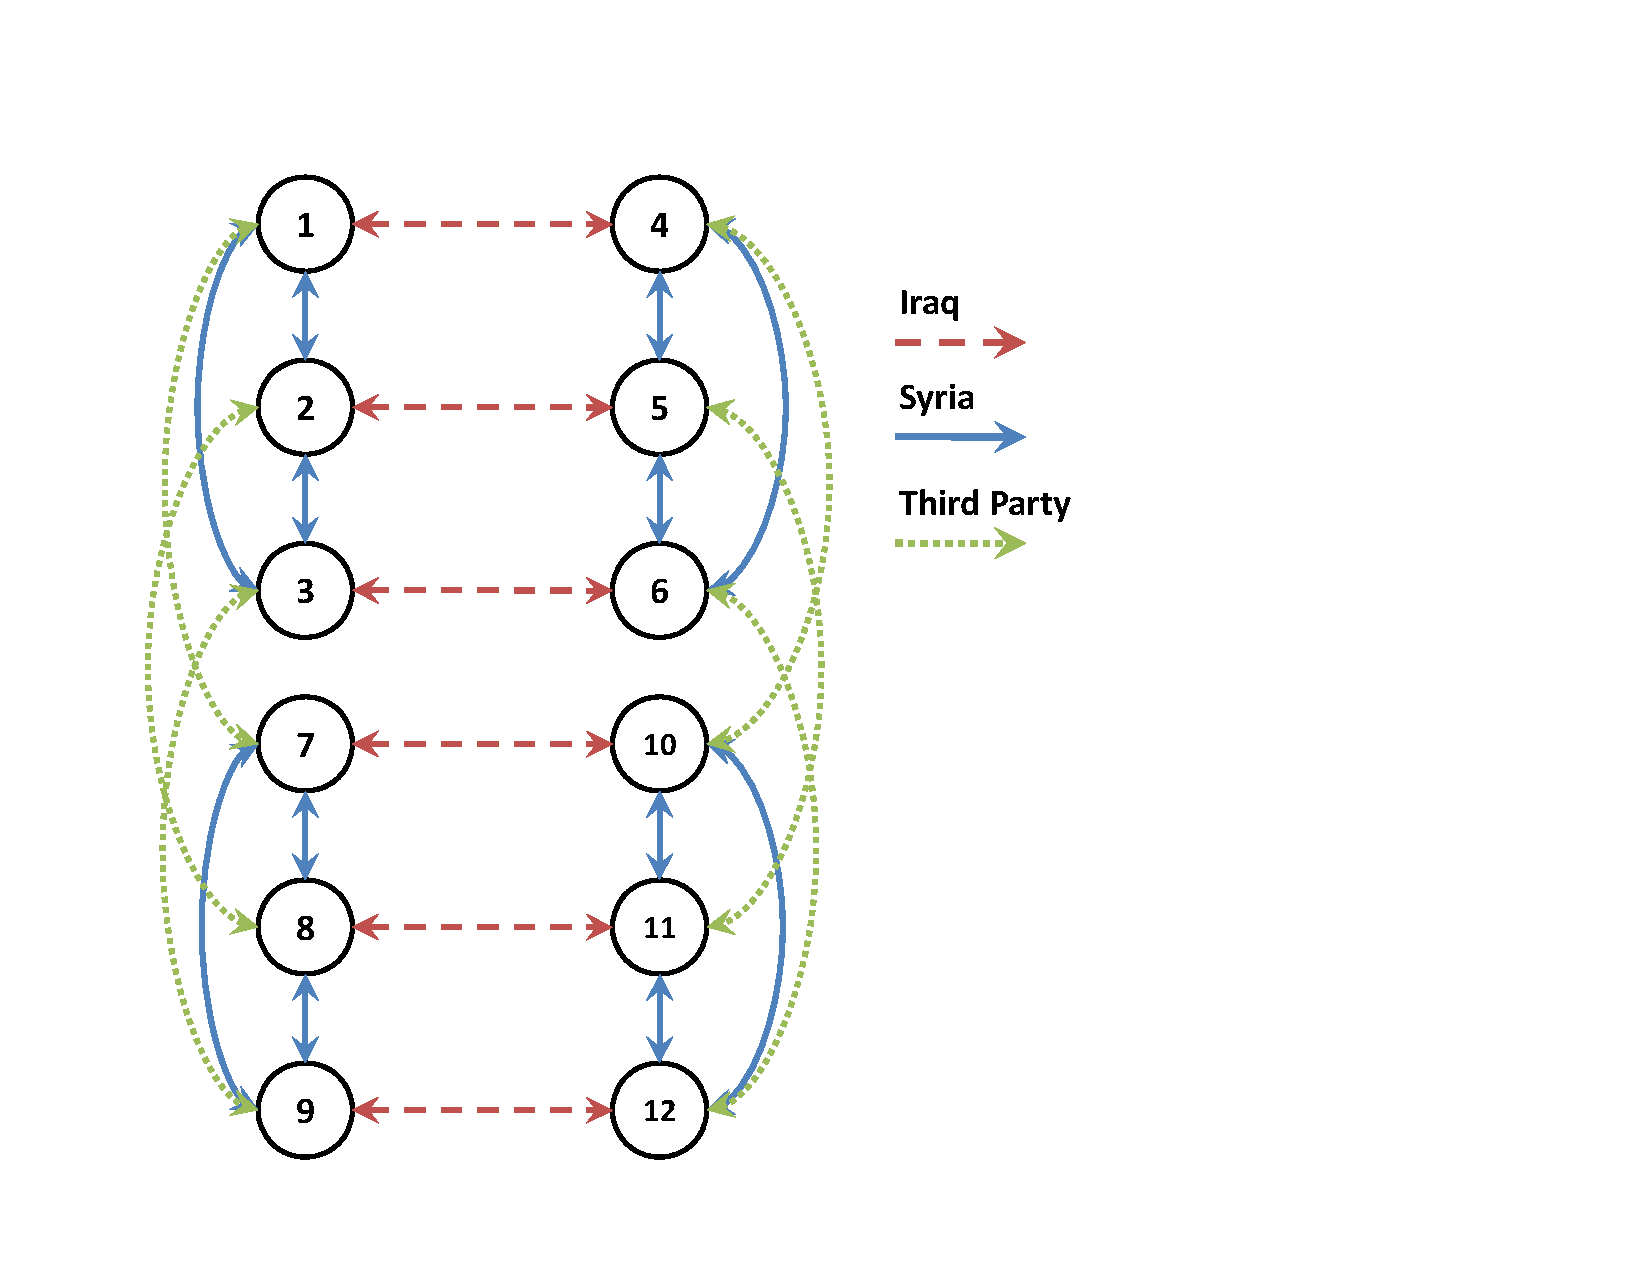
\includegraphics[scale=0.5]{PDF-IMG/IrSy2.pdf}

\caption{Integrated Graph Model of the 1975 conflict with the third party}

\label{fig:IrSyGM2}
\end{figure}
\end{center}

Table \ref{tbl:t4} presents the preference prioritization information for each DM in the 1975 conflict without the participation of the third party, from most important at the top to least important at the bottom for each DM. The statements presented herein are a sample of how the ranking of states is constructed. This information is used to order the states from most to least preferred by the DM. Assuming transitivity for the preferences, Table \ref{tbl:t5} presents the ranking of states from most to least preferred for both Syria and Iraq using option prioritization \citep{hipel1997decision,fang2003a,fang2003b}. For example, State 1, which is the status quo, is the best state to be in for Syria. State 5, in which Syria releases the Euphrates and Iraq attacks at the same time, is considered the worst possible state for Syria.

\begin{table}[H]
\centering
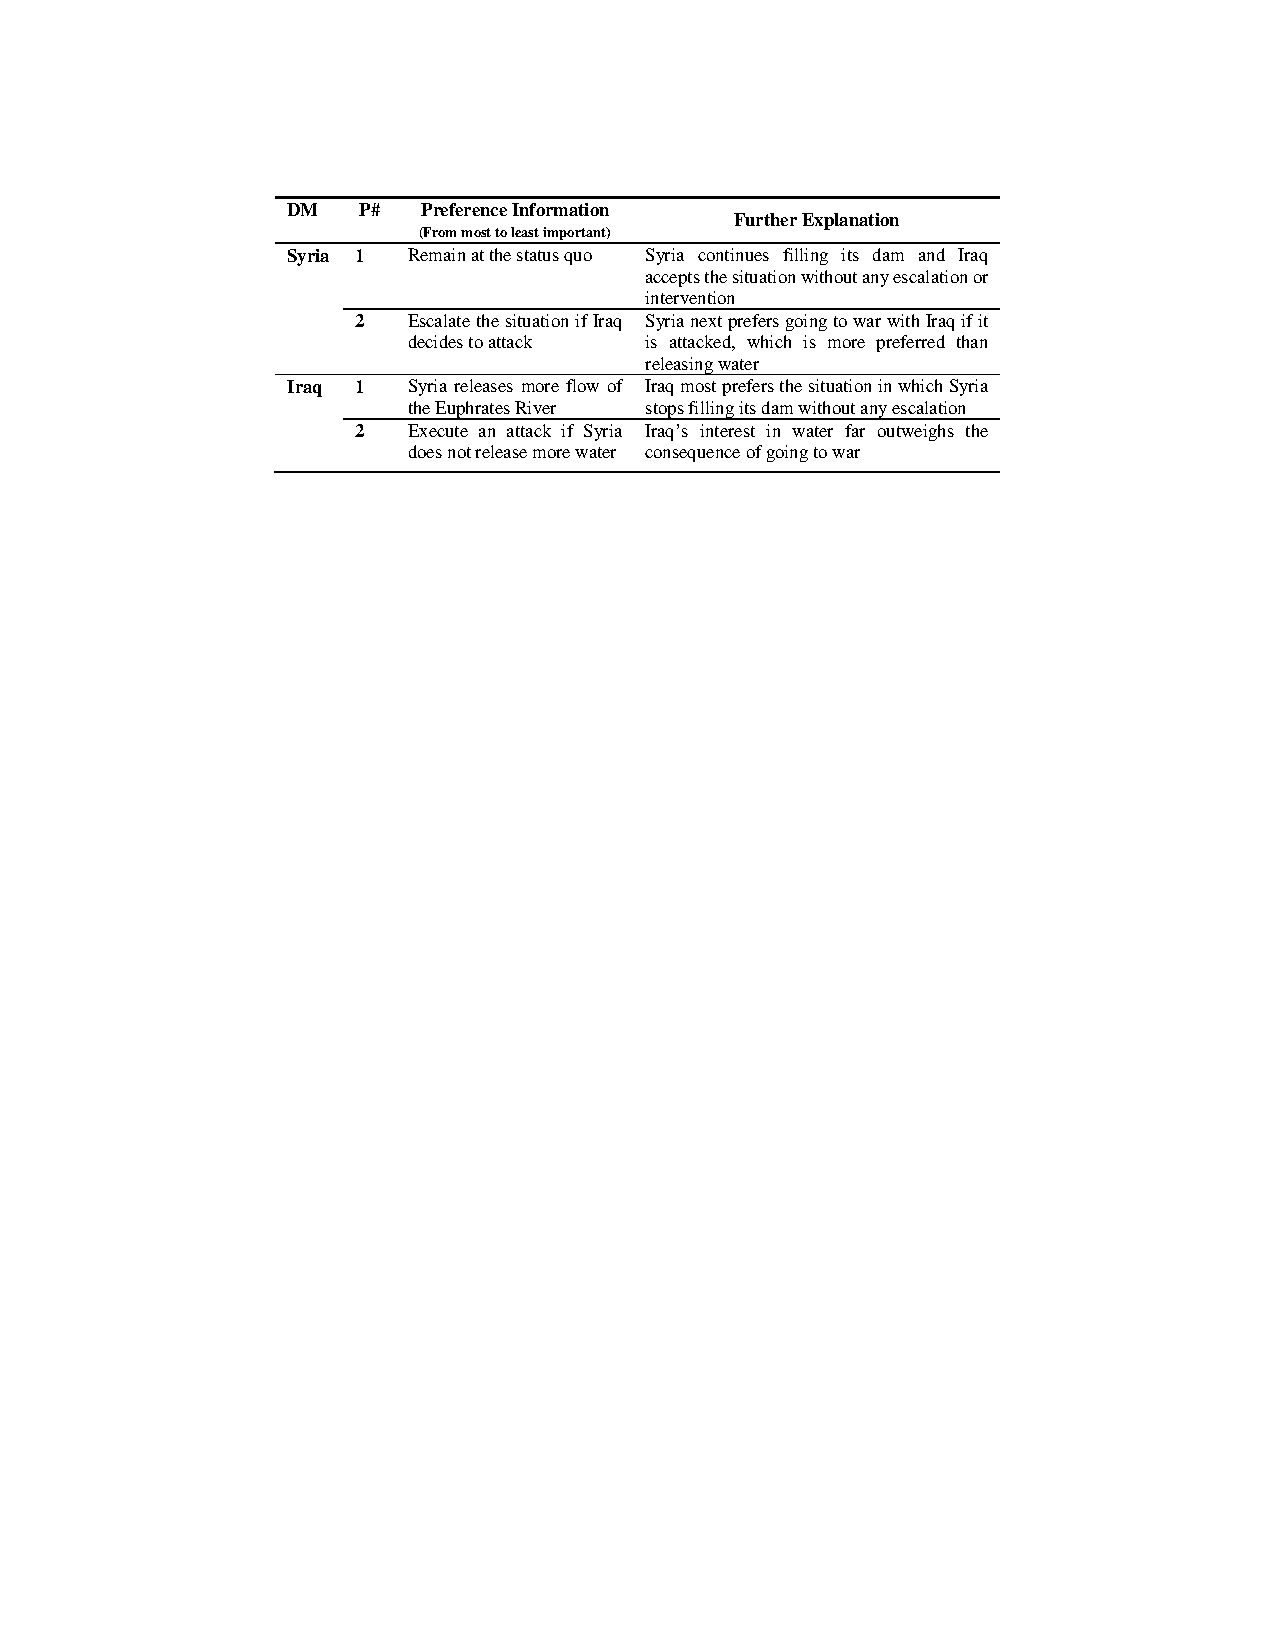
\includegraphics[scale=1]{PDF-IMG/tables/4.pdf}

\caption{Preference prioritization information for the 1975 conflict without the third party}

\label{tbl:t4}
\end{table}


\begin{table}[H]
\centering
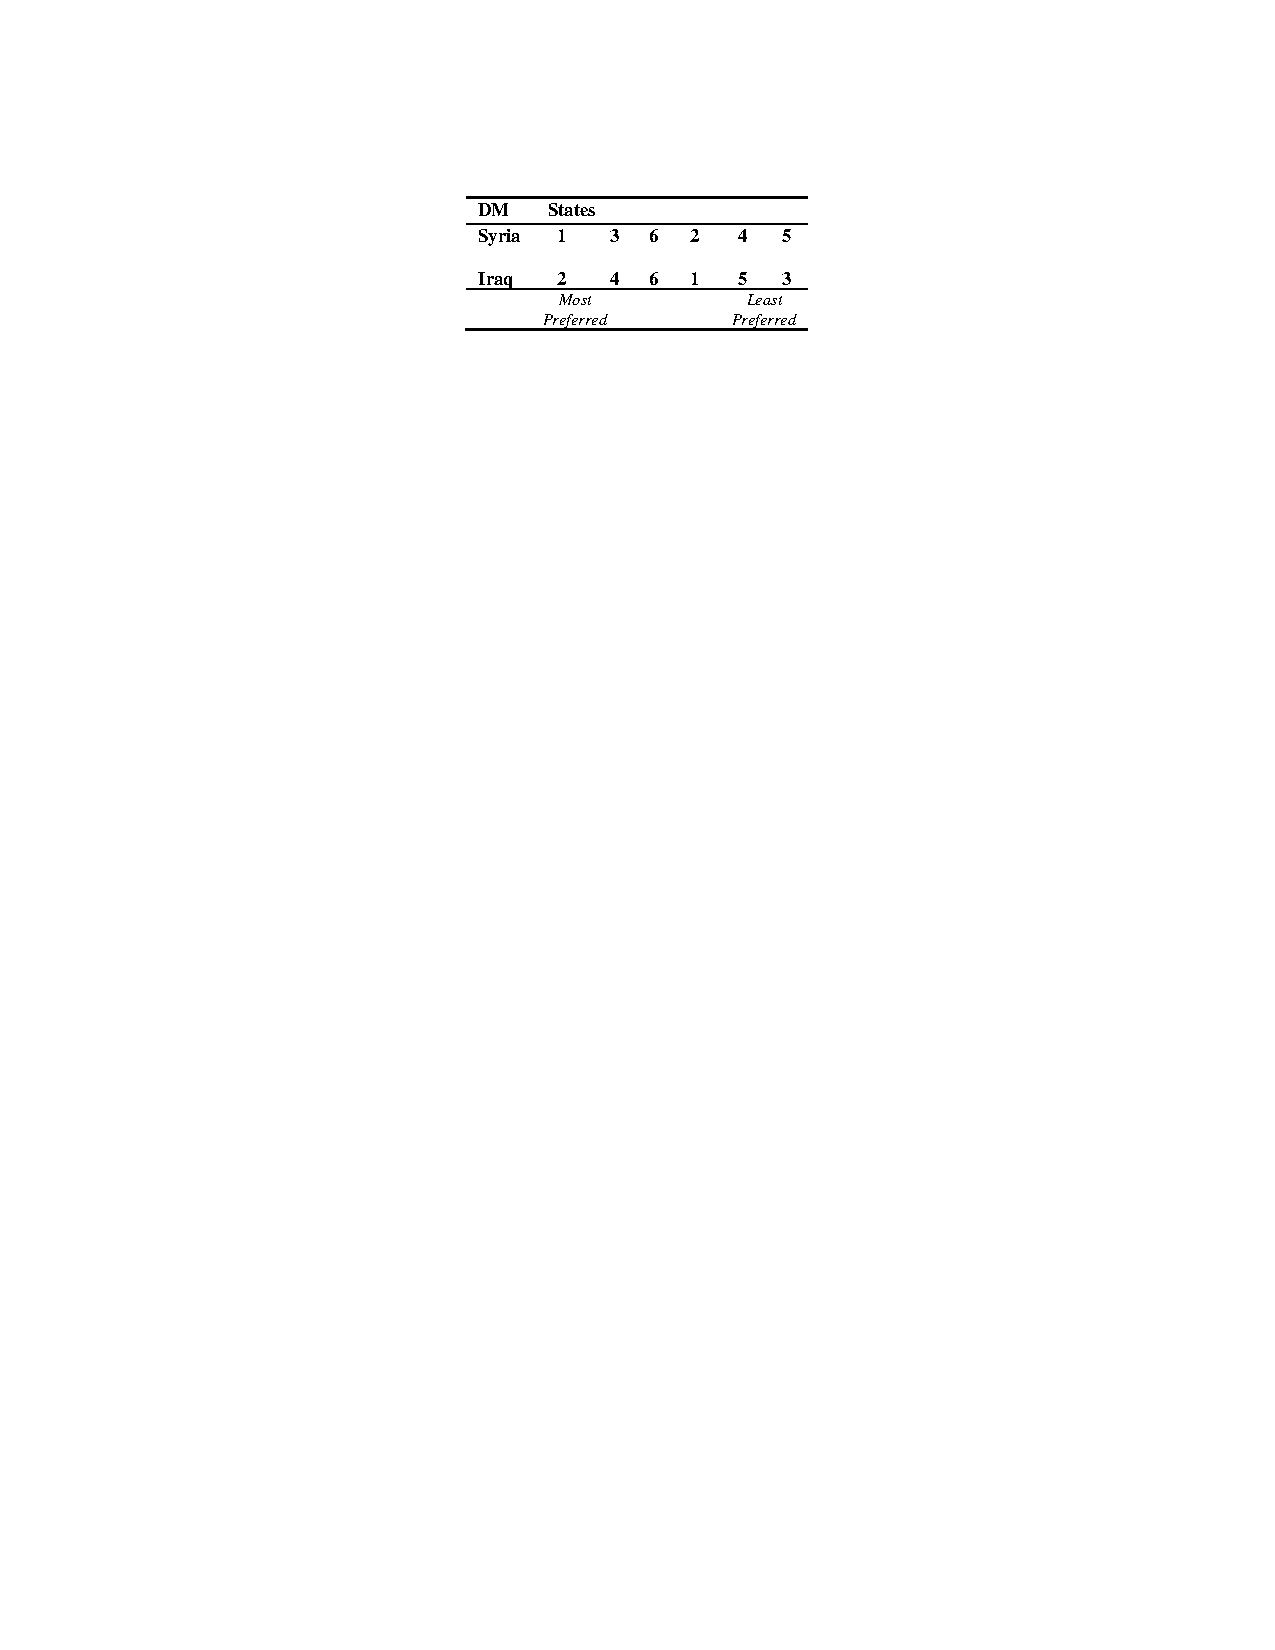
\includegraphics[scale=1]{PDF-IMG/tables/5.pdf}

\caption{Ranking of states for the DMs in the 1975 conflict without the third party}

\label{tbl:t5}
\end{table}

The third party could be viewed as an actual DM if it has its own options and preferences. However, if the party is not an actual stakeholder in the conflict but is motivated to bring about a more preferred equilibrium, then it can be categorized as Arbitrator, Coordinator or Donor \citep{sakamoto2005}. If the party has the influence to change other DMs' preferences or options, then the party is called a Donor. On the other hand, if the party has the power to exclude some states, then it is considered to be an Arbitrator. In this conflict, the third party, Saudi Arabia, is clearly a Donor as it contributed to financing the basin development and both DMs, Syria and Iraq, want to please Saudi Arabia. Therefore, DMs' preferences, especially on the part of Syria, are changed. Table \ref{tbl:t6} presents the preference prioritization information for each DM in the 1975 conflict with the participation of the third party from most to least preferred. Table \ref{tbl:t7} gives the preferences for Syria, Iraq, and the third party from most to least preferred.

\begin{table}[H]
\centering
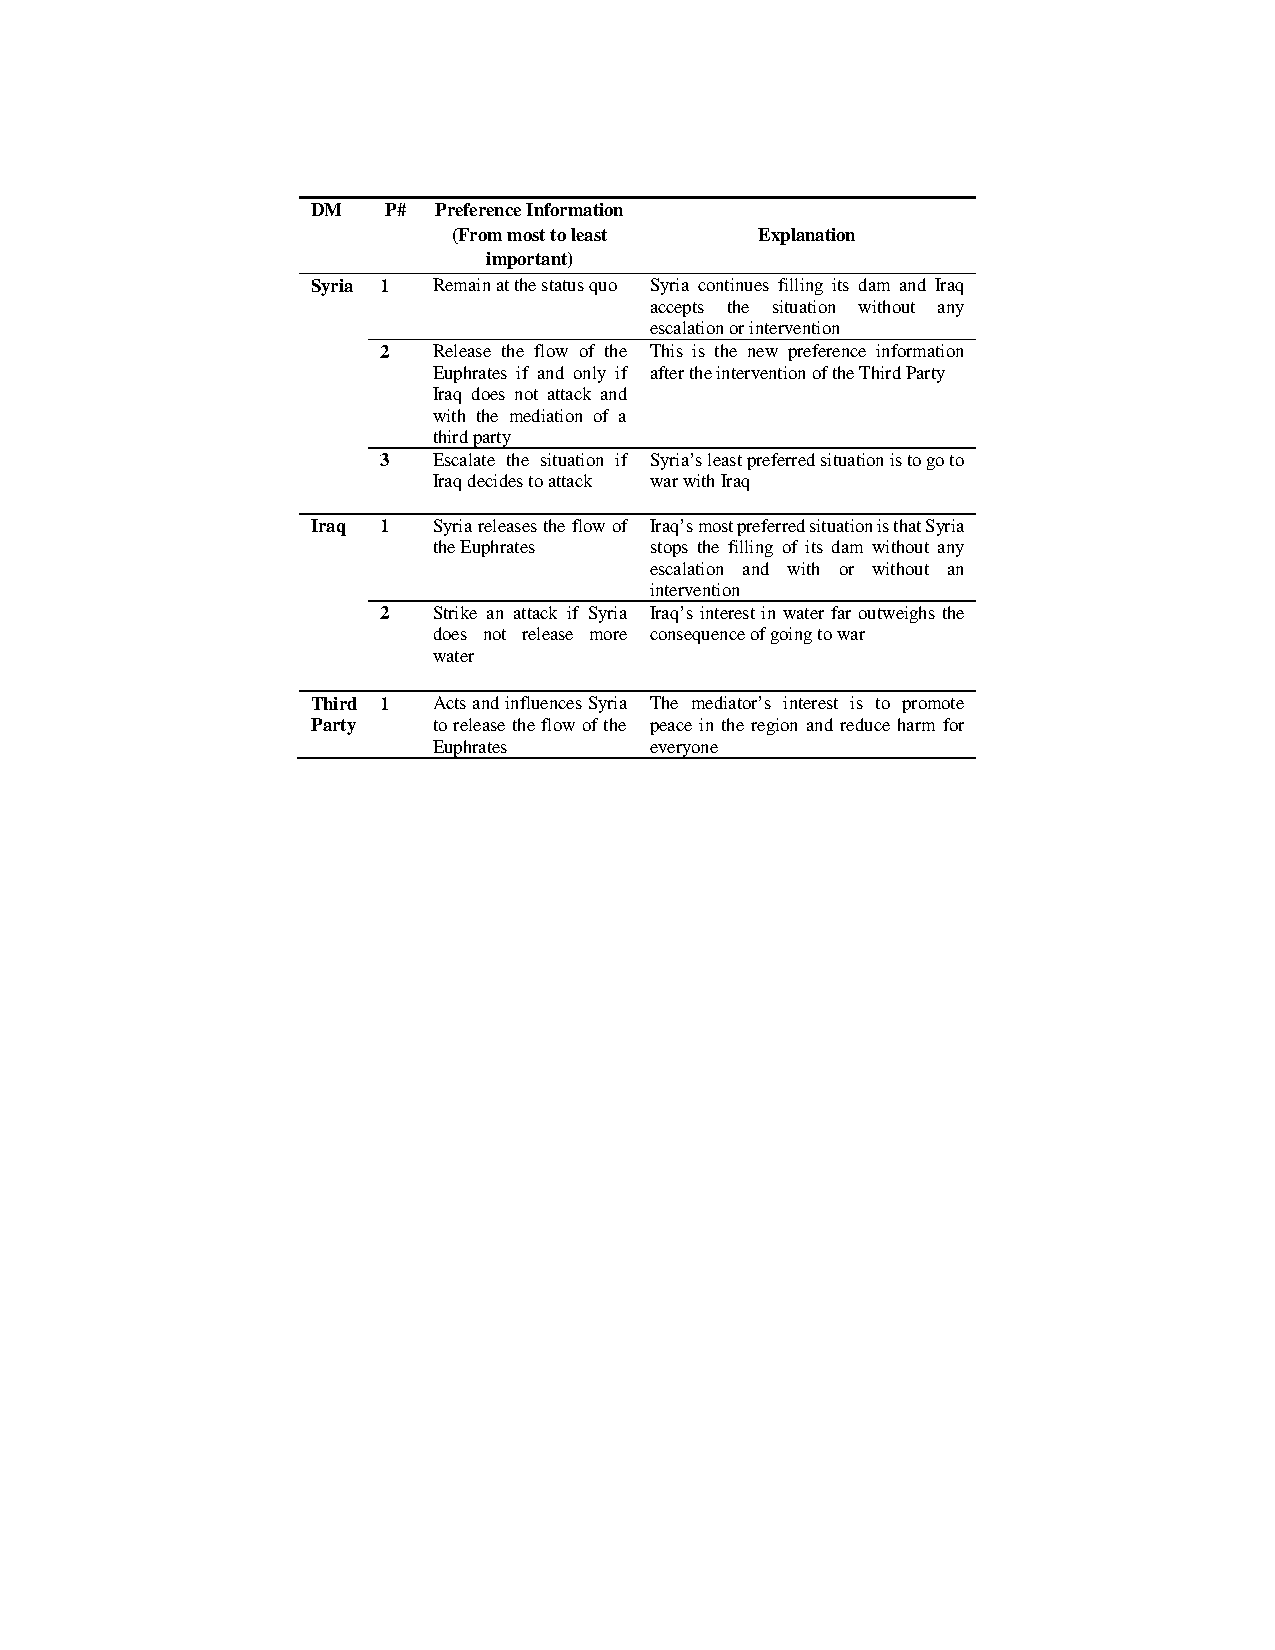
\includegraphics[scale=1]{PDF-IMG/tables/6.pdf}

\caption{Preference prioritization information for the 1975 conflict with the third party}

\label{tbl:t6}
\end{table}

\begin{table}[H]
\centering
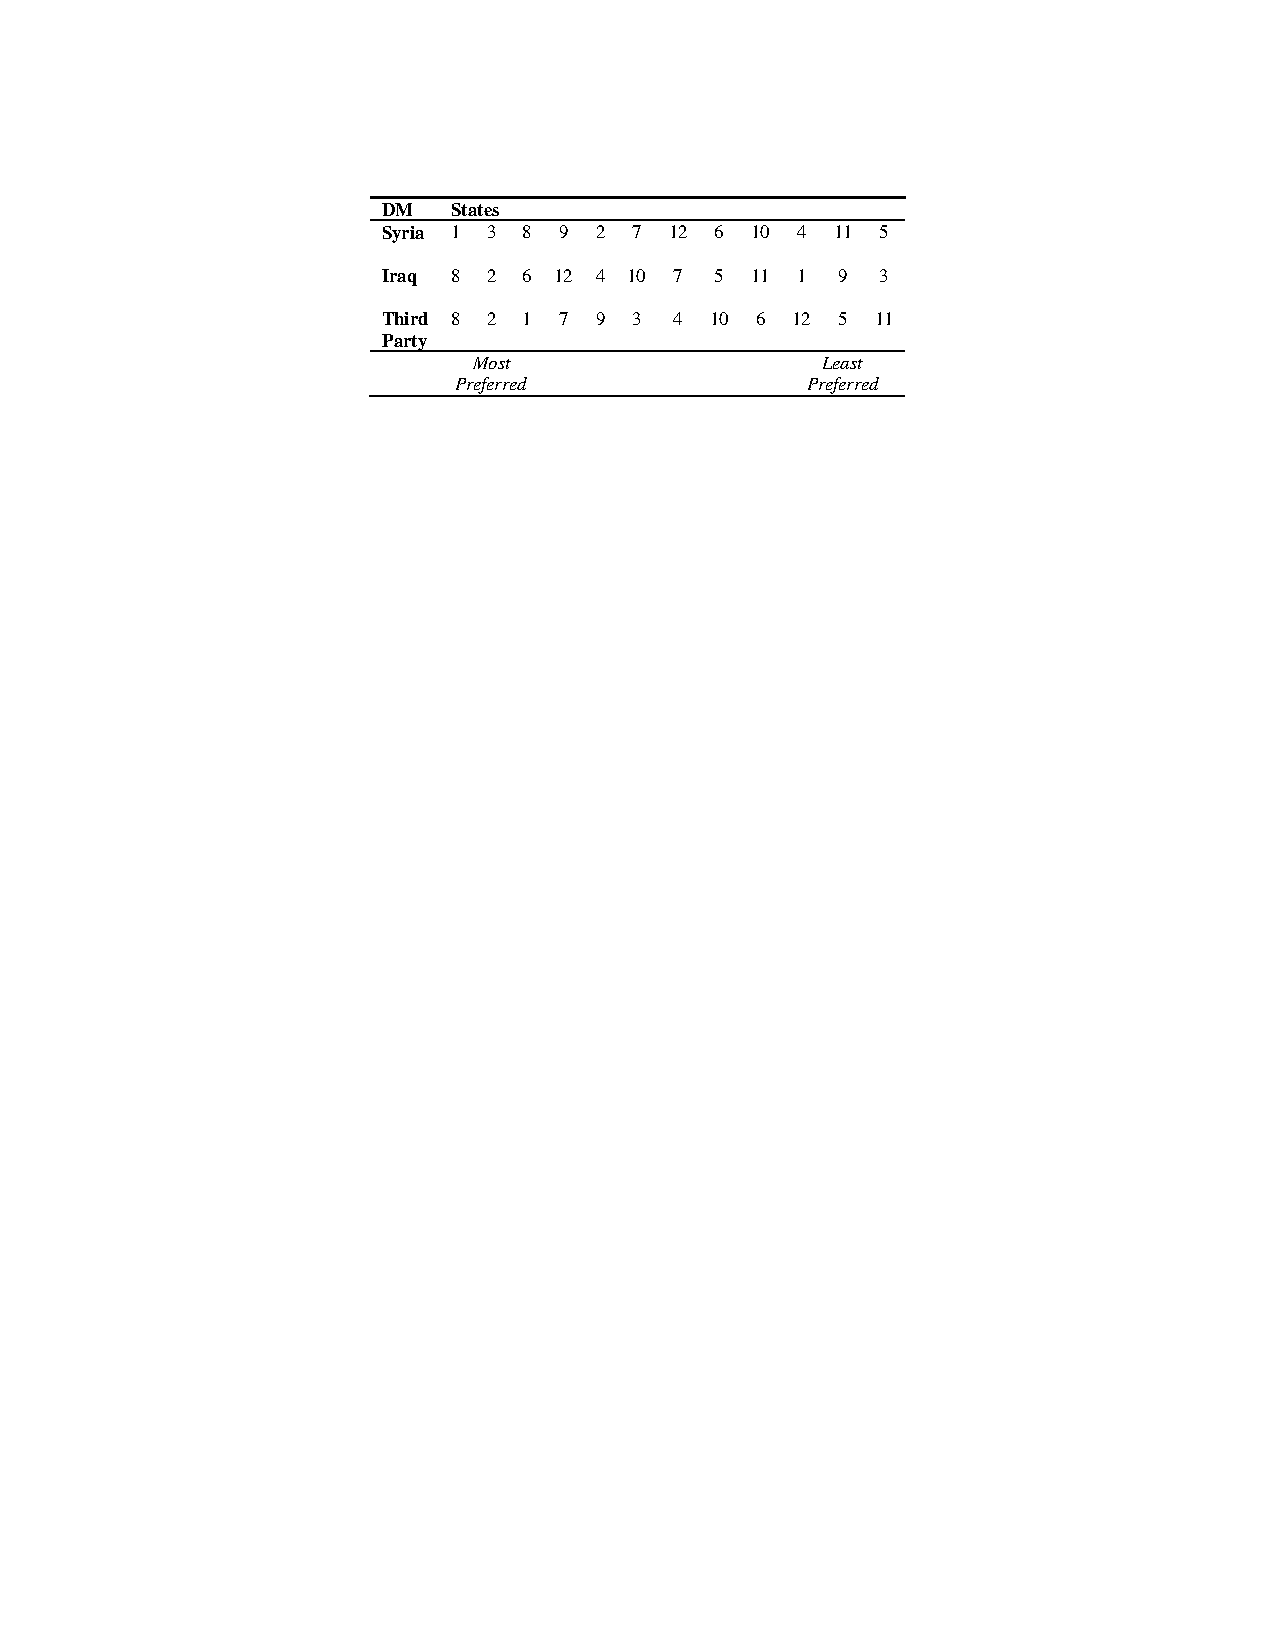
\includegraphics[scale=1]{PDF-IMG/tables/7.pdf}

\caption{Ranking of states for the DMs in the 1975 conflict with the third party}

\label{tbl:t7}
\end{table}

The objective of the analysis is to determine the equilibrium states, which are the states from which no DM is motivated to move and, therefore, the conflict will probably end at that particular state. To determine the equilibrium states we use stability definitions (or solution concepts), which describe human behavior and patterns based on moves and counter moves. Equilibria are states that are stable for all DMs. After inputting the foregoing information into the decision support system GMCR II, equilibrium results are obtained for both Syria and Iraq without the third party (Table \ref{tbl:t8}) and with the third party (Table \ref{tbl:t9}). Restricting Iraq's alternative of attacking does not affect the equilibria for both cases. In Tables \ref{tbl:t8} and \ref{tbl:t9}, the left column gives the different stability definitions while the remaining columns present the stability calculation results for each solution concept corresponding to the state. Nash and Sequential Stability (SEQ) are considered the strongest stability definitions. General Metarationality (GMR) and Symmetric Metarationality (SMR) are not considered as strong stability definitions since DMs are permitted to harm themselves during the process of sanctioning. \citet{Fang1989} discuss the relationships among the different solution concepts.

\begin{table}[H]
\centering
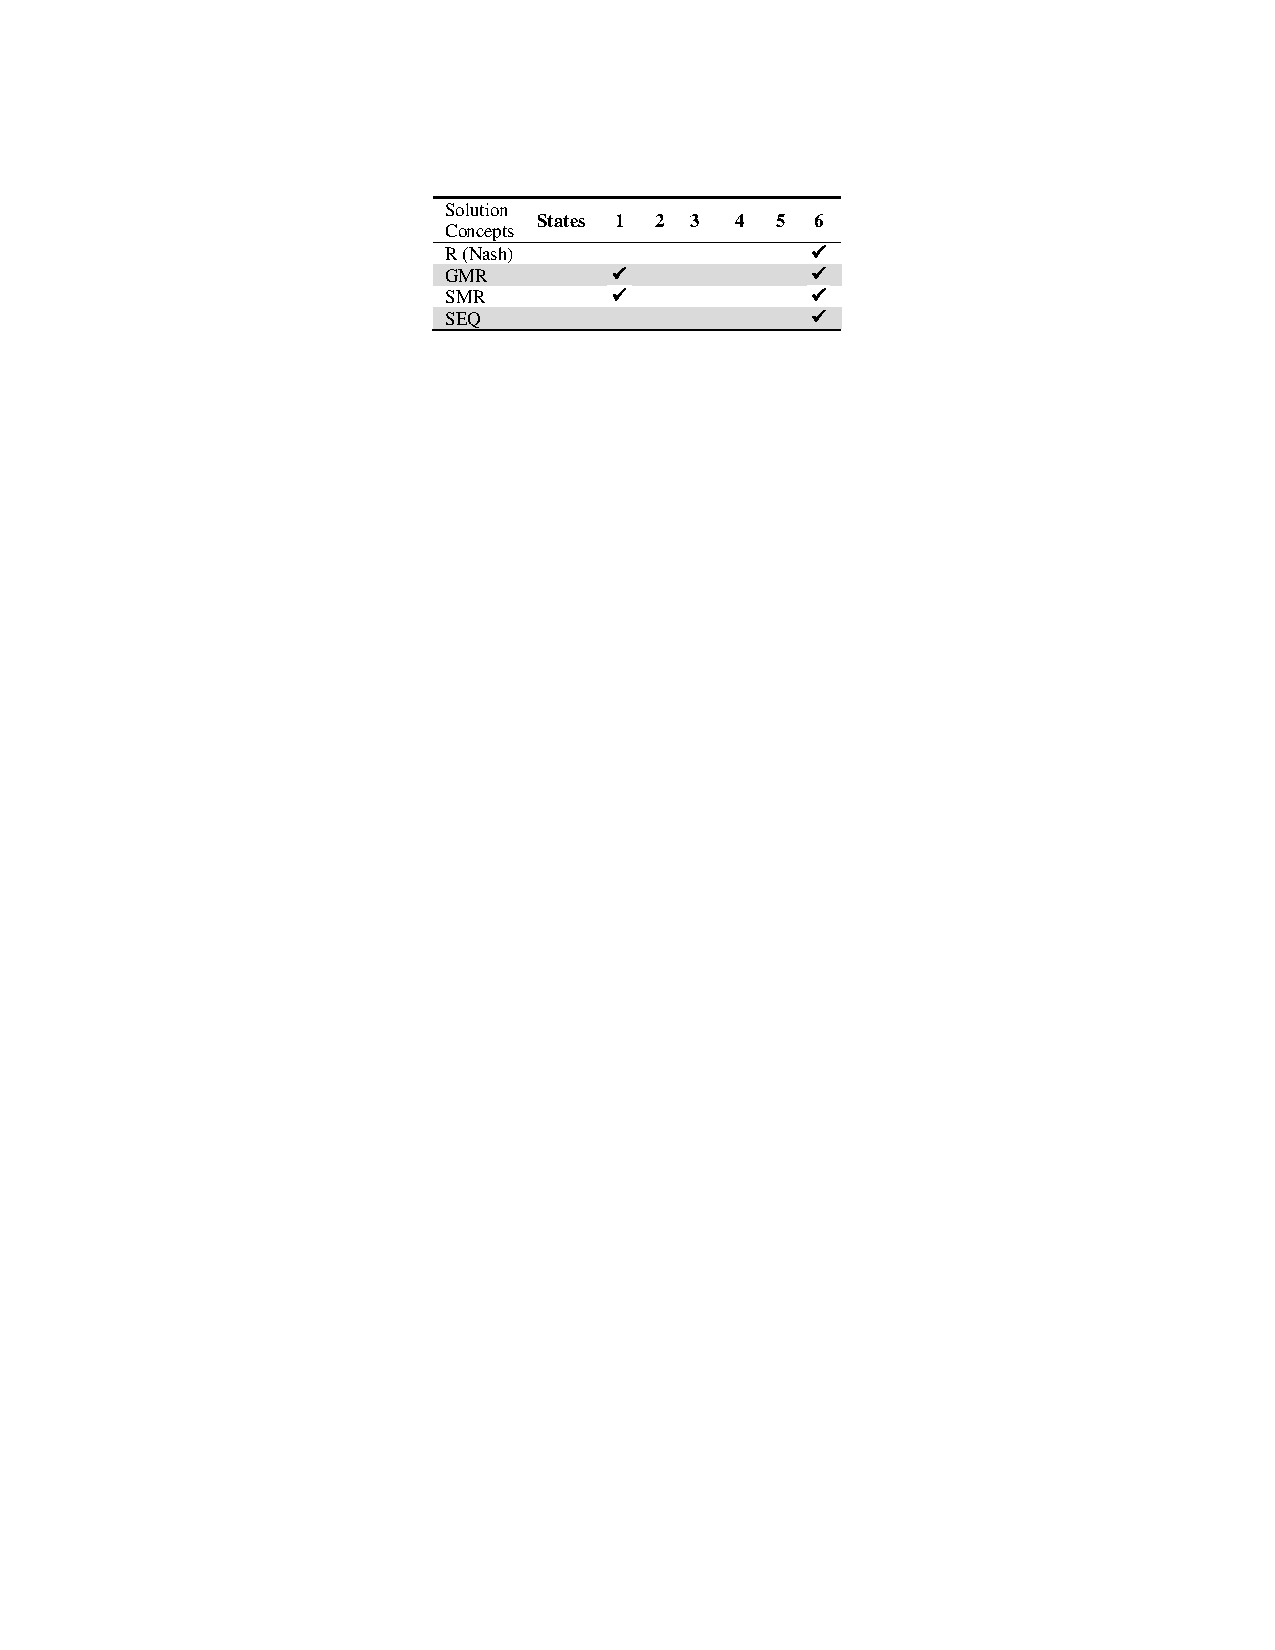
\includegraphics[scale=1]{PDF-IMG/tables/8.pdf}

\caption{Equilibrium results for the 1975 conflict without the third party}

\label{tbl:t8}
\end{table}

\begin{table}[H]
\centering
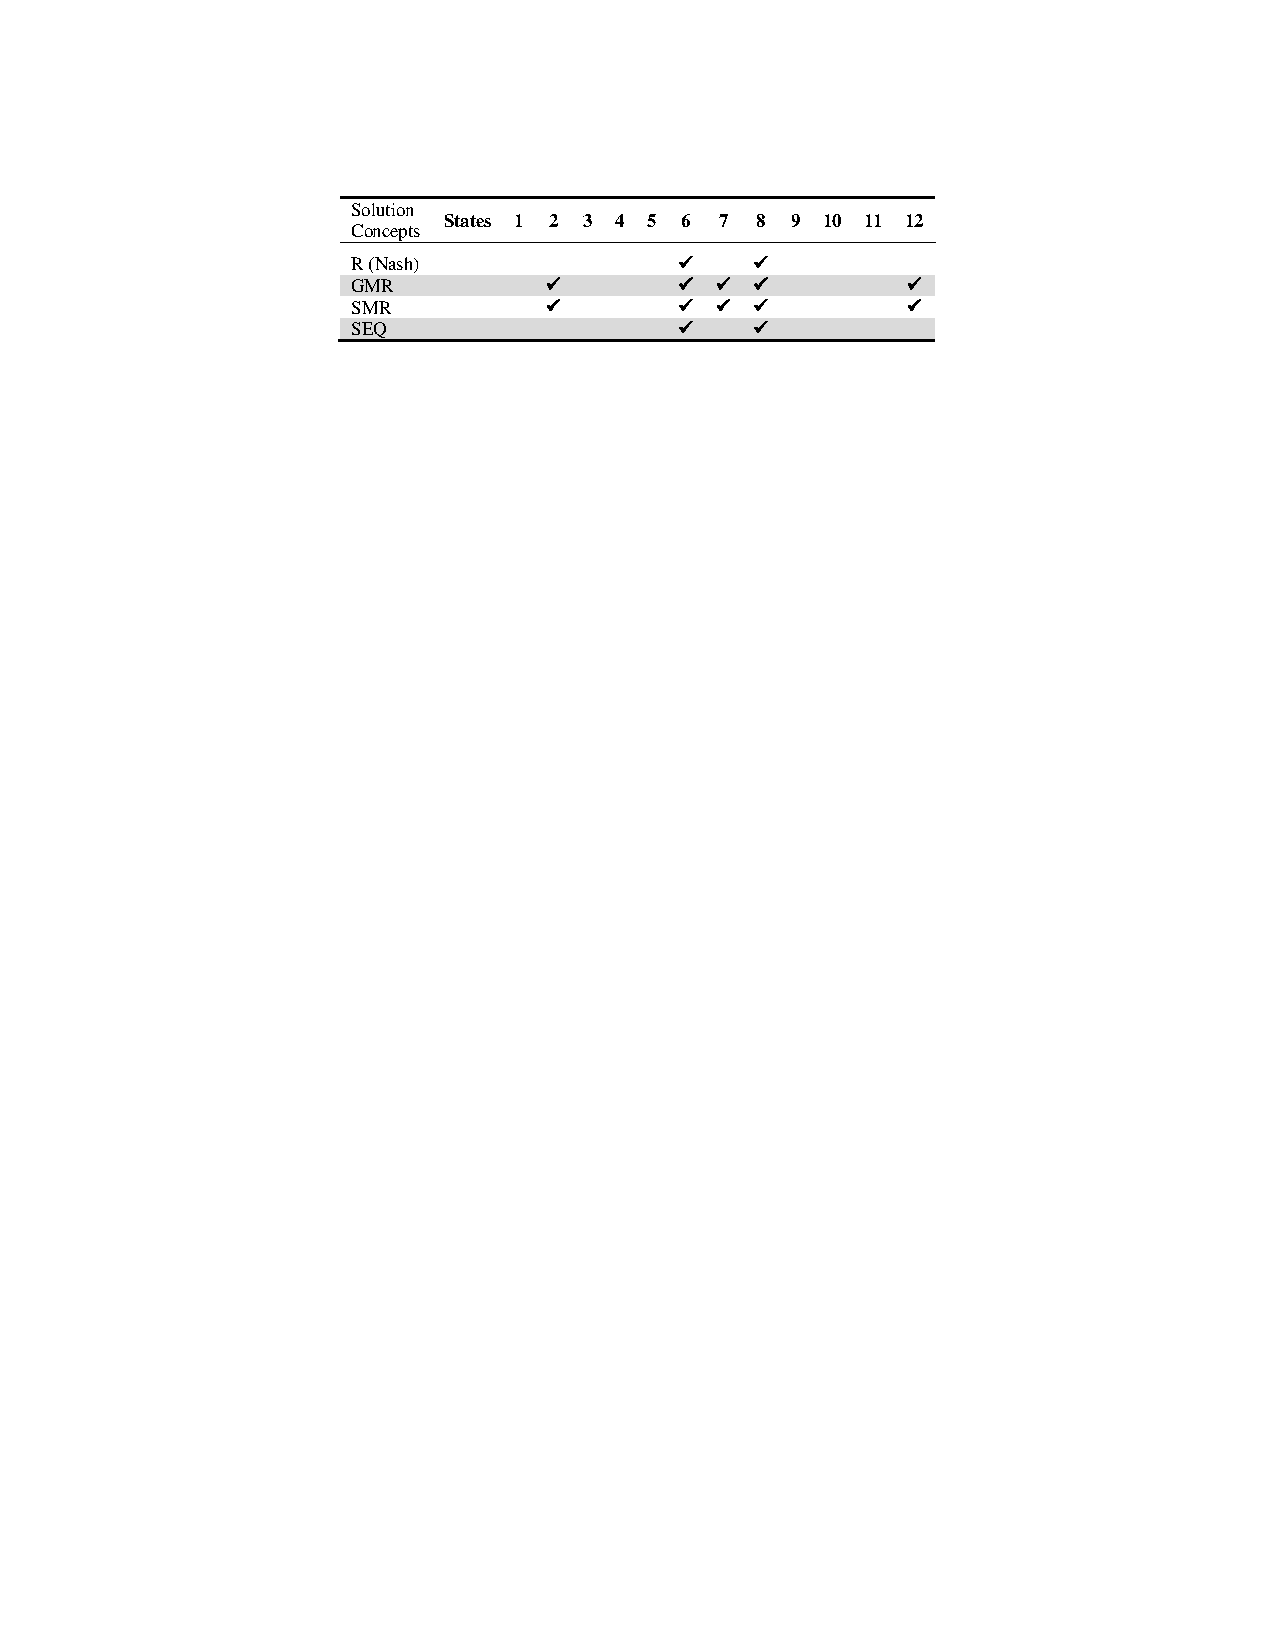
\includegraphics[scale=1]{PDF-IMG/tables/9.pdf}

\caption{Equilibrium results for the 1975 conflict with the third party}

\label{tbl:t9}
\end{table}

It is clear from the aforementioned analysis that when the third party does not participate (Table  \ref{tbl:t8}), the strongest equilibrium is state 6 which means that both Syria and Iraq go to war. And that is what nearly happened as both countries amassed their troops on their shared border. The status quo, State 1, is a very weak equilibrium and the unilateral improvement by Iraq will most likely be taken; that is, Iraq will move to state 4 in which it will attack. In contrast, with the intervention of the third party, a new equilibrium is introduced: State 8 in which Syria releases water and no escalation or attack from Iraq occurs. Referring to the ranking of states in Tables  \ref{tbl:t5} and  \ref{tbl:t7} as well as the integrated graphs in Figures \ref{fig:IrSyGM} and \ref{fig:IrSyGM2}, one can easily view the unilateral moves and improvements for each DM. A unilateral move is any possible move controlled by that particular DM, whereas a unilateral improvement necessitates that this move is also a movement to a more preferred state.  
The analysis of the conflict demonstrates how each DM's preferences may have an impact on the overall conflict. Table \ref{tbl:t10} provides the actual historical evolution of the conflict when moving from the status quo on the left via several intermediate states to the final equilibrium on the right. One can clearly see how both Syria and Iraq almost went to war until the third party intervened. It is clear that the actual historical evolution of the conflict is consistent with the earlier analysis.


\begin{table}[H]
\centering
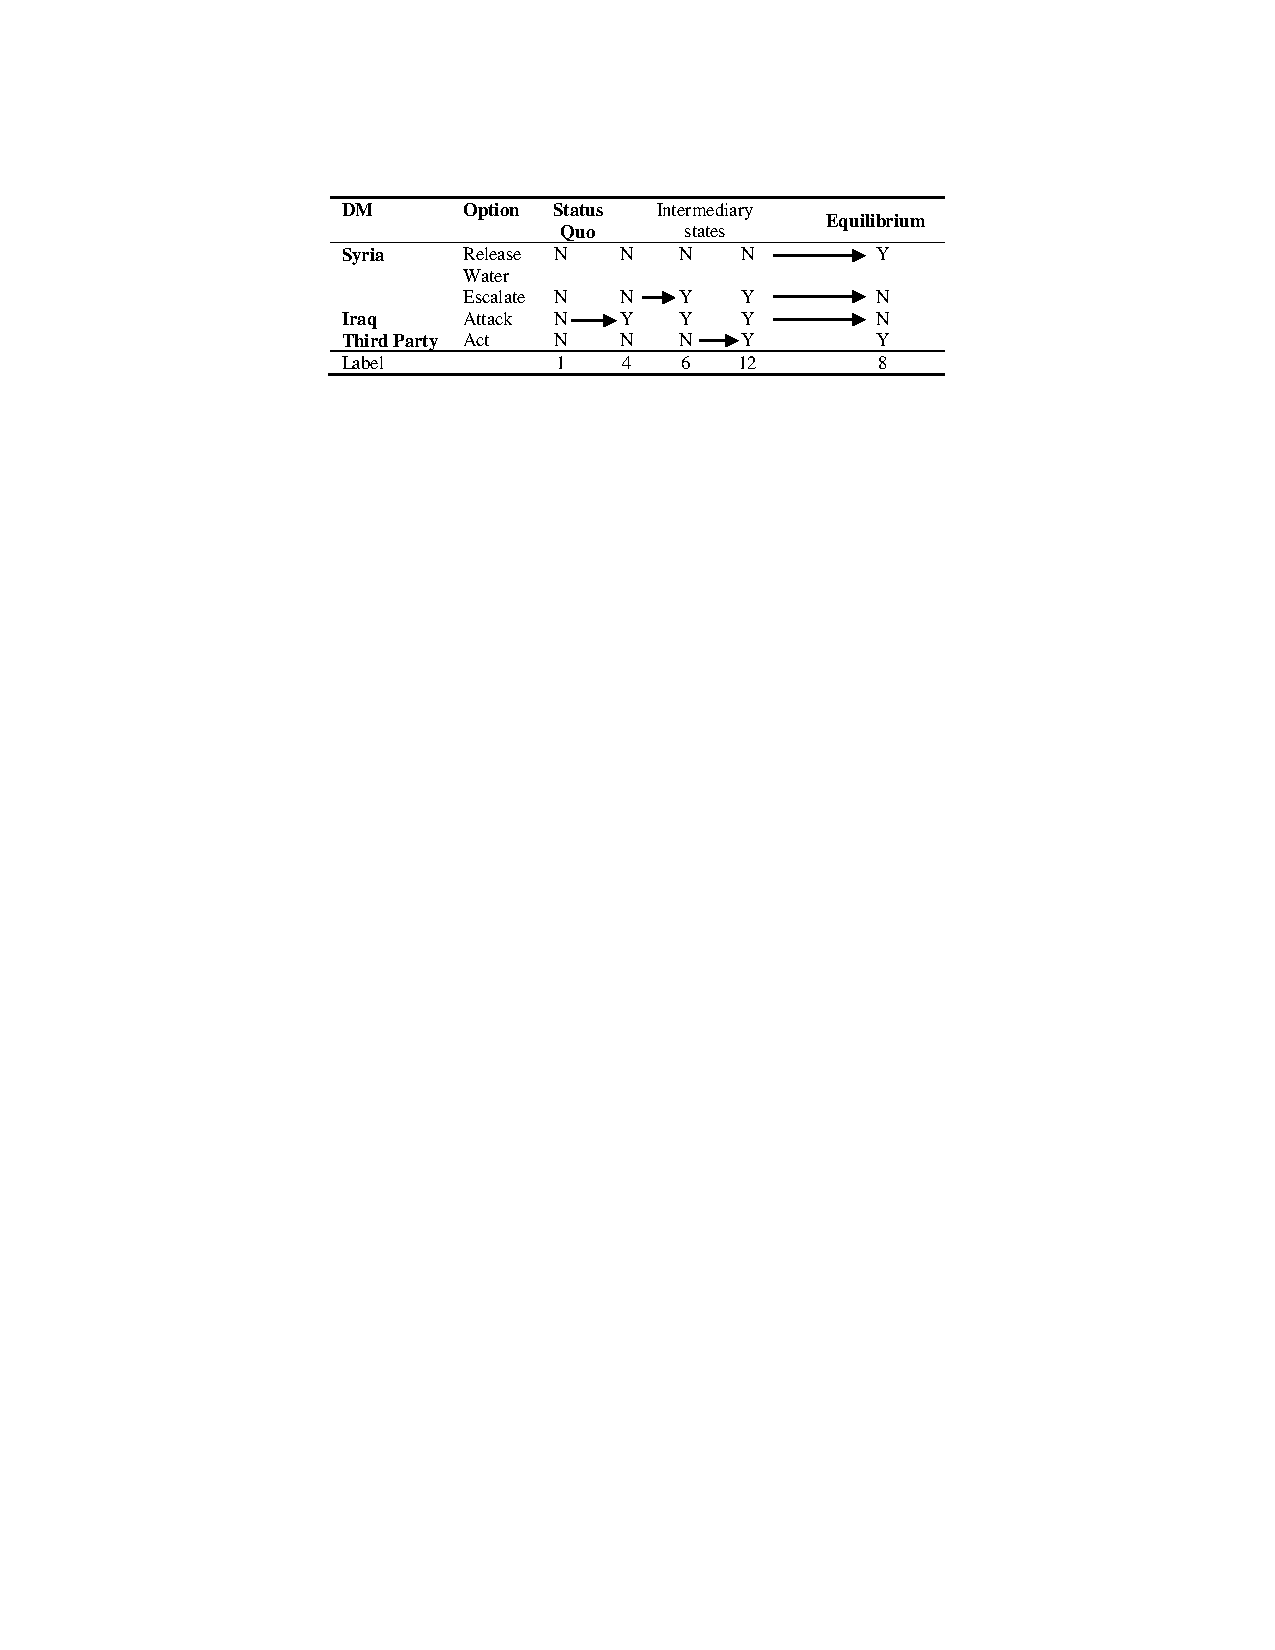
\includegraphics[scale=1]{PDF-IMG/tables/10.pdf}

\caption{Historical evolution of the 1975 conflict}

\label{tbl:t10}
\end{table}
% % % % % % % % % % % % % % % % % % % % %

\subsection{Strategic Investigation of the 1998 Controversy}
The DMs and options for the 1998 conflict are given in Table \ref{tbl:t11}. Turkey has two options: escalate the situation against Syria or carry out a full invasion. Syria has two options of stopping its support for the PKK or escalating the situation. The third party, Egypt, has a single option of acting or not.

\begin{table}[H]
\centering
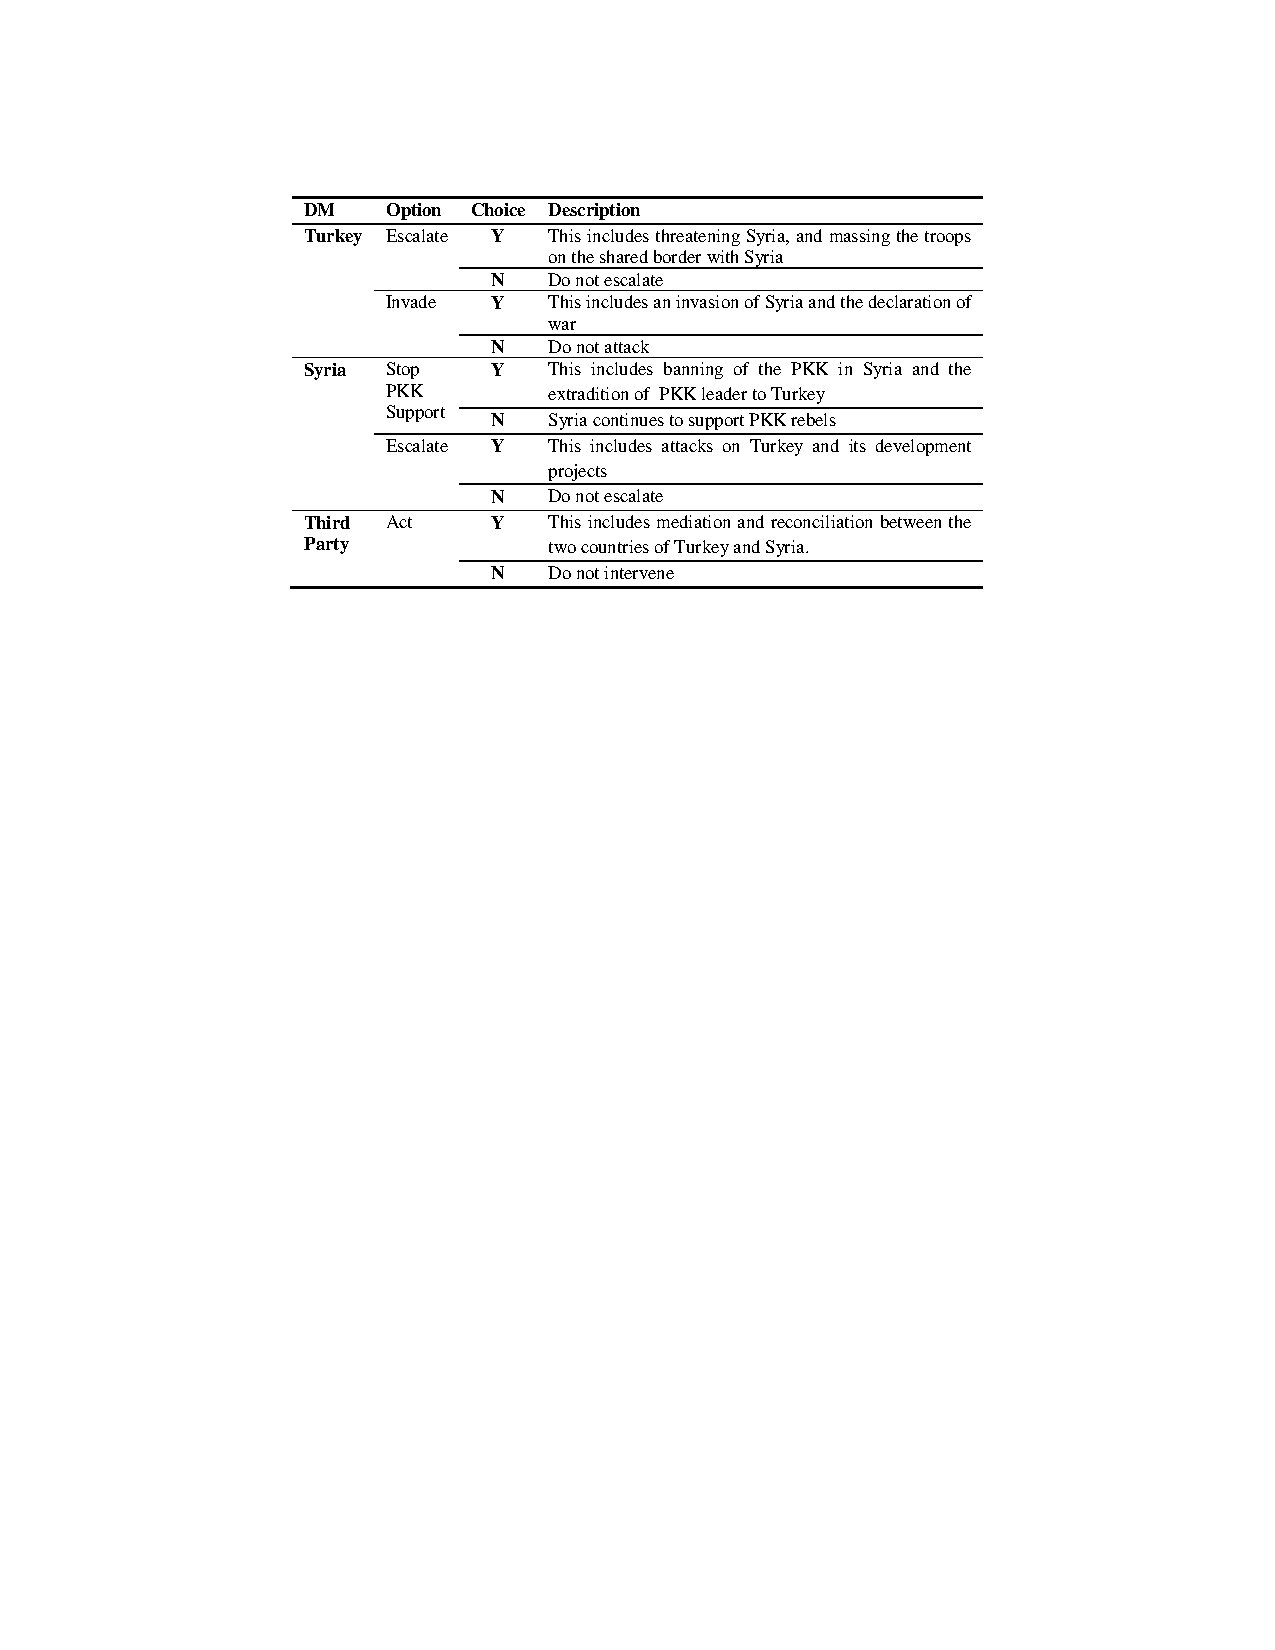
\includegraphics[scale=1]{PDF-IMG/tables/11.pdf}

\caption{DMs, options and descriptions for the 1998 conflict}

\label{tbl:t11}
\end{table}

The set of feasible states is provided in Table \ref{tbl:t12}. Note that there is one infeasible situation in which Syria can both ban PKK and escalate at the same time (mutually exclusive options). Also notice that state 9 is an indistinguishable state if Turkey decides to invade Syria, since a full scale war will occur and the game will end.  Because the third party played an Arbitrator role in this conflict, the situation in which it acts and Syria does not ban the PKK, is removed. The remaining possible states or scenarios are provided in Table \ref{tbl:t12}. Figure \ref{fig:SyTrGM} shows the Integrated Graph Model of the conflict.

\begin{table}[H]
\centering
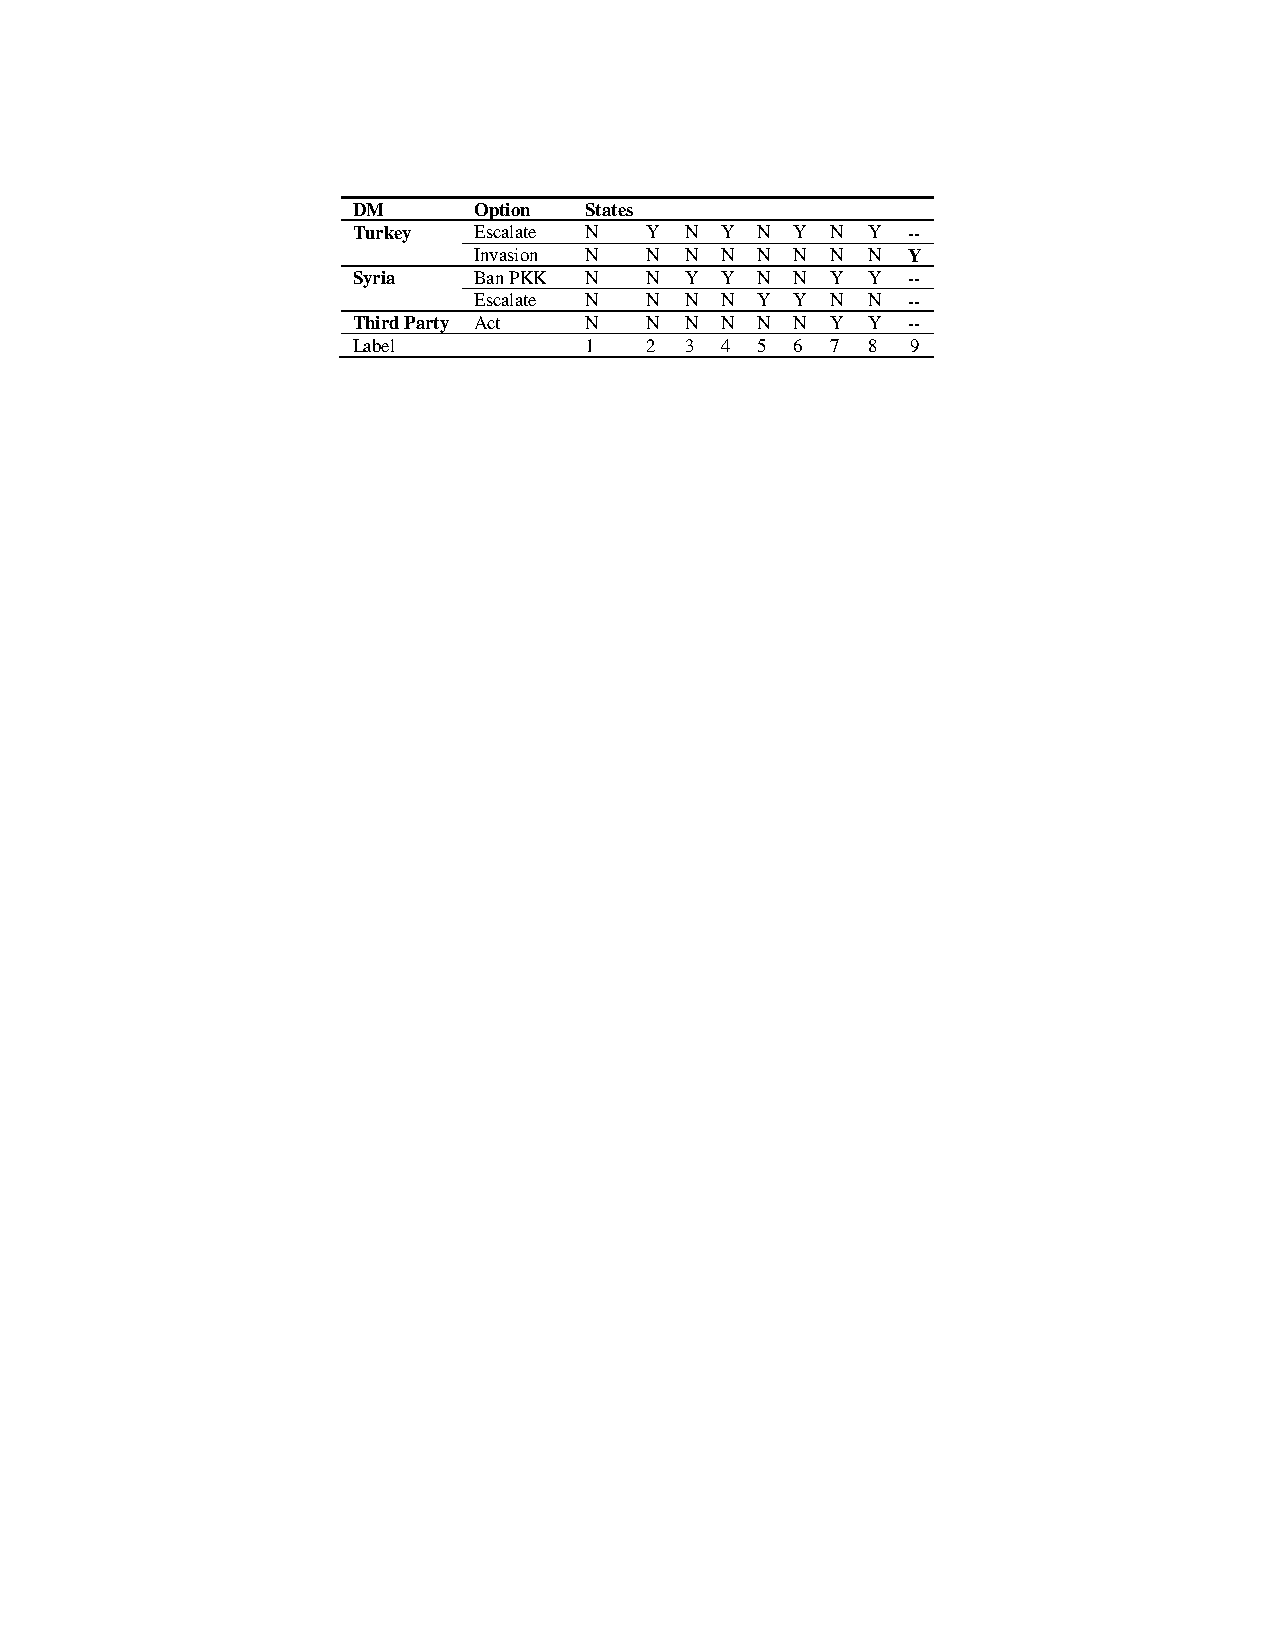
\includegraphics[scale=1]{PDF-IMG/tables/12.pdf}

\caption{DMs, options and states for the 1998 conflict with the third party}

\label{tbl:t12}
\end{table}

\begin{center}
\begin{figure}[H]
\centering
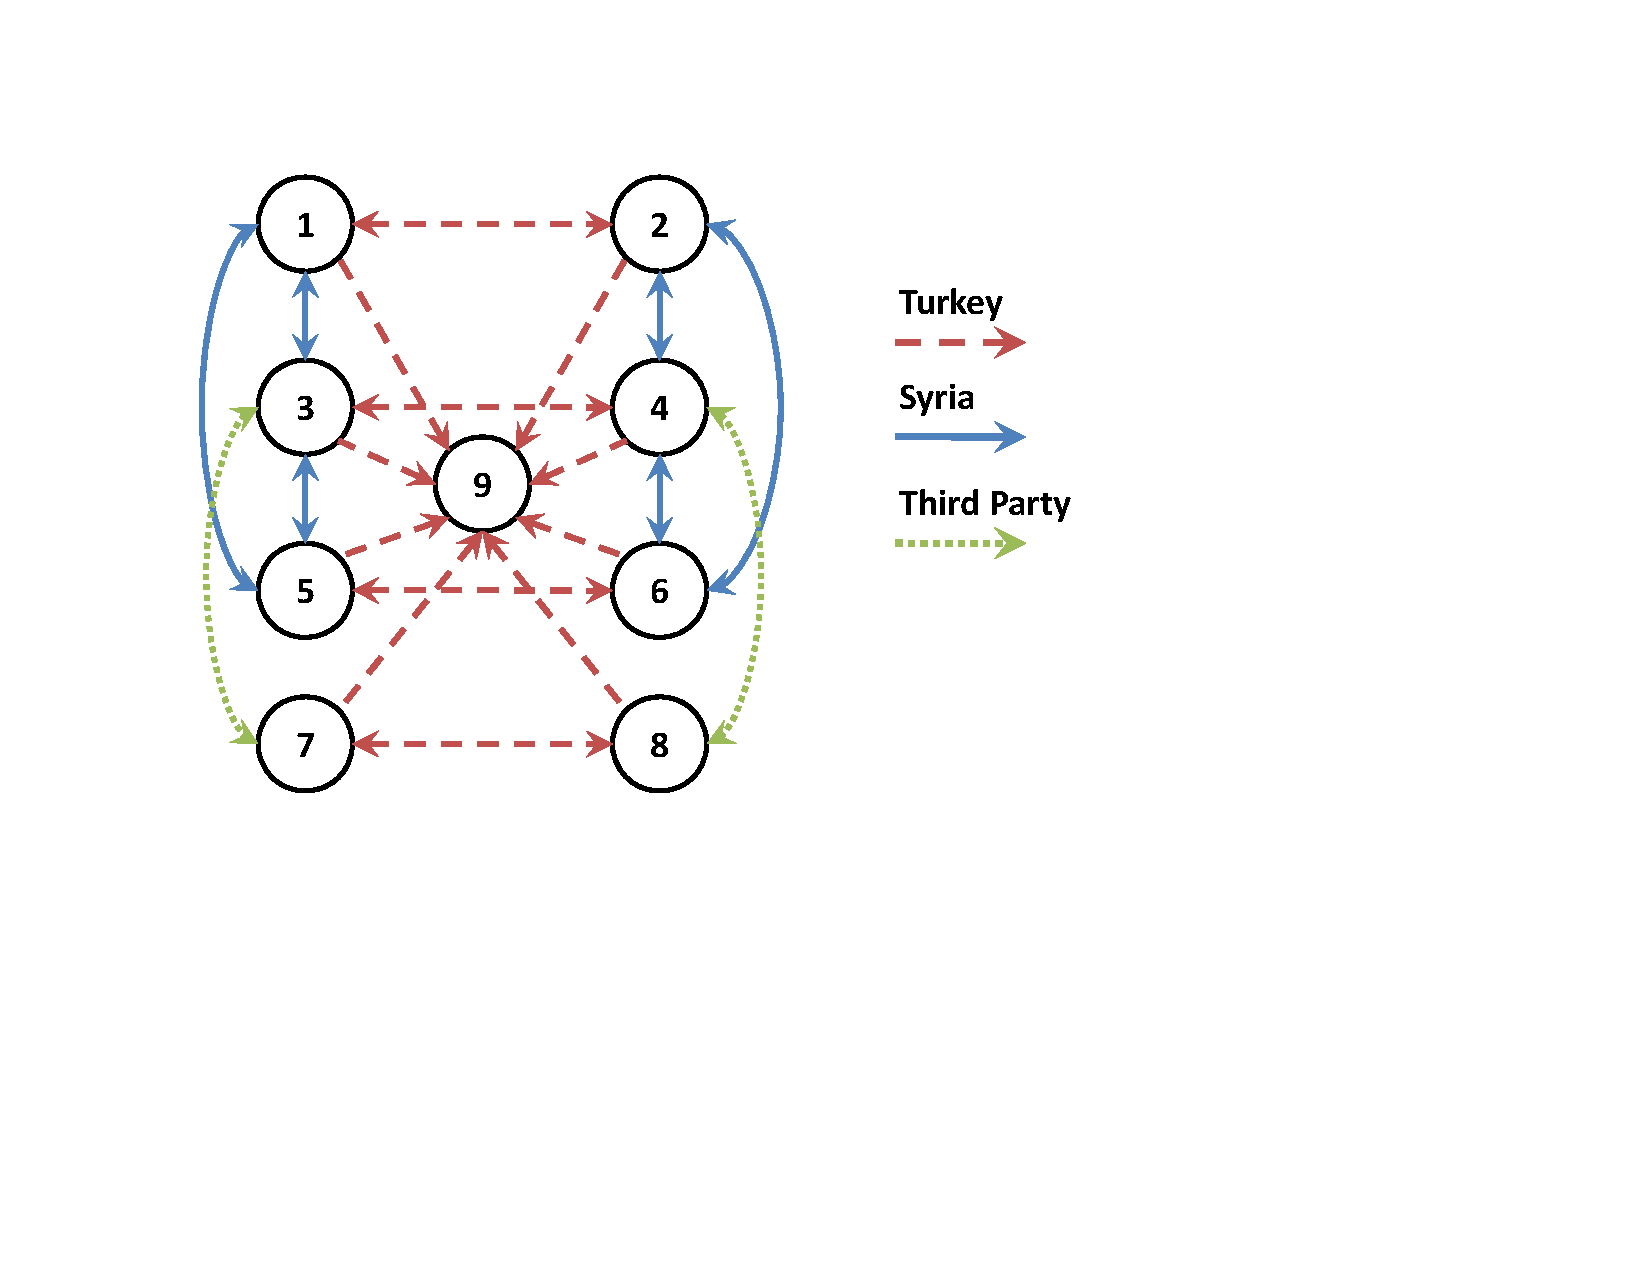
\includegraphics[scale=0.6]{PDF-IMG/SyTrEg.pdf}

\caption{Integrated Graph Model of the 1998 conflict with the third party}

\label{fig:SyTrGM}
\end{figure}
\end{center}

In this situation, the third party acts as an Arbitrator, since the party has the power to exclude some states \citep{sakamoto2005}. In this conflict, the third party, Egypt, restricted Syria's move of not banning the PKK if it intervened. Egypt brings to the table legitimacy and extensive experience gained through experience with the conflicts along the Nile basin \citep{akanda2007tigris}. Syria was united with Egypt under the United Arab Republic (UAR) before Syria declared independence from the UAR in the 1970s. UAR was mostly led by the Egyptian President, Gamal Abdel Nasser. These factors combined to give Egypt a say in Syria's politics. Table \ref{tbl:t13} presents the preference prioritization information for each DM in the 1998 conflict from most to least preferred. Table \ref{tbl:t14} presents the hierarchical preference statements for Turkey, Syria, and the third party from most to least important. Table \ref{tbl:t15} outlines the analysis results after inputting the foregoing information into GMCR II. 

\begin{table}[H]
\centering
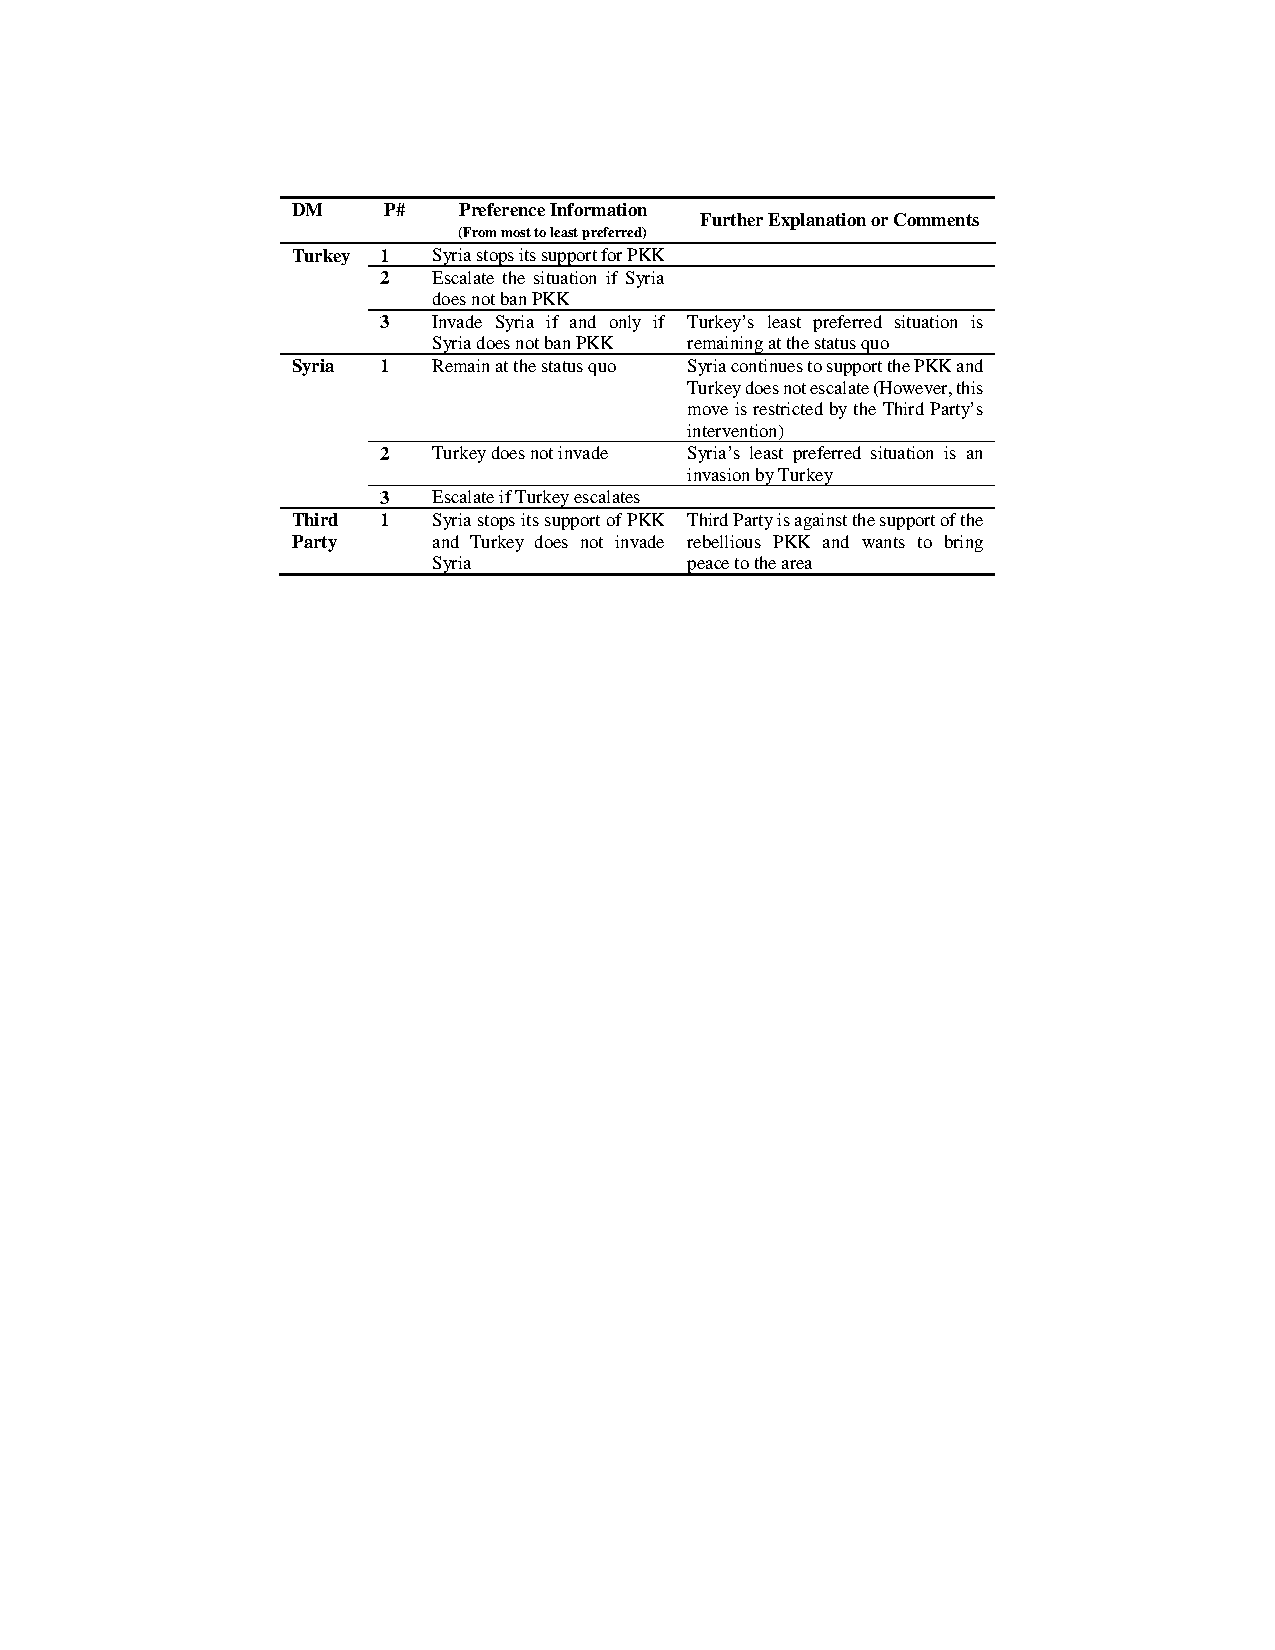
\includegraphics[scale=1]{PDF-IMG/tables/13.pdf}

\caption{Preference prioritization information for the 1998 conflict with the third party}

\label{tbl:t13}
\end{table}

\begin{table}[H]
\centering
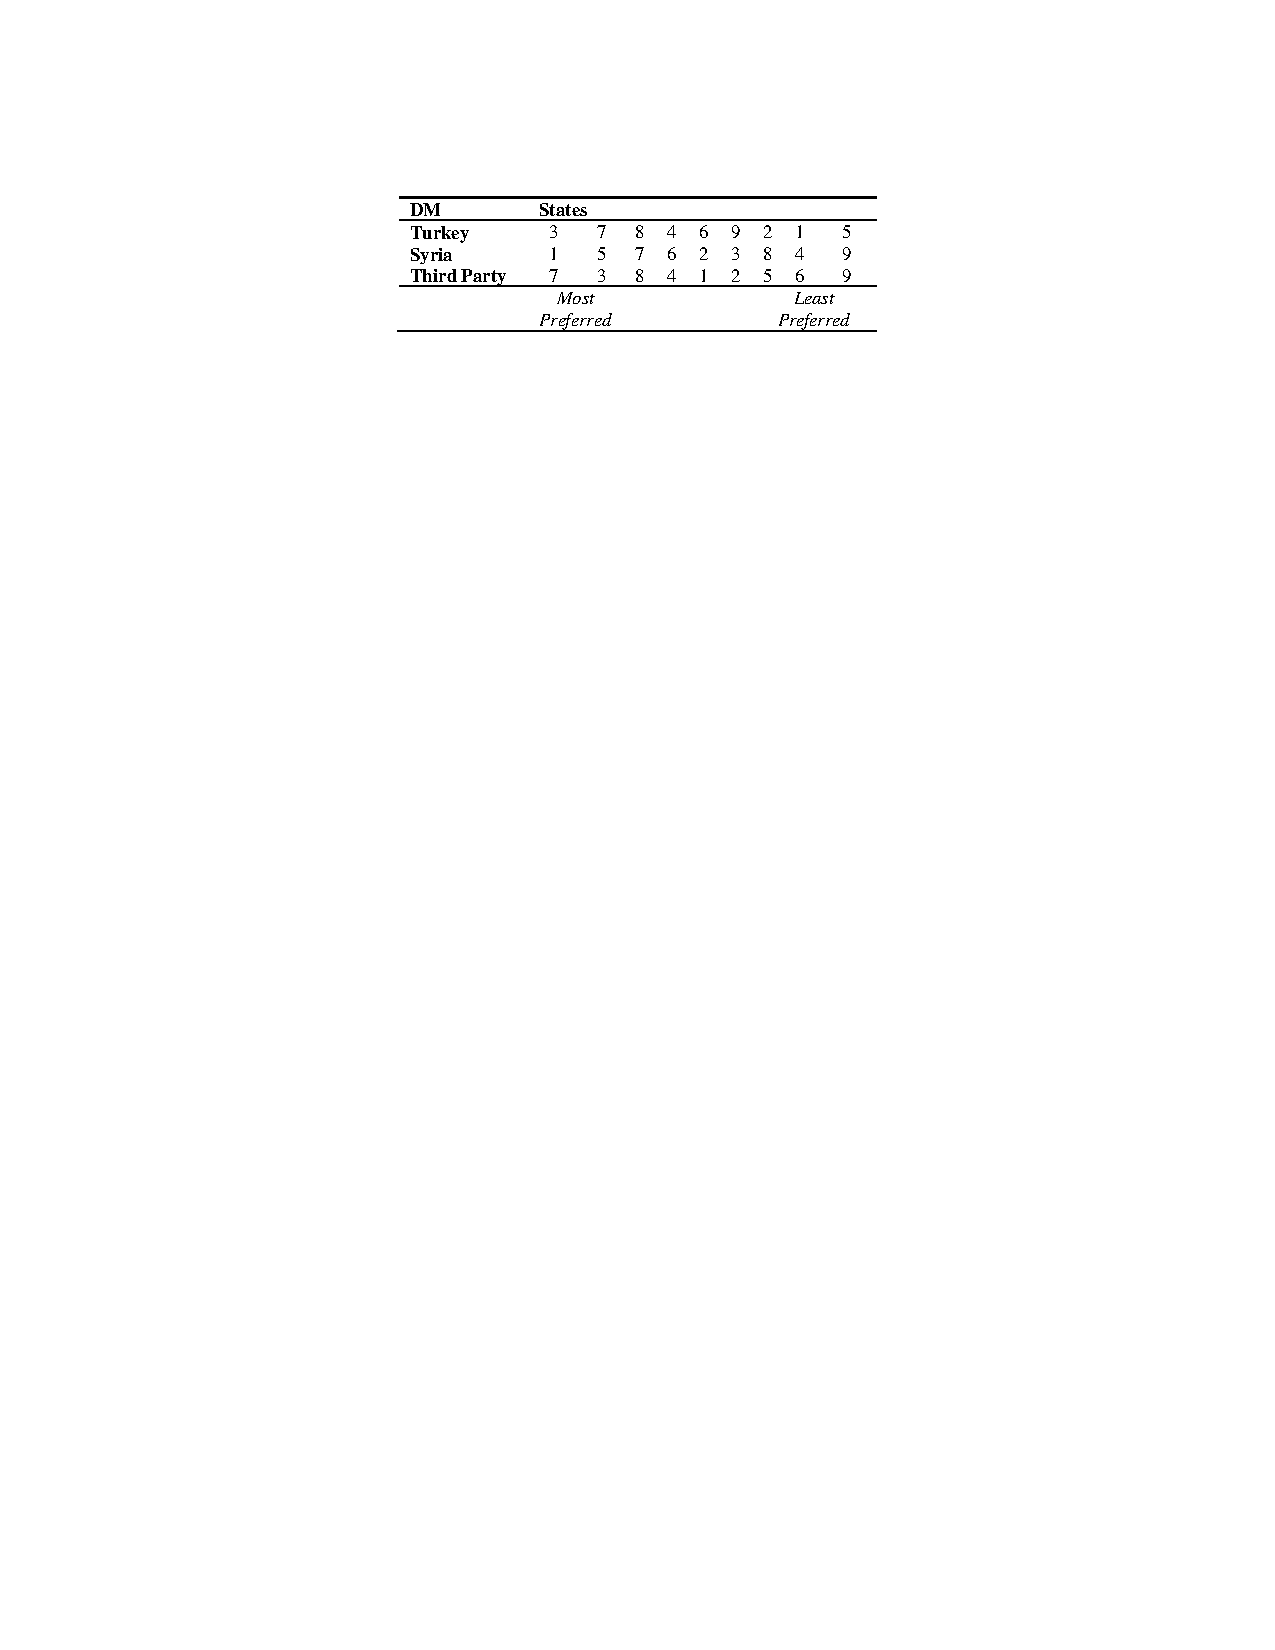
\includegraphics[scale=1]{PDF-IMG/tables/14.pdf}

\caption{Ranking of states for DMs in the 1998 conflict with the third party}

\label{tbl:t14}
\end{table}

\begin{table}[H]
\centering
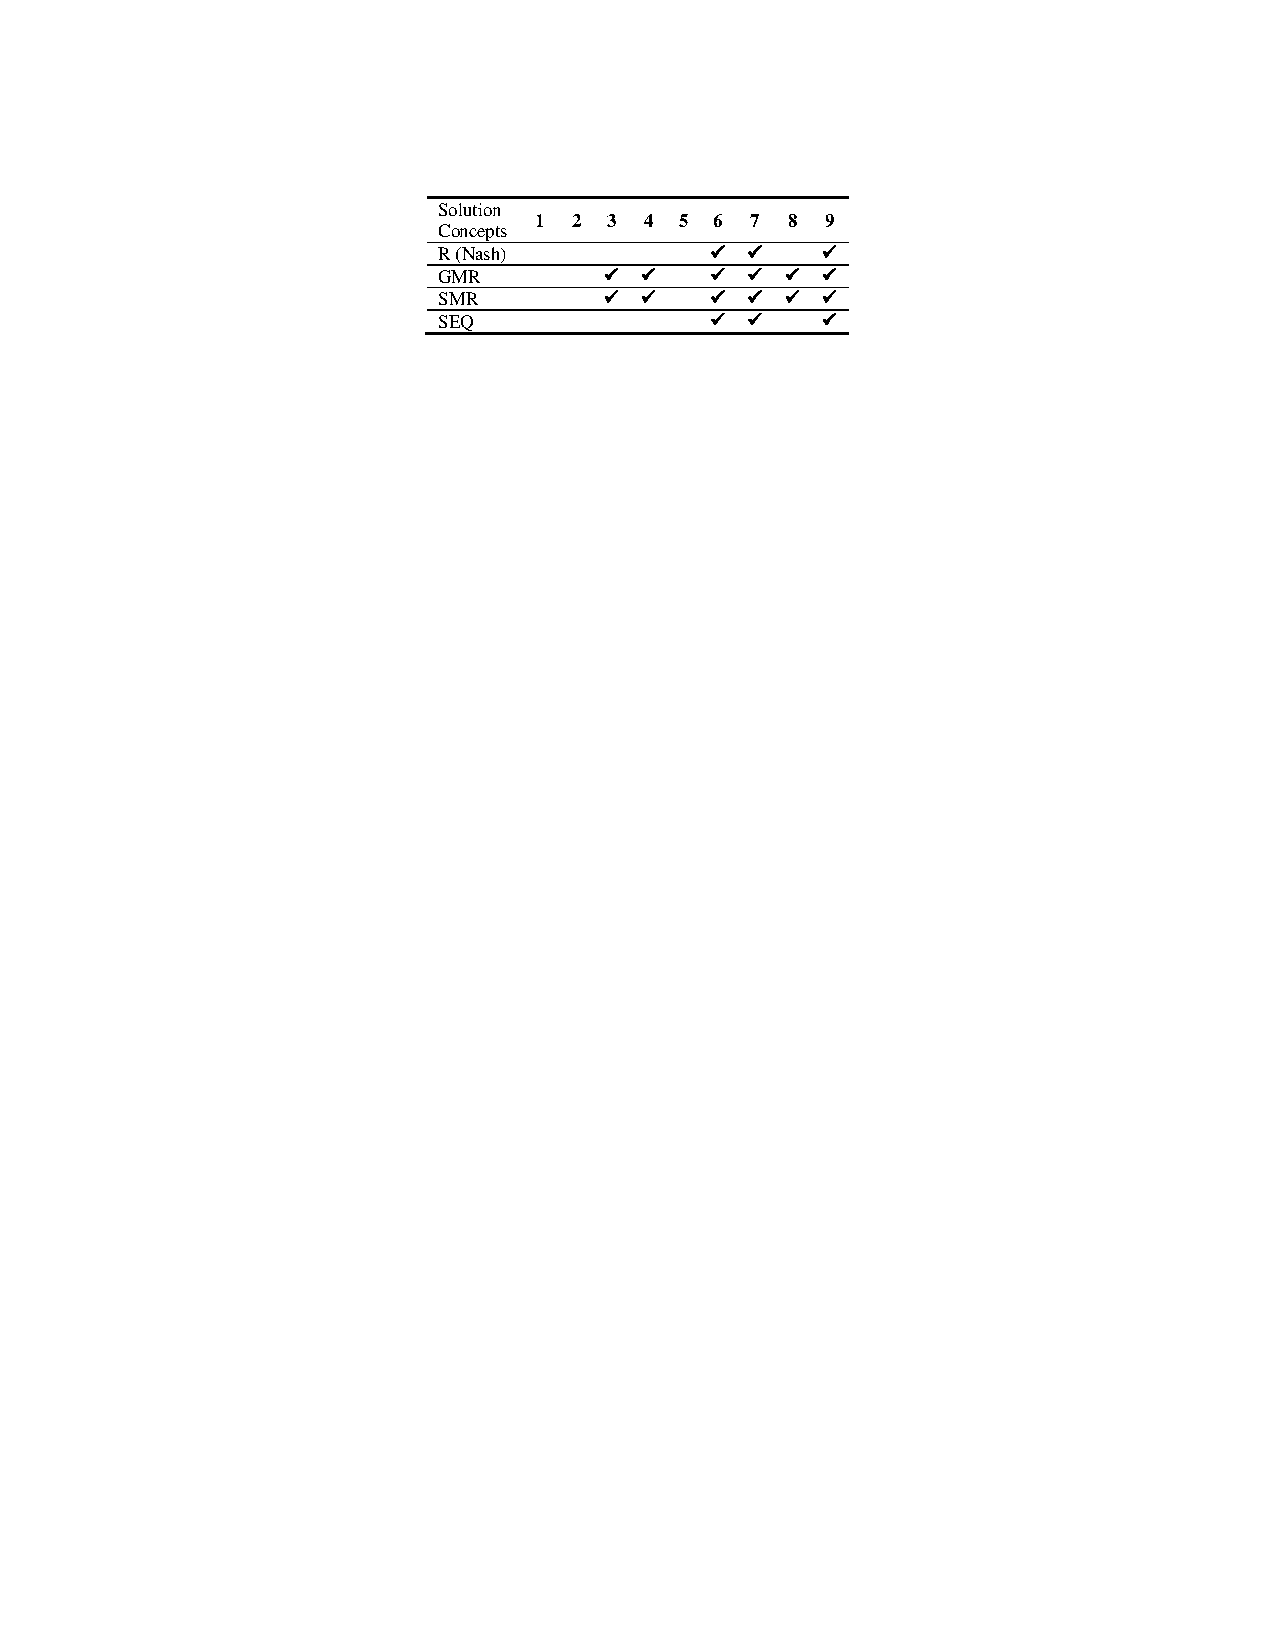
\includegraphics[scale=1]{PDF-IMG/tables/15.pdf}

\caption{Equilibrium results for the 1998 conflict with the third party}

\label{tbl:t15}
\end{table}

This conflict study shows that Turkey played a more important role than Syria and did not have to use water as a weapon. Moreover, Turkey's superior military power puts it at an advantage, which allowed it to threaten Syria with an invasion, thereby bringing the game to an end. The strongest equilibrium states are 6 and 9 (Table \ref{tbl:t15}) in which both Syria and Turkey escalate the situation and Turkey invades eventually if the third party does not act. However, with the mediation of the third party, a new equilibrium came about: state 7 in which the third party acts and Syria bans the PKK. As will be explained in the final section, Syria has been put in a Pareto-inferior situation as it had to give up other things in addition to banning the PKK.
The notion of classifying the role of the third party into Arbitrator, Coordinator, and Donor can determine, in advance, how a third party can influence and bring about a potential resolution to the conflict. Table \ref{tbl:t16} shows the actual historical evolution of the 1998 conflict. 


\begin{table}[H]
\centering
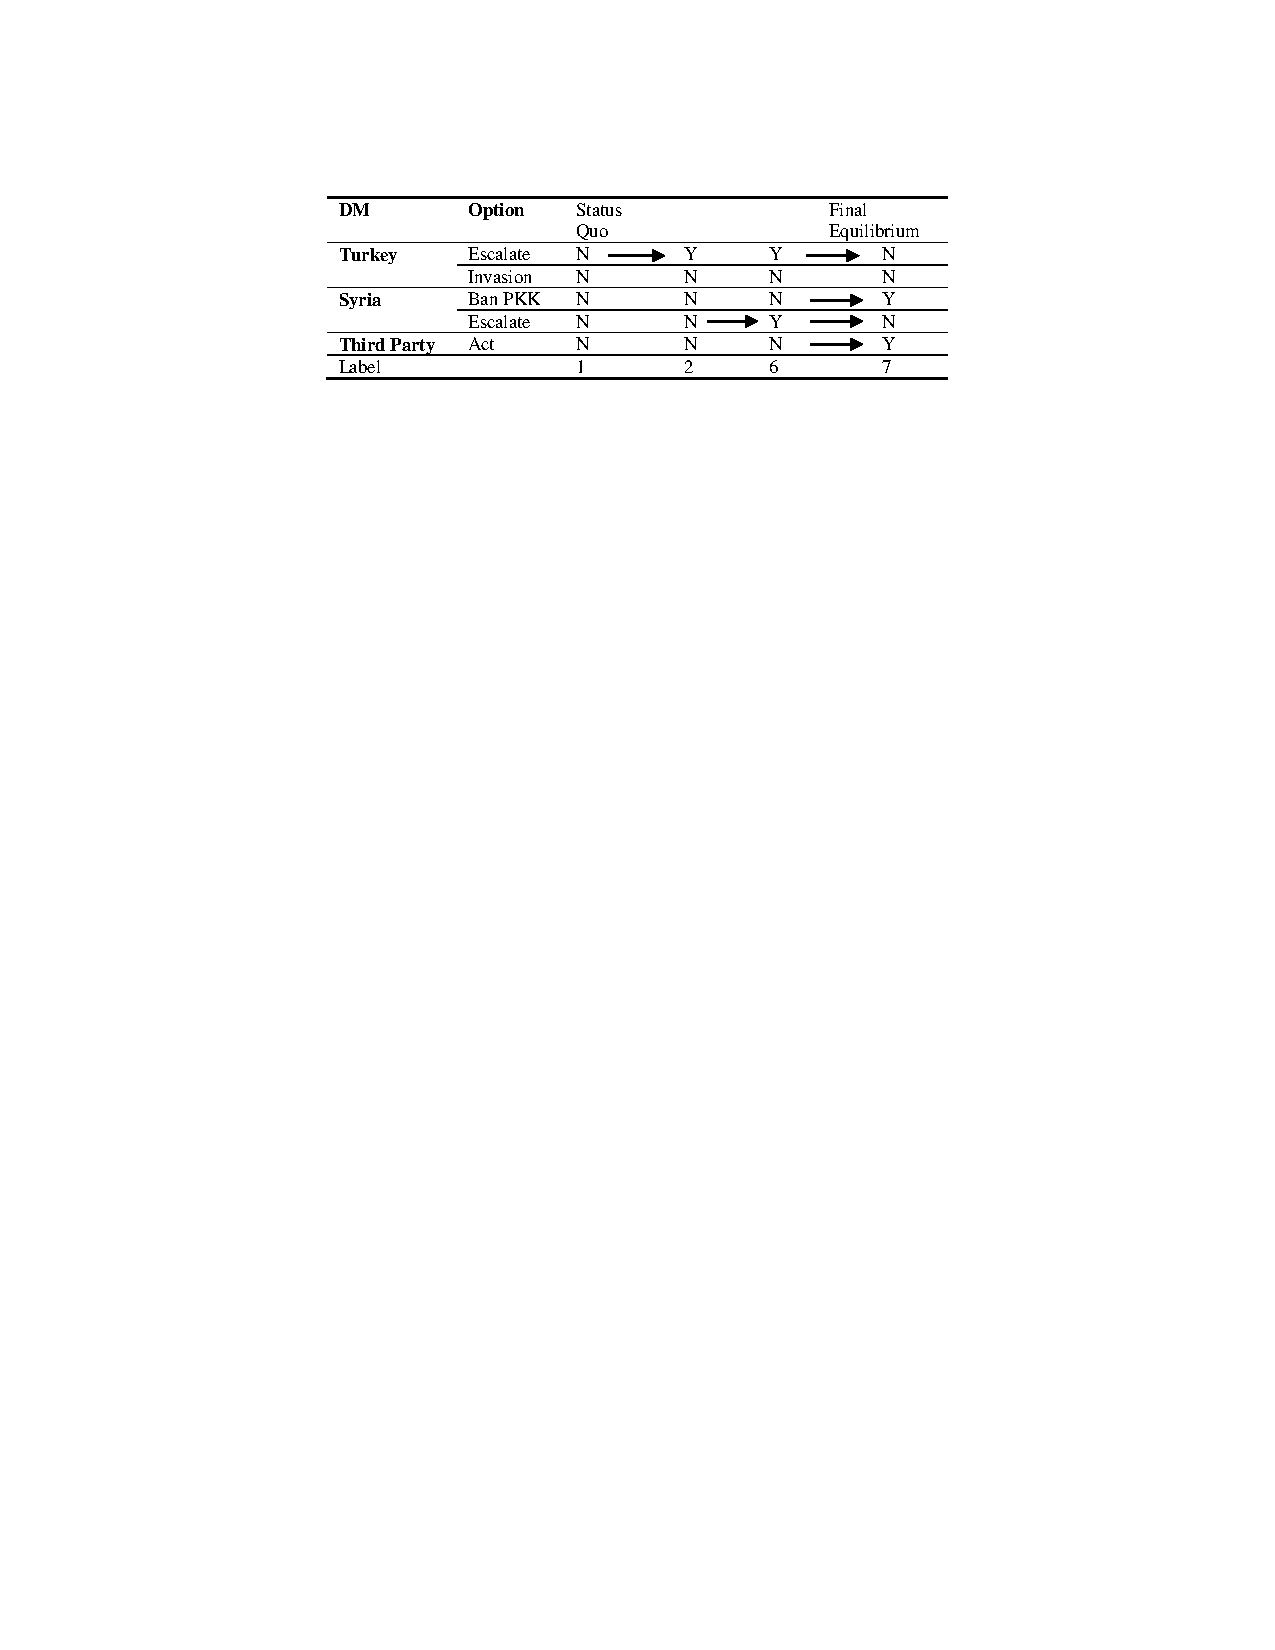
\includegraphics[scale=1]{PDF-IMG/tables/16.pdf}

\caption{Historical evolution of the 1998 conflict}

\label{tbl:t16}
\end{table}

\subsection{Fundamental Insights}
The analyses confirm similar conclusions drawn by \citet{priscoli2009managing} in their studies of Middle East water conflicts. Firstly, unilateral development of water resources without the coordination and cooperation of other countries sharing the same water recourse may create conflict. Secondly, if one riparian country holds the geographical and military power, unbiased agreements are difficult to achieve. For example, Turkey is upstream and most of the water originates in its territory. Moreover, it has the most advanced military power \citep{priscoli2009managing}, giving it the upper hand in negotiations. As a consequence, Syria ended up in a Pareto-inferior situation because it did not ban the PKK earlier in the conflict which led to the signing of the Adana Agreement. The terms of the agreement include more things Syria has to give up in addition to banning PKK. For instance, Syria accepted Turkish rule over Hatay province, a long disputed land between the two countries. Syria publicly recognized Hatay as a Turkish territory after the Adana agreement, thereby losing two of its playing cards. The third lesson that can be garnered from the case in this paper is the vital role of third party intervention in resolving conflicts.

For the analysis part, the presented conflicts, especially the conflicts in both 1990 and 1998, can be seen as a single evolving conflict. This can serve as a base for methodology development. In addition, a more in-depth analysis could be carried out by mixing various approaches to conflict analysis. For instance, one can carry out hypergame analysis and coalition analysis at the same time for the 1990 conflict.

It is clear that the conflict along the Euphrates River is indeed a complex one. Bilateral and tripartite negotiations continue with mixed success. However, no solid agreement to date has been reached. This paper forms a strong base for carrying out an in-depth analysis of the present situation and determining how the conflict could evolve and what resolution could result in the future. 

%======================================================================


\chapter{Modeling Third Party Intervention in Conflict Resolution}
%%%%%%%%%%%%%%%%%%%%%%%%%%%%%%%%%%%%%%

\section{Introduction}

In order to formally model third party intervention in conflicts, three areas will be investigated, as follows:
\begin{enumerate}
\item Inverse approach to conflict resolution: A modeling technique that will allow mediators to choose a desired outcome as equilibrium, and work backwards to achieve it.
\item Inverse status quo analysis: An extension to the previous area that determines whether the desired equilibrium is reachable from the original state.
\item Third party prediction: A tool to analyze conflicts inviting mediation and give insight as to which role a mediator should play to resolve the conflict.

\end{enumerate}

%%%%%%%%%%%%%%%%%%%%%%%%%%%

\section{Inverse Approach to GMCR}
\subsection{Overview and Objective}

The Graph Model for Conflict Resolution (GMCR) forms an ideal framework to model and analyze conflicts; however, there are challenges to its application, especially in estimating the relative preferences of DMs involved in the conflict. In order to address this problem, the inverse approach to GMCR allows the mediator to determine how a desired resolution to the conflict can arise by generating all possible preferences that achieve it.

The premise of the inverse approach is that the mediator needs a negotiation tool to influence the DMs. To be valuable, this tool should contain information about what motivates each party to undertake the options leading to the resolution desired by the mediator. Therefore, mediators can focus their resources and strategies to guide the parties toward preferences that lead to the desired resolution. This tool is not just useful to third parties; actual stakeholders can take advantage of it to influence their opponent(s).

The current GMCR framework, which forms the basis for the inverse approach, requires preference ranking information that may not be easy to obtain. The inverse approach introduces a modeling approach that requires minimal preference ranking information up front. A desired resolution, or equilibrium, is decided and a list of preference ranking information leading to the resolution is generated. Thus the inverse approach utilizes GMCR as a negotiation tool rather than a prediction tool.

The main objectives of the inverse approach to GMCR are the following:
\begin{itemize}
\item Allow a third party to determine a desired resolution and understand how to achieve it
\item Produce strategic information that will help mediators to influence the DMs involved in the conflict
\item Give a range of preference rankings that measures the robustness of the conflict resolution
\end{itemize}

In contrast, the current GMCR methodology informs the user only about the possible resolution of a conflict based on the input preferences. This approach explains how this resolution can be reached. Although this approach is motivated by the need to facilitate third party intervention, other DMs involved in the conflict can also make use of it. This approach will allow for strategic negotiation based on tactical information to achieve a desired outcome.



\subsection{Procedure and Implementation}

The main difference between the inverse approach and the standard GMCR procedure is in the order of steps. The diagram in Figure \ref{fig:procedure_or} illustrates the current procedure for applying GMCR in the real world. A modified version of the graph, shown in Figure \ref{fig:procedure_inv}, illustrates how to apply the inverse approach to GMCR. The original procedure requires the following inputs for the conflict to be analyzed: (1) decision makers (DMs), (2) options for each DM, and (3) preference rankings of the states for each DM \citep{Fang1989,fang1993}. On the other hand, the inverse approach will not require the ranking of states for all DMs. Its requirements are: (1) DMs, (2) options for each DM, (3) desired equilibrium, and (4) stability definition. The result will be a list of possible state rankings that will make the desired resolution stable under the selected stability definition.

\begin{center}
\begin{figure}[H]
\centering
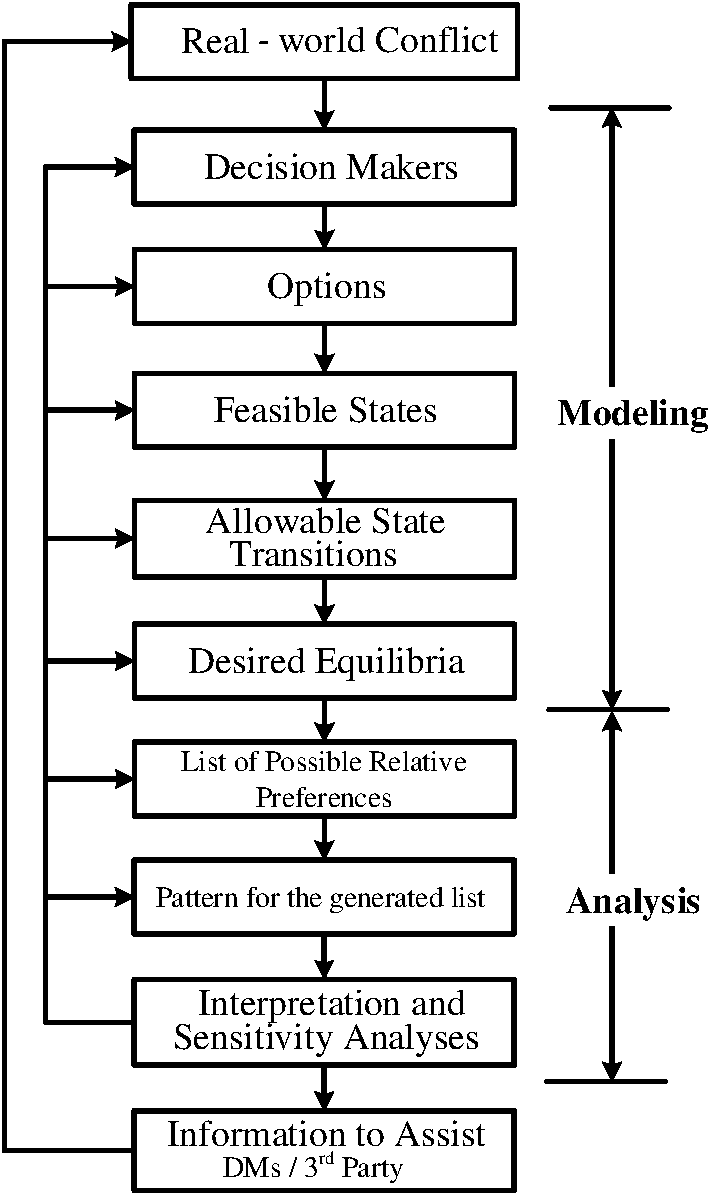
\includegraphics[scale=0.55]{PDF-IMG/GMCR_inv.pdf}

\caption{The inverse approach to GMCR procedure in a real world conflict (modified from \citet{fang1993})}

\label{fig:procedure_inv}
\end{figure}
\end{center}

In order to formally define the \textit{inverse approach to GMCR}, we need to furnish some definitions and notation. 

\begin{definition}
\rm

Let $N=\{1,2,\dots,n\}$ represent the set of DMs and $S=\{s_1, s_2, ..., s_m\}$ represent the set of feasible states in a graph model. The ordinal payoff vector of DM $i$, denoted by $P_i$, is
$$p^i=P_i=(p_1^i,p_2^i, \dots ,p_m^i ) , \quad P_i \in \mathbb{R}^m  $$

\end{definition}

\noindent If $s_a,s_b \in S$, then DM $i$ prefers $s_a$ to $s_b$ or is indifferent ($s_a \succsim_i s_b$) \emph{iff} $p_a^i \geq p_b^i$. An equivalent notation is $$P_i(s_j)=p_j^i$$ so that $s_a\succsim_i s_b$ \emph{iff} $P_i(s_a)\geq P_i(s_b)$

For example, if $P_i=(5,0,6,2,6)$ then the ordinal payoff value for DM $i$ for state 1 is equal to 5. Thus, $P_i(s_1)=5,P_i(s_2)=0,P_i(s_3)=6,P_i(s_4)=2,$ and $P_i(s_5)=6$. Because preferences are assumed to be transitive, the payoff vector can be translated into a preference profile. A preference ranking for DM $i$ is a list of feasible states ordered from most to least preferred for DM $i$. %Equally preferred states are marked with a bar or a parenthesis in the preference ranking.
In the previous example, the preference ranking for DM $i$ would be $PR_i=s_3 \sim s_5 \succ s_1 \succ s_4 \succ s_2$.

Note that the same preference ranking can be represented by many different ordinal payoff vectors. Two such ordinal payoff vectors are called equivalent.

\begin{comment}

\begin{definition}
\rm

Let $N=\{1,2,\dots,n\}$ represent the set of DMs, $S=\{s_1, s_2, \dots, s_m\}$ represent the set of feasible states in a graph model. If $s_a\succsim s_b \succsim \dots \succsim s_z$, then $PR_i=\{s_a, s_b, \dots, s_z\} $ is a preference ranking.

%and $P_i=(p_1^i,p_2^i, \dots ,p_m^i ) , \quad P_i \in \mathbb{R}^m  $ be the ordinal payoff vector of DM $i$. The preference profile for DM $i$ denoted by $PP_i$, is given by:

%where $a,b,\dots ,z \in \mathbb{N}=\{1,2,\dots ,m\} $ and $P_i(s_a)\succsim P_i(s_b)\succsim \dots \succsim P_i(s_z)$
\end{definition}

\end{comment}


\begin{definition}
\rm
If $p^i \in \mathbb{R}^m$ is a preference vector for DM $i \in N$, then $(p^1,p^2,\dots ,p^n) \in \mathbb{R}^{mn}$ is a preference profile.

\end{definition}


The inverse approach will be defined using both preference vectors and preference profiles. In the graph model, analysis means finding all equilibria given a preference profile. In the inverse approach, the problem is to find all preference profiles under which a given state is an equilibrium under a selected stability definition.  After the introduction of preference profiles, a graph model can be denoted $G=\langle N,S,P\rangle$ where $N$ is the list of DMs $N=\{1,\dots ,n\}$, $S$ is the set of feasible states $S=\{1,\dots ,m\}$, and $P$ is the preference profile $P \in \mathbb{R}^{mn}$.

The \emph{inverse problem} for a desired equilibrium state $s_E \in S$ is to find all $p \in \mathbb{R}^{mn}$ such that state $s_E$ is stable for all DMs if the preference profile is $p$.


\noindent \textbf{Inverse Nash problem for $s_E$:} Find $p \in \mathbb{R}^{mn}$ such that $s_E \in Nash(G)$ where $G=\langle N,S,P\rangle $

\noindent \textbf{Inverse SEQ problem for $s_E$:} Find $p \in \mathbb{R}^{mn}$ such that $s_E \in SEQ(G)$ where $G=\langle N,S,P\rangle $

\noindent \textbf{Inverse GMR problem for $s_E$:} Find $p \in \mathbb{R}^{mn}$ such that $s_E \in GMR(G)$ where $G=\langle N,S,P\rangle $

\noindent \textbf{Inverse SMR problem for $s_E$:} Find $p \in \mathbb{R}^{mn}$ such that $s_E \in SMR(G)$ where $G=\langle N,S,P\rangle $

A more formal definition according to each solution concept will follow.


\subsection{Algorithms}

In order to implement the inverse approach, two approaches were investigated. The first one was the brute-force method. As the name suggests, this method tests each possible preference profile for each DM against the desired equilibrium. Since the number of possible preference rankings is fairly large, a decision support system was designed to test the concept. The number of iterations required for a model, assuming strict ordinal preferences, is given by $(m!)^{n}$ where $m$ is the number of feasible states and $n$ is the number of DMs.  If the combination of preference vectors for all DMs (i.e. preference profile) achieves the desired equilibrium, it will be saved into a list. The second algorithm was designed after observing the pattern produced by the brute-force method. It was clear that results followed certain rules which can be defined more formally, as outlined in the following subsections. %The pseudo-codes for both algorithms will be given in the decision support system section below.%



\subsection{Inverse Nash Equilibrium}
\begin{definition}
\rm
\label{def:nash_inv1}
State $s_E$ is a Nash equilibrium $iff$ $p_i(s)\leq p_i(s_E)$ for all $i \in N$ and all $s \in R_i(s_E)$


%all states $s_(m-E) \in R^{+}_{n}(s)$ for all $n \in N$ must satisfy  $q <_{N} s$ in all $P_{N}$
\end{definition}

%\begin{theorem}
%\rm
%\label{thm:nash_inv2}

%If all states $q \in R^{+}_{n}(s)$ satisfy $q <_{n} s$ for all $n \in N$, then state $s$ is Nash stable.
%\end{theorem}

Thus, the inverse approach should produce all preference profiles that make the desired state $s_E$ a Nash equilibrium. For illustration, the inverse approach list according to preference profiles (or payoff vectors), denoted by $IPV(s_E)$, is shown in fig \ref{fig:IPVil}. Note that each of the $T$ rows is a preference profile which is a combination of preference vectors that will make state $s_E$ stable for all DMs. The possible number of profiles is denoted by $T$. %Similarly, the inverse approach list according to preference rankings, denoted by $IPR(s_E)$, is shown.

\noindent Note that $^hp_j^i$ is player $i$'s ordinal payoff for state $j$ in profile $h$.

\begin{center}
\begin{figure}[H]
\centering


$IPV(s_E)= \begin{Bmatrix}
[^1p_1^1,^1p_2^1, \dots ,^1p_m^1 ] & [^1p_1^2,^1p_2^2, \dots ,^1p_m^2 ] & \dots & [^1p_1^n,^1p_2^n, \dots ,^1p_m^n ] \\ 
[^2p_1^1,^2p_2^1, \dots ,^2p_m^1 ] & [^2p_1^2,^2p_2^2, \dots ,^2p_m^2 ] & \dots & [^2p_1^n,^2p_2^n, \dots ,^2p_m^n ] \\ 
\vdots  & \vdots  & \ddots  & \vdots \\ 
[^Tp_1^1,^Tp_2^1, \dots ,^Tp_m^1 ] & [^Tp_1^2,^Tp_2^2, \dots ,^Tp_m^2 ] & \dots & [^Tp_1^n,^Tp_2^n, \dots ,^Tp_m^n ]
\end{Bmatrix} $



\caption{Representation of the inverse preference profiles list for state $s_E$}

\label{fig:IPVil}
\end{figure}
\end{center}

\begin{definition}
\rm
A \emph{Nash $IPV(s_E)$} is a list of preference profiles, $p \in \mathbb{R}^{mn}$, where in each profile, for all $i \in N$, all $q \in R^{+}_{i}(s_E)$ satisfies $P_i(q)\leq P_i(s_E)$.
\end{definition}

\subsection{Inverse SEQ Equilibrium}

\begin{definition}
\rm
\label{def:seq_inv}
An \emph{SEQ $IPV(s_E)$} is a list of preference profiles, $p \in \mathbb{R}^{mn}$, such that for each state $q \in R^{+}_{i}(s_E)$ in the preference profile, there exists at least one state $k\in R^{+}_{N-i}(q)$ satisfying $P_i(k)\leq P_i(s_E)$ for all %$q \in  R^{+}_{i}(s_E)$ and all 
$i \in N$ 
\end{definition}

In other words, the combination of payoff vectors must ensure that for each UI a DM can take, there exists at least one sanction that will put the original player in a less preferred state. Please note that the notation $N-i$ means all DMs other than $i$.

%\begin{definition}
%\rm
%An \emph{SEQ IPR(S)} is a combination of $P_{N}$ such that, for all UI states $s_{1} \in R^{+}_{i}(s)$, there exist at least one $q \in R_{N-i}^{+}(s_{1})<_{i} s$ for all $i \in N$
%\end{definition}


\subsection{Inverse GMR Equilibrium}

\begin{definition}
\label{def:gmr_inv}
\rm
A \emph{GMR $IPV(s_E)$} is a list of preference profiles, $p \in \mathbb{R}^{mn}$, such that for each state $q \in R^{+}_{i}(s_E)$ in the preference profile, there exists at least one state $k\in R_{N-i}(q)$ satisfying $P_i(k)\leq P_i(s_E)$ for all %$q \in  R^{+}_{i}(s_E)$ and all 
$i \in N$ 
\end{definition}

%\begin{definition}
%\rm
%\label{def:gmr_inv}
%A \emph{GMR IPR(S)} is a combination of $P_{N}$ such that, for all UI states $s_{1} \in R^{+}_{i}(s)$, there exist at least one $q \in R_{N-i}(s_{1})<_{i} s$ for all $i \in N$
%\end{definition}

\subsection{Inverse SMR Equilibrium}

\begin{definition}
\label{def:smr_inv}
\rm
An \emph{SMR $IPV(s_E)$} is a list of preference profiles, $p \in \mathbb{R}^{mn}$, such that for each state $q \in R^{+}_{i}(s_E)$ in the preference profile, there exists at least one state $k\in R_{N-i}(q)$ satisfying $P_i(k)\leq P_i(s_E)$ and all $h \in R_{i}(k)$ satisfy $P_i(h)\leq P_i(s_E)$ for all %$q \in  R^{+}_{i}(s_E)$ and all %
$i \in N$ 
\end{definition}

%\begin{definition}
%\label{def:smr_inv}
%\rm
%An \emph{SMR IPR(S)} is a combination of $P_{N}$ such that, for all UI states $s_{1} \in R^{+}_{i}(s)$, there exist at least one $q \in R_{N-i}(s_{1})<_{i} s$ for all $i \in N$ and all $k \in R_{i}(q)<_{i} s$ for all $i \in N$
%\end{definition}



\subsection{Example}

In order to illustrate the inverse approach, the example in section \ref{sec:example1} will now be analyzed using the inverse approach. A desired state is chosen to be the resolution of the conflict. The desired state is state 2, in which both Syria and Iraq stop escalating and water is released to Iraq (Table \ref{tbl:t2}). Because the mediator is aiming to influence Syria, the preference ranking for Iraq will be considered fixed (Table \ref{tbl:t5}). The objective is to assist the third party at influencing Syria and choosing the best strategy to achieve the desired resolution. For this example, the decision support system was used to execute the inverse approach. The findings indicate that 240 possible preference profiles can achieve the desired resolution. After analyzing these results, two meaningful patterns were identified that lead the conflict to the desired equilibrium:
\begin{itemize}
\item If Syria has state 2 as the most preferred state (Nash Stability)
\item If and only if Syria prefers states 4, 5, or 6 to state 2 (Sequential Stability)
\end{itemize}

In other words, state 2 will be the resolution to the conflict if and only if (1) Syria prefers not to escalate or (2) being attacked by Iraq is less preferred for Syria. Having this strategic information could be vital to the mediators as they focus their efforts on influencing Syria to change its preference rankings. Consequently, the final outcome of the conflict will change.

%%%%%%%%%%%%%%%%%%%%%%%%%%%


%%%%%%%%%%%%%%%%%%%%%%%%%%%%%

\section{Decision Support System}

The introduction of the inverse approach makes the need for a decision support system obvious. Solving problems by hand is possible but tiresome, time consuming, and error-prone. First, a code to test each preference profile was developed. This is called the Brute-Force method
The matrix approach to GMCR allows for faster processing \citep{xu2007matrix,xu2009}. The last decision support system, GMCR II, was developed by Xiaoyoung (John) Peng back in 1999 \citep{peng1999decision}. Until recently, no significant update was made to the decision support system, even though, the program had issues that sometimes caused it to crash or display error messages.
A project to combine both the logical and matrix approaches into a more robust and flexible decision support system was initiated by Oskar Petersons and Rami Kinsara under the supervision of Prof. Keith Hipel and Prof. D. Marc Kilgour. The objective of this system is to overcome the limitations in the previous version and also add new extensions and capabilities that it did not support. A main objective of the new system is to include the inverse approach methodology. An important feature of the software is the ability to narrate the output results. More extensions and features are planned.

%%%%%%%%%%%%%%%%%%%%%%%%%%%%%



%======================================================================
\chapter{Future Work and Timeline}
In addition to the methodologies presented in this proposal, several important topics are outlined in the following sections and will be investigated. These topics fall within third party modeling in conflict resolution.
\section{Third Party Strategy Recommendations}
Various third party roles and strategies are investigated and presented in Chapter 2 of this proposal. A methodology is needed to determine the best role and strategy that a mediator should undertake in any particular conflict situation. The motivation to introduce such a methodology is to operationalize the notion of third party intervention.

\section{Enhance the Inverse Approach Methodology}
Although basic features of the inverse approach are outlined in this proposal, further enhancements are planned to extend the capability and usefulness of the methodology. One area being studied is the development of a cost and payoff extension to the inverse approach to GMCR. This feature will allow for narrowing down the list of possible profiles and will allow for more relevant and meaningful results.

\section{Inverse Status Quo Analysis}
An inverse approach to determine the required starting points in order to attain desired equilibria will be investigated. This will be achieved by tracking the evolution of the conflict backward from a desired equilibrium to the status quo states.


\section{In-Depth Sensitivity Analysis}
As mentioned earlier, with the introduction of the inverse approach, a more in-depth model for sensitivity analysis that determines the robustness of any equilibrium by outlining the range of preference profiles in a conflict will be put forward. 

\section{Decision Support System}
Work has already started on a new decision support system using both the logical and matrix approaches for GMCR calculations. The new decision support system has the capability to perform basic inverse approach calculations using the definitions presented herein. In addition, the software will have the capability to perform regular and inverse status quo analysis. It should be noted that extensions made to the graph model for conflict resolution can be easily embedded into the new decision support system.

\section{Application to Real World Conflicts}
In order to better understand and appreciate the insights of the proposed methodologies, real world examples will be analyzed and investigated. The intention is to apply the methodologies to different conflict types, including political, environmental, and business conflicts.
\section{Timeline}
The research goals and approximate completion dates are summarized and outlined in Table \ref{tbl:milestones} below.
\begin{table}[H]
\centering
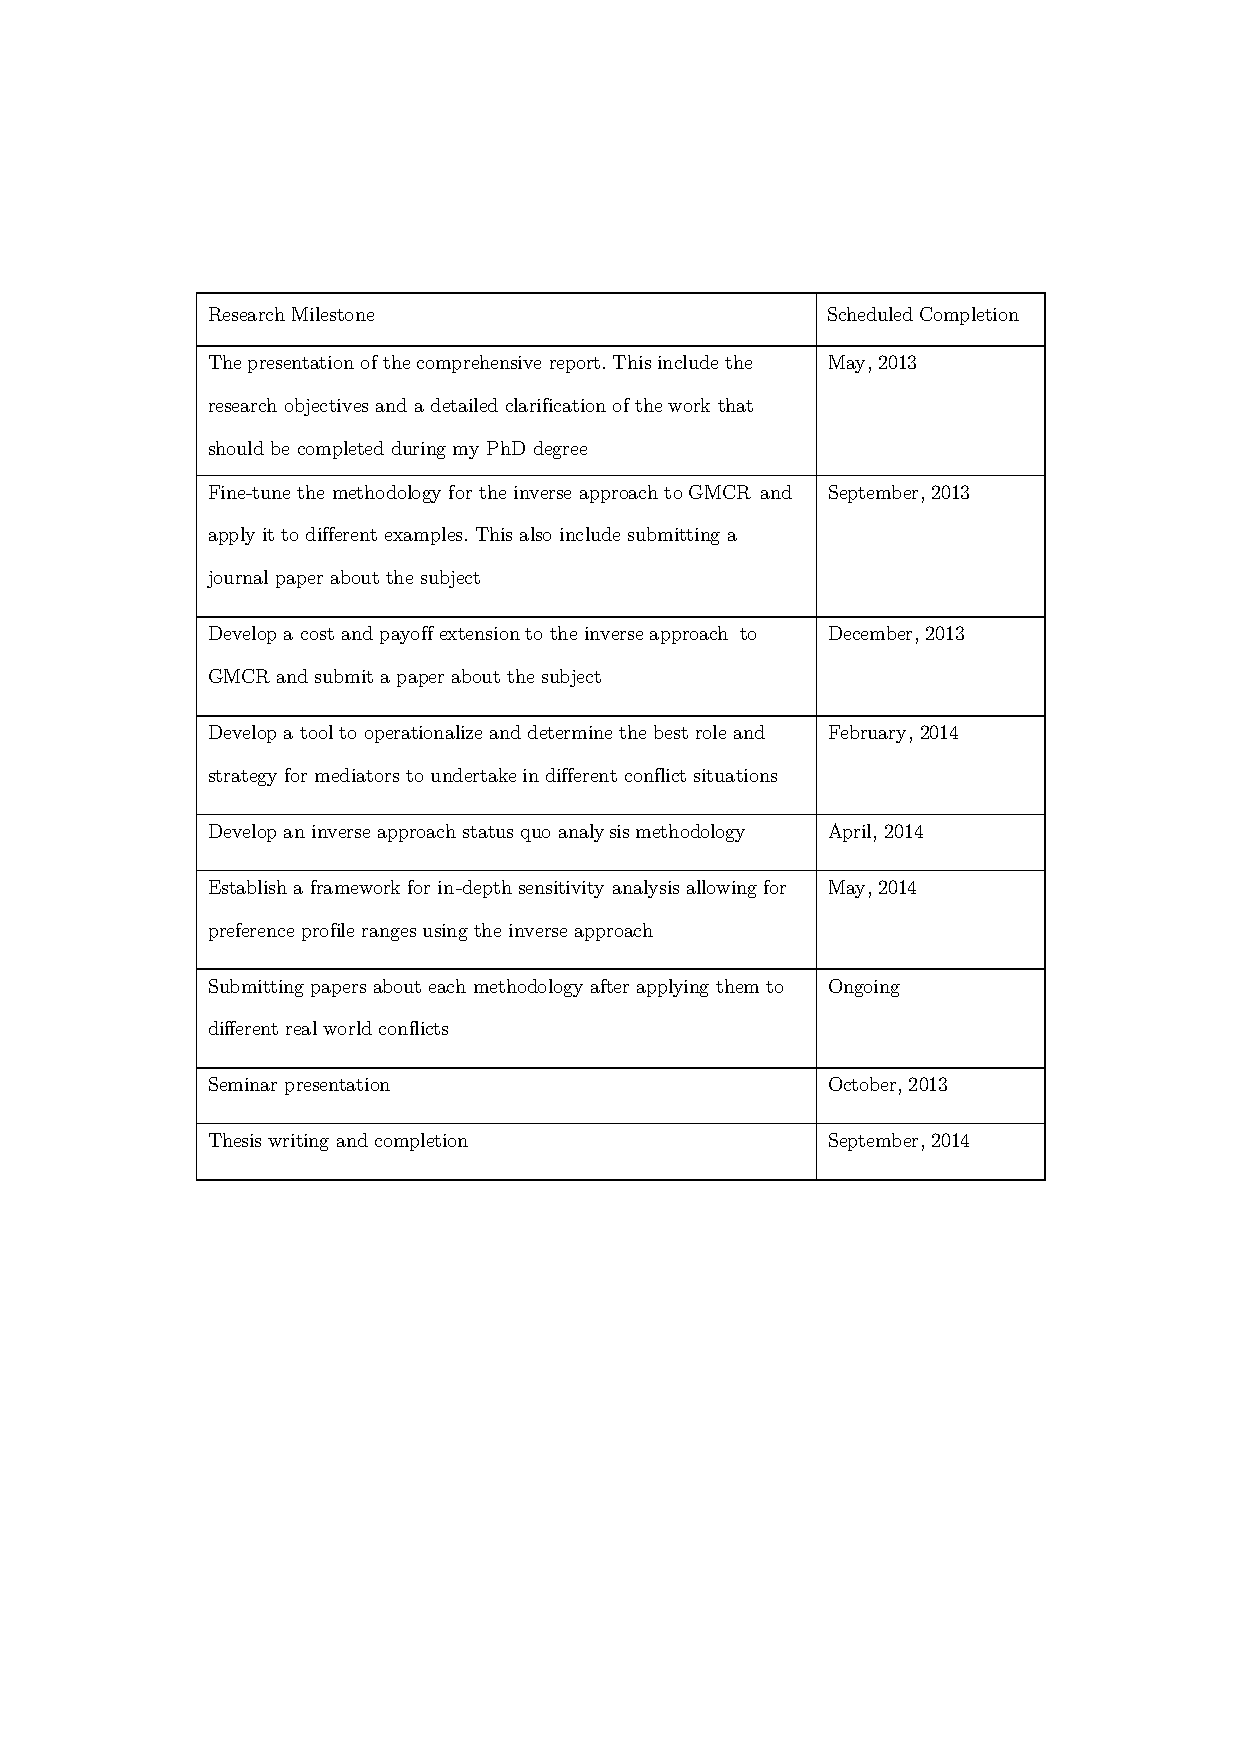
\includegraphics[scale=.8]{PDF-IMG/Research_Milestones.pdf}

\caption{Research Milestones and Schedule}

\label{tbl:milestones}
\end{table}
%======================================================================


%----------------------------------------------------------------------
% END MATERIAL
%----------------------------------------------------------------------

% B I B L I O G R A P H Y
% -----------------------

% The following statement selects the style to use for references.  It controls the sort order of the entries in the bibliography and also the formatting for the in-text labels.
\bibliographystyle{apalike}
% This specifies the location of the file containing the bibliographic information.  
% It assumes you're using BibTeX (if not, why not?).
\cleardoublepage % This is needed if the book class is used, to place the anchor in the correct page,
                 % because the bibliography will start on its own page.
                 % Use \clearpage instead if the document class uses the "oneside" argument
\phantomsection  % With hyperref package, enables hyperlinking from the table of contents to bibliography             
% The following statement causes the title "References" to be used for the bibliography section:
\renewcommand*{\bibname}{References}

% Add the References to the Table of Contents
\addcontentsline{toc}{chapter}{\textbf{References}}

\bibliography{uw-ethesisB}
% Tip 5: You can create multiple .bib files to organize your references. 
% Just list them all in the \bibliogaphy command, separated by commas (no spaces).

% The following statement causes the specified references to be added to the bibliography% even if they were not 
% cited in the text. The asterisk is a wildcard that causes all entries in the bibliographic database to be included (optional).

%\nocite{*}

\end{document}
